\documentclass[12pt]{ociamthesis}  % default square logo 
%\documentclass[12pt,beltcrest]{ociamthesis} % use old belt crest logo
%\documentclass[12pt,shieldcrest]{ociamthesis} % use older shield crest logo

%load any additional packages
\usepackage{amssymb}
\usepackage{listings}

\usepackage{color}
 
\definecolor{codegreen}{rgb}{0,0.6,0}
\definecolor{codegray}{rgb}{0.5,0.5,0.5}
\definecolor{codepurple}{rgb}{0.58,0,0.82}
\definecolor{backcolour}{rgb}{0.95,0.95,0.92}

 
\lstdefinestyle{mystyle}{
    backgroundcolor=\color{backcolour},   
    commentstyle=\color{codegreen},
    keywordstyle=\color{magenta},
    numberstyle=\tiny\color{codegray},
    stringstyle=\color{codepurple},
    basicstyle=\footnotesize,
    breakatwhitespace=false,         
    breaklines=true,                 
    captionpos=b,                    
    keepspaces=true,                 
    numbers=left,                    
    numbersep=5pt,                  
    showspaces=false,                
    showstringspaces=false,
    showtabs=false,                  
    tabsize=2,
    language=sh
}

\lstset{style=mystyle}

%input macros (i.e. write your own macros file called mymacros.tex 
%and uncomment the next line)
%\include{mymacros}

\title{Modul Praktikum \\[1ex]     %your thesis title,
        Kecerdasan Buatan}   %note \\[1ex] is a line break in the title

\author{Rolly Maulana Awangga}             %your name
\college{0410118609\\[5ex]
Applied Bachelor of Informatics Engineering}  %your college

%\renewcommand{\submittedtext}{change the default text here if needed}
\degree{Politeknik Pos Indonesia}     %the degree
\degreedate{Bandung 2019}         %the degree date

%end the preamble and start the document
\begin{document}

%this baselineskip gives sufficient line spacing for an examiner to easily
%markup the thesis with comments
\baselineskip=18pt plus1pt

%set the number of sectioning levels that get number and appear in the contents
\setcounter{secnumdepth}{3}
\setcounter{tocdepth}{3}


\maketitle                  % create a title page from the preamble info
\include{section/dedication}        % include a dedication.tex file
\include{section/acknowlegements}   % include an acknowledgements.tex file
\include{section/abstract}          % include the abstract

\begin{romanpages}          % start roman page numbering
\tableofcontents            % generate and include a table of contents
\listoffigures              % generate and include a list of figures
\end{romanpages}            % end roman page numbering

%now include the files of latex for each of the chapters etc
\chapter{Mengenal Kecerdasan Buatan dan Scikit-Learn}
Buku umum yang digunakan adalah \cite{russell2016artificial} dan  
untuk sebelum UTS menggunakan buku \textit{Python Artificial Intelligence Projects for Beginners}\cite{eckroth2018python}.
Dengan praktek menggunakan python 3 dan editor anaconda dan library python scikit-learn.
Tujuan pembelajaran pada pertemuan pertama antara lain:
\begin{enumerate}
\item
Mengerti definisi kecerdasan buatan, sejarah kecerdasan buatan, perkembangan dan penggunaan di perusahaan
\item
Memahami cara instalasi dan pemakaian sci-kit learn
\item
Memahami cara penggunaan variabel explorer di spyder
\end{enumerate}
Tugas dengan cara dikumpulkan dengan pull request ke github dengan menggunakan latex pada repo yang dibuat oleh asisten riset.

\section{Teori}
Praktek teori penunjang yang dikerjakan :
\begin{enumerate}
\item
Buat Resume Definisi, Sejarah dan perkembangan Kecerdasan Buatan, dengan bahasa yang mudah dipahami dan dimengerti. Buatan sendiri bebas plagiat[hari ke 1](10)
\item
Buat Resume mengenai definisi supervised learning, klasifikasi, regresi dan unsupervised learning. Data set, training set dan testing set.[hari ke 1](10)
\end{enumerate}

\section{Instalasi}
Membuka https://scikit-learn.org/stable/tutorial/basic/tutorial.html. Dengan menggunakan bahasa yang mudah dimengerti dan bebas plagiat. 
Dan wajib skrinsut dari komputer sendiri.
\begin{enumerate}
\item
Instalasi library scikit dari anaconda, mencoba kompilasi dan uji coba ambil contoh kode dan lihat variabel explorer[hari ke 1](10)
\item
Mencoba Loading an example dataset, menjelaskan maksud dari tulisan tersebut dan mengartikan per baris[hari ke 1](10)
\item
Mencoba Learning and predicting, menjelaskan maksud dari tulisan tersebut dan mengartikan per baris[hari ke 2](10)
\item
mencoba Model persistence, menjelaskan maksud dari tulisan tersebut dan mengartikan per baris[hari ke 2](10)
\item 
Mencoba Conventions, menjelaskan maksud dari tulisan tersebut dan mengartikan per baris[hari ke 2](10)
\end{enumerate}


\section{Penanganan Error}
Dari percobaan yang dilakukan di atas, apabila mendapatkan error maka:

\begin{enumerate}
	\item
	skrinsut error[hari ke 2](10)
	\item
Tuliskan kode eror dan jenis errornya [hari ke 2](10)
	\item
Solusi pemecahan masalah error tersebut[hari ke 2](10)

\end{enumerate}


\section{andi muh aslam/1164064}
\subsection{sejarah dan perkembangan kecerdasan buatan}
\begin{enumerate}
\item didefinisikan  kecerdasan yang ditunjukkan oleh suatu entitas buatan. Umumnya dianggap komputer. Kecerdasan Buatan (Artificial Intelligence atau AI) didefinisikan sebagai kecerdasan yang ditunjukan oleh suatu entitas buatan. Sistem seperti ini umumnnya dianggao kemputer. Kecerdasan dimasukkan ke dalam mesin (komputer) agar dapat melakukan pekerjaan seperti yang dapat dilakukan manusia. Kecerdasan Buatan (Artificial Intelligence atau AI) didefinikasikan sebagai kecerdasan yang ditinjukkan oleh suatu entitas buatan. Sistem seperti ini umumnya di anggap komputer. Kecerdasan diciptakan dan dimasukkan melakukan pekerjaan seperti yang dapat dilakukan manusia. 
\item Sejarah dan perkembangan kecerdasan buatan terjadi pada musim panas tahun 1956 tercatat adanya seminar mengenai AI di Darmouth College. Seminar pada waktu itu dihadiri oleh sejumlah pakar komputer dan membahas potensi komputer dalam meniru 
kepandaian manusia. Akan tetapi perkembangan yang sering terjadi semenjak diciptakannya LISP, yaitu bahasa kecerdasan buatan yang dibuat tahun 1960 oleh John McCarthy. Istilah pada kecerdasan buatan atau Artificial Intelligence diambil dari Marvin Minsky dari MIT. Dia menulis karya ilmiah berjudul Step towards Artificial Intelligence,The Institute of radio Engineers Proceedings 49, January 1961\cite{nasution2012implementasi}.
\item Supervised learning merupakan sebuah pendekatan dimana sudah terdapat data yang dilatih, dan terdapat variable yang ditargetkan sehingga tujuan dari pendekatan ini adalah mengkelompokan suatu data ke data yang sudah ada. Sedangkan unsupervised 
learning tidak memiliki data latih, sehingga dari data yang ada, kita mengelompokan data tersebut menjadi 2 bagian atau 3 bagian dan seterusnya.
\item Klasifikasi adalah salah satu topik utama dalam data mining atau machine learning. Klasifikasi yaitu suatu pengelompokan data dimana data yang digunakan tersebut mempunyai kelas label atau target.
\item Regresi adalah Supervised learning tidak hanya mempelajari classifier, tetapi juga mempelajari fungsi yang dapat memprediksi suatu nilai numerik. Contoh, ketika diberi foto seseorang, kita ingin memprediksi umur, tinggi, dan berat orang yang ada pada foto tersebut.
\item Data set adalah cabang aplikasi dari Artificial Intelligence/Kecerdasan Buatan yang fokus pada pengembangan sebuah sistem yang mampu belajar sendiri tanpa harus berulang kali di program oleh manusia.
\item Training set yaitu jika pasangan objek, dan kelas yang menunjuk pada objek tersebut adalah suatu contoh yang telah diberi label akan menghasilkan suatu algoritma pembelajaran.
\subitem Testing set digunakan untuk mengukur sejauh mana classifier berhasil melakukan klasifikasi dengan benar\cite{darujati2012pemanfaatan}.
\end{enumerate}


\section{Instalasi}
untuk instalasi mencakup i beberapa pembahasan dan tutorial. yaitu :
\begin{enumerate}
\item Instalasi Scikit-Learn dari Anaconda
\end{enumerate}

\begin{figure} [ht]
\centering
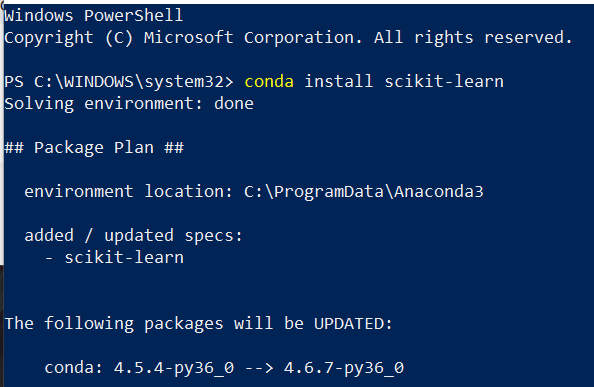
\includegraphics[scale=1] {figures/1.png}
\caption{masukkan perintah 'conda install scikit-learn' maka anaconda akan terinstall}
\label{proses instalasi}
\end{figure}


\begin{figure} [ht]
\centering
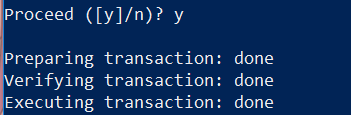
\includegraphics[scale=1] {figures/2.png}
\caption{Kemudian akan muncuk proceed ([y]/n)? di sini saya memilih perintah 'y' untuk menyetujui proceed tersebut}
\label{proses instalasi}
\end{figure}

\begin{figure} [ht]
\centering 
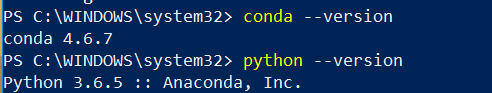
\includegraphics[scale=1] {figures/3.png}
\caption{conda --version dan python --version perintah untuk memunculkan versi dari anaconda dan python tersebut }
\label{proses instalasi}
\end{figure}

\begin{figure} [ht]
\centering 
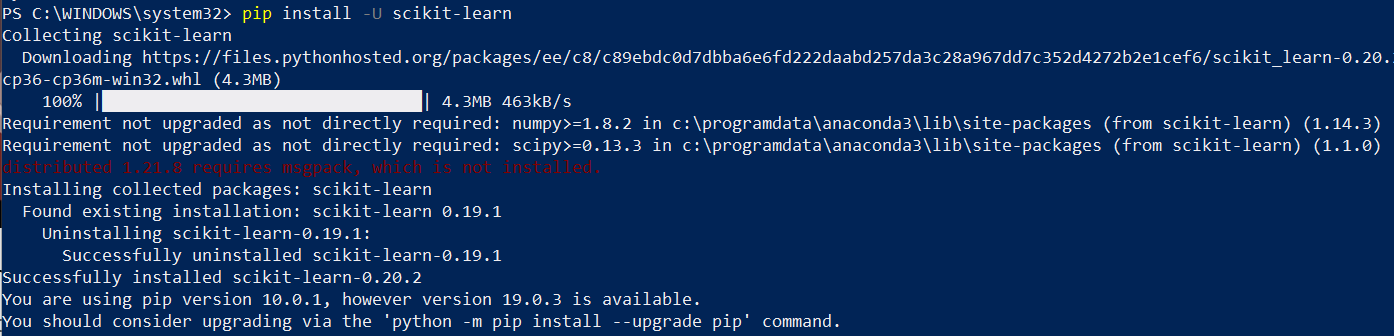
\includegraphics[scale=1] {figures/4.png}
\caption{perintah untuk install scikit-learn }
\label{proses instalasi}
\end{figure}

\begin{figure} [ht]
\centering 
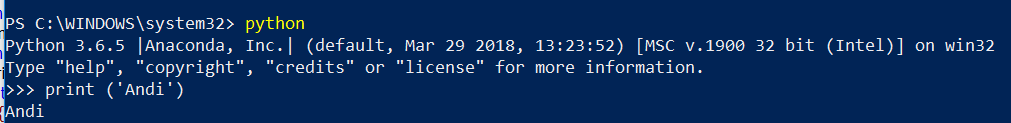
\includegraphics[scale=1] {figures/5.png}
\caption{perintah Print untuk memunculkan data yang ingin di tampilkan di sini saya menampilkan data ('Andi') }
\label{proses instalasi}
\end{figure}

\section{Aip Suprapto Munari/1164063}
\subsection{Teori}
\begin{enumerate}
\item Definisi, sejarah, dan perkembangan kecerdasan buatan.
\subitem Definisi kecerdasan buatan adalah ilmu pengetahuan yang dapat membuat komputer untuk meniru kecerdasan manusia yang berhubungan dengan penangkapan, pemodelan, dan penyimpanan kecerdasan manusia dalam sebuah sistem teknologi. Contohnya yaitu melakukan analisa penalaran untuk mengambil suatu kesimpulan atau penerjemahan atau keputusan dari satu bahasa satu ke bahasa lain.
\subitem Sejarah dan perkembangan kecerdasan buatan terjadi pada musim panas tahun 1956 tercatat adanya seminar mengenai AI di Darmouth College. Seminar pada waktu itu dihadiri oleh sejumlah pakar komputer dan membahas potensi komputer dalam meniru kepandaian manusia. Akan tetapi perkembangan yang sering terjadi semenjak diciptakannya LISP, yaitu bahasa kecerdasan buatan yang dibuat tahun 1960 oleh John McCarthy. Istilah pada kecerdasan buatan atau Artificial Intelligence diambil dari Marvin Minsky dari MIT. Dia menulis karya ilmiah berjudul Step towards Artificial Intelligence, The Institute of radio Engineers Proceedings 49, January 1961\cite{baraja2008kecerdasan}. 
\item  Definisi supervised learning, klasifikasi, regresi, dan unsupervised learning. Data set, training set dan testing set. 
\subitem Supervised learning merupakan sebuah pendekatan dimana sudah terdapat data yang dilatih, dan terdapat variable yang ditargetkan sehingga tujuan dari pendekatan ini adalah mengkelompokan suatu data ke data yang sudah ada. Sedangkan unsupervised learning tidak memiliki data latih, sehingga dari data yang ada, kita mengelompokan data tersebut menjadi 2 bagian atau 3 bagian dan seterusnya.
\subitem Klasifikasi merupakan salah satu topik utama dalam data mining atau machine learning. Klasifikasi yaitu suatu pengelompokan data dimana data tersebut digunakan untuk mempunyai kelas label atau target.
\subitem Regresi adalah Supervised learning tidak hanya mempelajari classifier, tetapi juga mempelajari fungsi yang dapat memprediksi suatu nilai numerik. Contoh, ketika diberi foto seseorang, kita ingin memprediksi umur, tinggi, dan berat orang yang ada pada foto tersebut.
\subitem Data set adalah cabang aplikasi dari Artificial Intelligence/Kecerdasan Buatan yang fokus pada pengembangan sebuah sistem yang mampu belajar sendiri tanpa harus berulang kali di program oleh manusia.
\subitem Training set yaitu jika pasangan objek, dan kelas yang menunjuk pada objek tersebut adalah suatu contoh yang telah diberi label akan menghasilkan suatu algoritma pembelajaran.
\subitem Testing set digunakan untuk mengukur sejauh mana classifier berhasil melakukan klasifikasi dengan benar\cite{zhu2009introduction}.
\end{enumerate}
\subsection{Instalasi}
\subsubsection{Instalasi Library Scikit dari Anaconda}
\begin{enumerate}
\item Download aplikasi Anaconda terlebih dahulu. Lihat pada gambar 1.1
\item Install aplikasi Anaconda yang sudah di download tadi. Lihat pada gambar 1.2
\item Centang Keduanya lalu tekan tombol install. Lihat pada gambar 1.3
\item Setelah itu tunggu sampai proses instalasi selesai lalu jika sudah tekan tombol finish. Lihat pada gambar 1.4
\item Lalu buka command prompt anda dan tuliskan perintah berikut ini untuk mengecek apakah aplikasinya sudah terinstall. Lihat pada gambar 1.5
\item Kemudian ketikkan perinta pip install -U scikit-learn seperti gambar berikut. Lihat pada gambar 1.6
\item Lalu jika sudah  ketikkan juga perintah conda install scikit-learn. Lihat pada gambar 1.7
\item dan setelah itu pilih y. Lihat pada gambar 1.8
\item Hasil version yang diinstall. Lihat pada gambar 1.9
\end{enumerate}
\subsubsection{Mencoba Loading an example Dataset}
\begin{itemize}
\item from sklearn import datasets(pada baris ini merupakan sebuah perintah untuk mengimport class datasets dari packaged sklearn).
\item iris = datasets.load\_iris()(pada baris kedua ini dimana iris merupakan suatu estimator/parameter yang berfungsi untuk mengambil data pada item datasets.load\_iris).
\item digits = datasets.load\_digits()(pada baris ketiga ini dimana digits merupakan suatu estimator/parameter yang berfungsi untuk mengambil data pada item datasets.load\_digits).
\item print(digits.data)(pada baris keempat ini merupakan perintah yang berfungsi untuk menampilkan estimator/parameter yang dipanggil pada item digits.data dan menampilkan outputannya) Lihat gambar 1.10.
\item digits.target(barisan ini untuk mengambil target pada estimator/parameter digits dan menampilkan outputannya) Lihat gambar 1.11.
\item digits.images[0](barisan ini untuk mengambil images[0] pada estimator/parameter digits dan menampilkan outputannyal) Lihat gambar 1.12.
\end{itemize}
\subsubsection{Learning and Predicting}
\begin{itemize}
\item from sklearn import svm(pada baris ini merupakan sebuah perintah untuk mengimport class svm dari packaged sklearn).
\item clf = svm.SVC(gamma=0.001, C=100.)(pada baris kedua ini clf sebagai estimator/parameter, svm.SVC sebagai class, gamma sebagai parameter untuk menetapkan nilai secara manual)
\item clf.fit(digits.data[:-1], digits.target[:-1])(pada baris ketiga ini clf sebagai estimator/parameter, fit sebagai metode, digits.data sebagai item, [:-1] sebagai syntax pythonnya dan menampilkan outputannya) Lihat gambar 1.13.
\item clf.predict(digits.data[-1:])
\end{itemize}
\subsection{Mencoba Model Persistance, menjelaskan maksud dari tulisan tersebut dan mengartikan per baris}
\begin{enumerate}
\item
Pada Python Shell ketikan "from sklearn import svm" artinya akan mengimport sebuah Support Vector Machine(SVM) yang merupakan algoritma classification yang akan diambil dari Scikit-Learn.
\item
Kemudian, lanjutkan dengan "from sklearn import datasets" yang artinya akan mengambil package datasets dari Scikit-Learn.
\item
ketikan, clf = svm.SVC(gamma='scale') berfungsi untuk mendeklarasikan suatu value yang bernama clf yang berisi gamma. Parameter gamma menentukan seberapa jauh pengaruh dari satu contoh training.
\item
Ketikan, X, y = iris.data, iris.target, artinya X sebagai data iris, dan y merupakan larik target.
\item
Ketikan, clf.fit(X, y) berfungsi untuk melakukan pengujian classifier. hasilnya seperti ini
\begin{figure}
	\begin{center}
   	 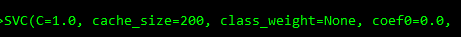
\includegraphics[scale=1]{figures/aip7.png}
   	 \caption{Hasil Pengujian Classifier}	
	\end{center}
\end{figure}
\item
\begin{figure}
	\begin{center}
   	 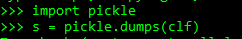
\includegraphics[scale=1]{figures/aip8.png}
   	 \caption{Hasil Pengujian Classifier}	
	\end{center}
\end{figure}
Dari gambar diatas dapat dijelaskan bahwa akan mengimport Pickle dari Python. Pickle digunakan untuk serialisasi dan de-serialisasi struktur objek Python. Objek apa pun dengan Python dapat di-Pickle sehingga dapat disimpan di disk. kemudian menyimpan data objek ke file CLF sebelumnya dengan menggunakan function pickle.dumps(clf).
\item
Setelah mengetikan fungsi fungsi diatas, selanjutnya ketikan "clf2 = pickle.loads(s)" yang artinya pickle.loads digunakan untuk memuat data pickle dari string byte. "S" dalam loads mengacu pada fakta bahwa dalam Python 2, data dimuat dari string.
\begin{figure}
	\begin{center}
   	 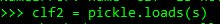
\includegraphics[scale=1]{figures/aip9.png}
   	 \caption{Pickle Pada Python}	
	\end{center}
\end{figure}
\item
\begin{figure}
	\begin{center}
   	 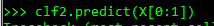
\includegraphics[scale=1]{figures/aip10.png}
   	 \caption{Pengujian Classifier Pickle}	
	\end{center}
\end{figure}
Pada gambar diatas dilakukan pengujian nilai baru dengan menggunakan "cf2.predict(X[0:1])" dengan target asumsinya (0,1) hasilnya berbentuk array.
\item
Dalam kasus khusus scikit-learn, mungkin lebih menarik untuk menggunakan joblib (dump dan load) untuk menggantikan Pickle, yang lebih efisien pada data besar tetapi hanya bisa di Pickle ke disk dan tidak ke string. untuk menggunakan Joblib pertama ketikan "from joblib import dump , load" yang artinya akan Merekonstruksi objek Python dari file yang sudah ada.\\

dump(clf, 'filename.joblib') akan merekontruksi file CLF yang tadi sudah dideklarasikan.\\
clf = load('filename.joblib') untuk mereload model yang sudah di Pickle\\
\begin{figure}
	\begin{center}
   	 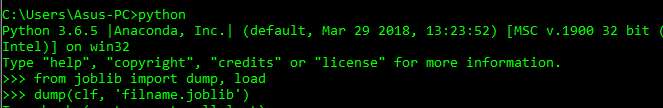
\includegraphics[scale=1]{figures/aip11.png}
   	 \caption{Penggunaan Joblib}	
	\end{center}
\end{figure}
\end{enumerate}

\subsection{Mencoba Conventions, menjelaskan maksud dari tulisan tersebut dan mengartikan per baris}
\begin{enumerate}
\item
Import numpy as np, digunakan untuk mengimport Numpy sebagai np.\\
From sklearn import randomprojection artinya modul yang mengimplementasikan cara sederhana dan efisien secara komputasi untuk mengurangi dimensi data dengan memperdagangkan sejumlah akurasi yang terkendali (sebagai varian tambahan) untuk waktu pemrosesan yang lebih cepat dan ukuran model yang lebih kecil.
\begin{figure}
	\begin{center}
   	 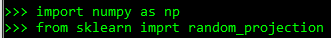
\includegraphics[scale=1]{figures/aip12.png}
   	 \caption{Deklarasi Numpy}	
	\end{center}
\end{figure}
\item
\begin{figure}
	\begin{center}
   	 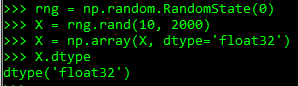
\includegraphics[scale=1]{figures/aip13.png}
   	 \caption{Contoh Type Casting}	
	\end{center}
\end{figure}
Pada gambar diatas dapat dijelaskan bahwa :\\
rng = np.random.RandomState(0), digunakan untuk menginisialisasikan random number generator.\\
X = rng.rand(10, 2000) artinya akan merandom value antara 10 sampai 2000.\\
X = np.array(X, dtype='float32') Array numpy terdiri dari buffer memori "mentah" yang diartikan sebagai array melalui "views". Anda dapat menganggap semua array numpy sebagai tampilan. Mendeklarasikan X sebagai float32.
\item
Dalam contoh ini, X adalah float32, yang dilemparkan ke float64 oleh fittransform (X).
\begin{figure}
	\begin{center}
   	 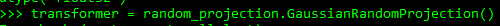
\includegraphics[scale=1]{figures/aip14.png}
   	 \caption{Menggunakan FitTransform}
	\end{center}
\end{figure}
\item
Target regresi dilemparkan ke float64 dan target klasifikasi dipertahankan.

list(clf.predict(irisdata[:3])), akan memprediksi 3 data dari iris.\\
clf.fit irisdata, iristargetnames[iristarget] menguji classifier dengan ada targetnya yaitu irisnya sendiri.\\
list(clf.predict(irisdata[:3])), setelah diuji maka akan muncul datanya seperti dibawah ini\\
\begin{figure}
	\begin{center}
   	 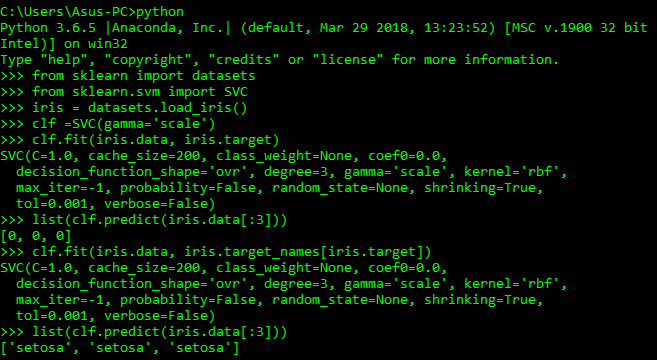
\includegraphics[scale=1]{figures/aip15.png}
   	 \caption{Regresi Yang Dilempar}
	\end{center}
\end{figure}
Di sini, prediksi pertama () mengembalikan array integer, karena iristarget (array integer)yang digunakan sesuai. Prediksi kedua () mengembalikan array string, karena iristargetnames cocok.
\item
Refitting dan Memperbaharui Parameter

y = rngbinomial(1, 0.5, 100) , random value dengan angka binomial atau suku dua untuk y \\
clfsetparams(kernel='linear')fit(X, y) mengubahn kernel default menjadi linear \\
clfsetparams(kernel='rbf', gamma='scale')fit(X, y)  Di sini, kernel default rbf pertama kali diubah menjadi linear melalui\\ SVCsetparams () setelah estimator dibuat, dan diubah kembali ke rbf untuk mereparasi estimator dan membuat prediksi kedua.
\begin{figure}
	\begin{center}
   	 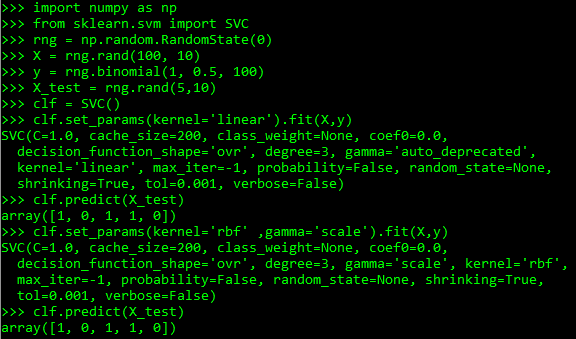
\includegraphics[scale=1]{figures/aip16.png}
   	 \caption{Refitting dan Memperbaharui Parameter}
	\end{center}
\end{figure}
\item
MultiClass VS MultiLabel Classifier \\
from sklearn.multiclass import OneVsRestClassifier ,adalah  ketika kita ingin melakukan klasifikasi multiclass atau multilabel dan baik unutk menggunakan OneVsRestClassifier per kelas. Untuk setiap classifier, kelas tersebut dipasang terhadap semua kelas lainnya. (Ini cukup jelas dan itu berarti bahwa masalah klasifikasi multiclass / multilabel dipecah menjadi beberapa masalah klasifikasi biner).\\
from sklearn.preprocessing import LabelBinarizer ,adalah kelas utilitas untuk membantu membuat matriks indikator label dari daftar label multi-kelas\\
Dalam gambar dibawah, classifier cocok pada array 1d label multiclass dan oleh karena itu metode predict () memberikan prediksi multiclass yang sesuai.
\begin{figure}
	\begin{center}
   	 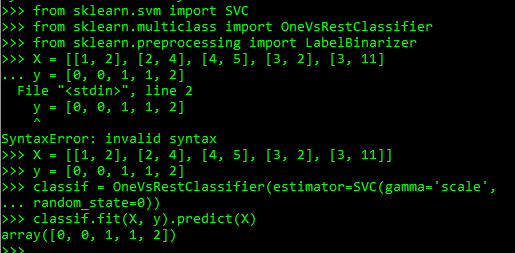
\includegraphics[scale=1]{figures/aip17.png}
   	 \caption{MultiClass Classifier}
	\end{center}
\end{figure}
\item
Di sini, classifier cocok () pada representasi label biner 2d dari y, menggunakan LabelBinarizer. Dalam hal ini predict () mengembalikan array 2d yang mewakili prediksi multilabel yang sesuai.
\begin{figure}
	\begin{center}
   	 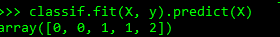
\includegraphics[scale=1]{figures/aip18.png}
   	 \caption{MultiClass Classifier biner 2D}
	\end{center}
\end{figure}
\item
from sklearn.preprocessing import MultiLabelBinarizer , artinya Transformasi antara iterable dari iterables dan format multilabel.\\
Dalam hal ini, penggolongnya sesuai pada setiap instance yang diberi beberapa label. MultiLabelBinarizer digunakan untuk membuat binarize array 2d dari multilabel agar sesuai. Hasilnya, predict () mengembalikan array 2d dengan beberapa label yang diprediksi untuk setiap instance.
\begin{figure}
	\begin{center}
   	 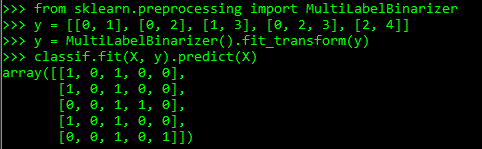
\includegraphics[scale=1]{figures/aip19.png}
   	 \caption{MultiLabel Classifier}
	\end{center}
\end{figure}
\end{enumerate}


\section{Penanganan Error}
HARI KEDUA
\begin{enumerate}
	\item
	Berikut ini merupakan eror yang ditemui pada saat melakukan percobaan skrip.
\begin{figure}
	\begin{center}
   	 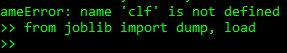
\includegraphics[scale=1]{figures/eror2.png}
   	 \caption{Eror Import}
	\end{center}
\end{figure}
	\item
Pada gambar eror diatas, kode erornya adalah "ImportError: No Module Named" artinya mengalami masalah saat mengimpor modul yang ditentukan.
	\item
Solusinya bisa dilakukan seperti berikut :\\
eror diats terjadi dikarenakan Library Joblib belum terinstal pada PC. Maka dari itu sekarang kita harus menginstalnya dulu.
	\item
Buka CMD, kemudian ketikan "pip install joblib" tunggu sampai instalasi berhasil seperti gambar berikut.
\begin{figure}
	\begin{center}
   	 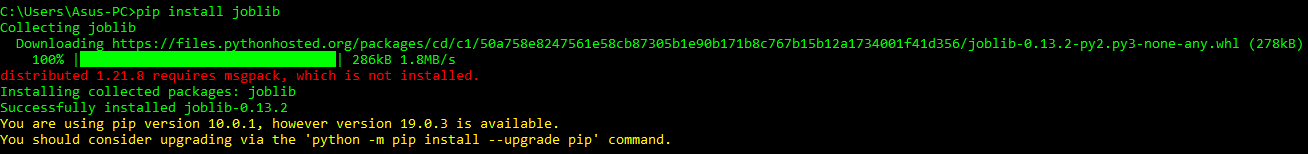
\includegraphics[scale=1]{figures/solusi2.png}
   	 \caption{Instal Library Joblib}
	\end{center}
\end{figure}
	\item
Apabila sudah terinstall, dapat dilakukan lagi import library joblib, maka akan berhasil seperti dibawah berikut
\begin{figure}
	\begin{center}
   	 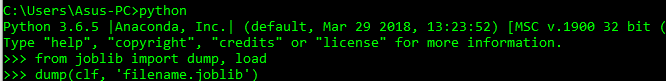
\includegraphics[scale=1]{figures/solusi2_1.png}
   	 \caption{Berhasil Import Library Joblib}
	\end{center}
\end{figure}
\end{enumerate}

\begin{figure}[ht]\centerline{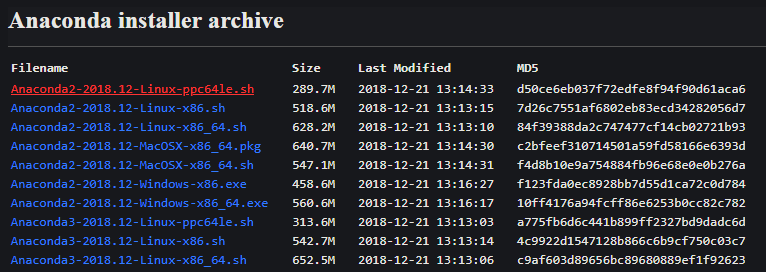
\includegraphics[width=1\textwidth]{figures/a1.PNG}}\caption{Download Anaconda.}\end{figure}
\begin{figure}[ht]\centerline{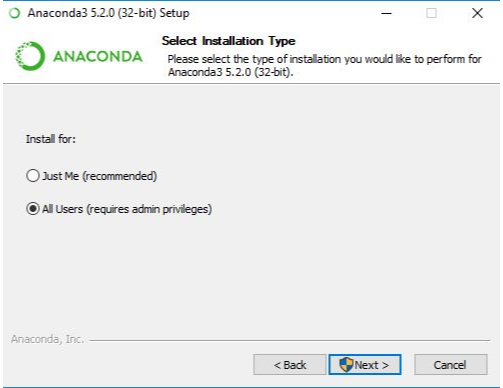
\includegraphics[width=0.75\textwidth]{figures/a2.PNG}}\caption{Langkah pertama instalasi anaconda.}\end{figure}
\begin{figure}[ht]\centerline{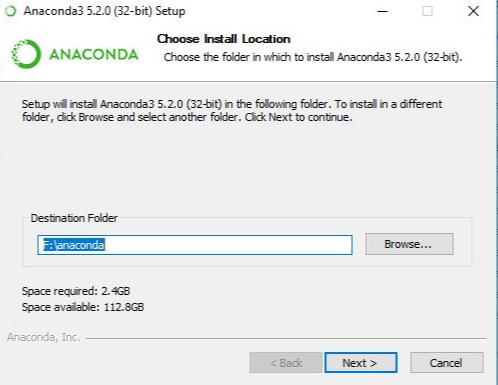
\includegraphics[width=0.75\textwidth]{figures/a3.PNG}}\caption{Langkah kedua instalasi anaconda.}\end{figure}
\begin{figure}[ht]\centerline{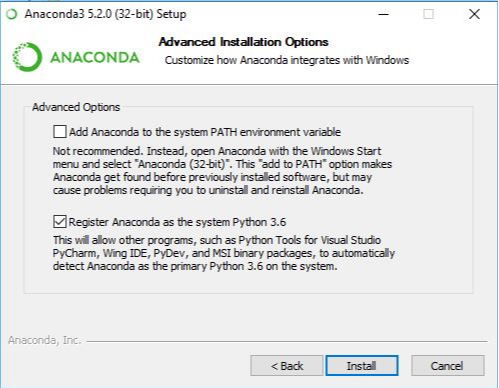
\includegraphics[width=0.75\textwidth]{figures/a4.PNG}}\caption{Langkah ketiga instalasi anaconda.}\end{figure}
\begin{figure}[ht]\centerline{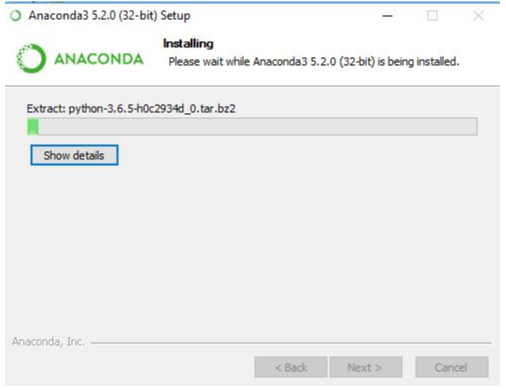
\includegraphics[width=0.75\textwidth]{figures/a5.PNG}}\caption{Langkah terakhir instalasi anaconda.}\end{figure}
\begin{figure}[ht]\centerline{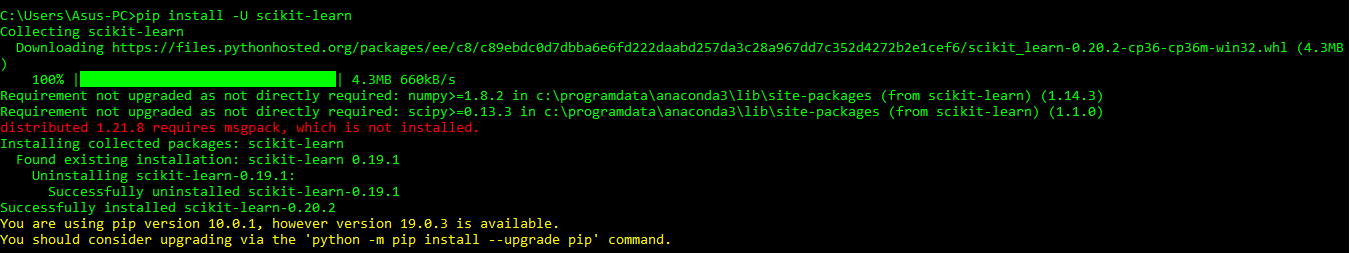
\includegraphics[width=0.75\textwidth]{figures/a6.PNG}}\caption{Langkah pertama instalasi scikit pada CMD.}\end{figure}
\begin{figure}[ht]\centerline{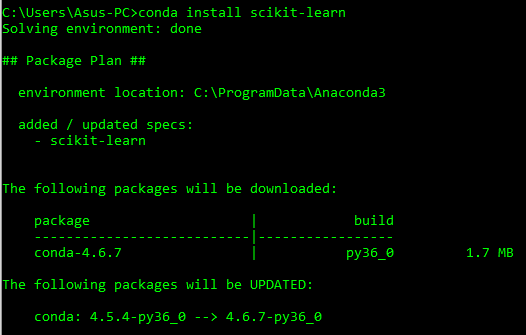
\includegraphics[width=0.75\textwidth]{figures/a7.PNG}}\caption{Langkah ketiga instalasi conda scikit pada CMD.}\end{figure}
\begin{figure}[ht]\centerline{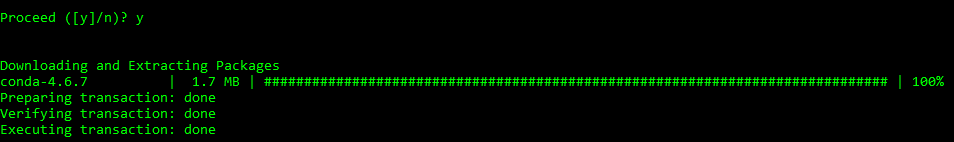
\includegraphics[width=0.75\textwidth]{figures/a8.PNG}}\caption{Langkah kedua pilih y.}\end{figure}
\begin{figure}[ht]\centerline{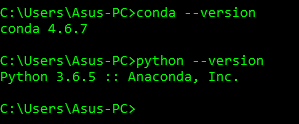
\includegraphics[width=0.75\textwidth]{figures/a9.PNG}}\caption{Langkah cek version yang diinstall.}\end{figure}
\begin{figure}[ht]\centerline{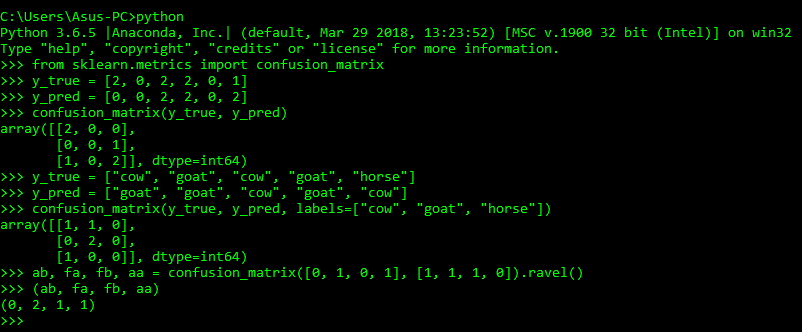
\includegraphics[width=0.75\textwidth]{figures/a10.PNG}}\caption{Hasil Tampilan 1.}\end{figure}
\begin{figure}[ht]\centerline{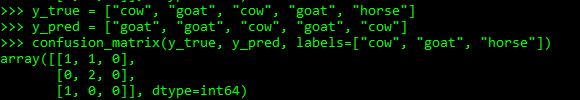
\includegraphics[width=0.75\textwidth]{figures/a11.PNG}}\caption{Hasil Tampilan 2.}\end{figure}
\begin{figure}[ht]\centerline{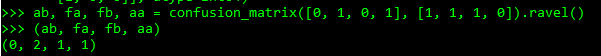
\includegraphics[width=0.75\textwidth]{figures/a12.PNG}}\caption{Hasil Tampilan 3.}\end{figure}




\chapter{Related Works}

Your related works, and your purpose and contribution which must be different as below.

\section{Aip Suprapto Munari/1164063}
\subsection{Teori}
\subsection{Binary Classification}
\begin{enumerate}
\item Binary Classification atau diartikan kedalam bahasa indonesia yaitu Klasifikasi Biner adalah tugas dalam mengkalrifikasikan elemen-elemen dari himpunan yang diberikan kedalam dua kelompok berdasarkan aturan klarifikasi. Pada ummnya klarifikasi biner akan jatuh ke dalam domain Supervised Learning dan dimana kasus khusus hanya memiliki dua kelas. Beberapa contoh yang meliputi Binary Classification adalah \begin{itemize}
		\item Deteksi Transaksi Penipuan Kartu Kredit
		\item Diagnosa medis
		\item Deteksi Spam
	\end{itemize}
\subitem Untuk contoh Binary Classification dapat dilihat pada gambar \ref{1}
		\begin{figure}[ht]
		\centerline{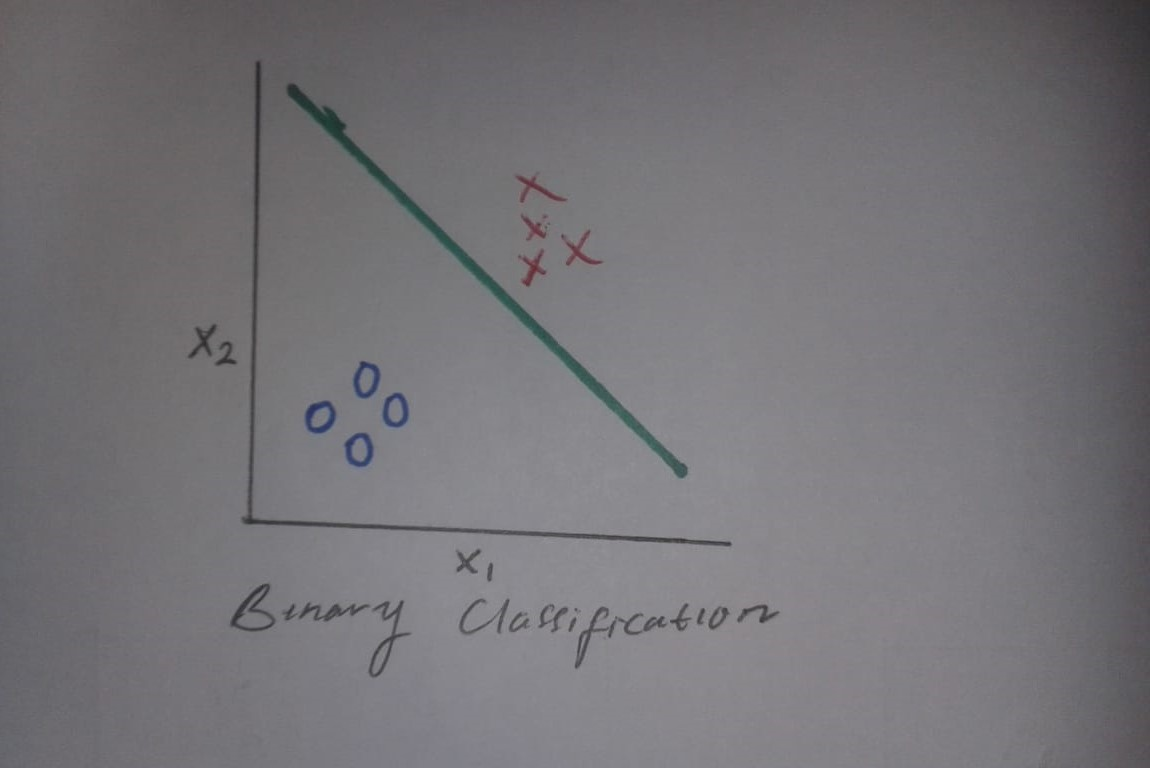
\includegraphics[width=1\textwidth]{figures/AIP/1.JPEG}}
		\caption{Binary Classification.}
		\label{1}
		\end{figure}
 \end{enumerate}

\subsection{Supervised Learning, Unsupervised Learning, Dan Classtering}
\begin{enumerate}
\item Supervised Learning merupakan sebuah pendekatan yang dimana sudah adanya sdata yang dilatih dan telah terdapat variabel yang telah ditargetkan sehingga bertujuan untuk mengelompokkan suatu data ke data yang sudah ada. Contoh dalam Supervised Learning yaitu ketika anda memiliki sejumlah buku yang yang telah dilabel dengan urutan kategori tertentu. Ketika anda akan membeli sebuah buku baru, maka harus di identifikasi isi dari buku tersebut dan memasukkannya kedalam kategori tertentu. Ketika anda membeli sebuah buku tersebut maka anda telah menerapkan sebuah logika fuzzy. Ilustrasi Supervised Learning dapat dilihat pada gambar \ref{2}.

		\begin{figure}[ht]
		\centerline{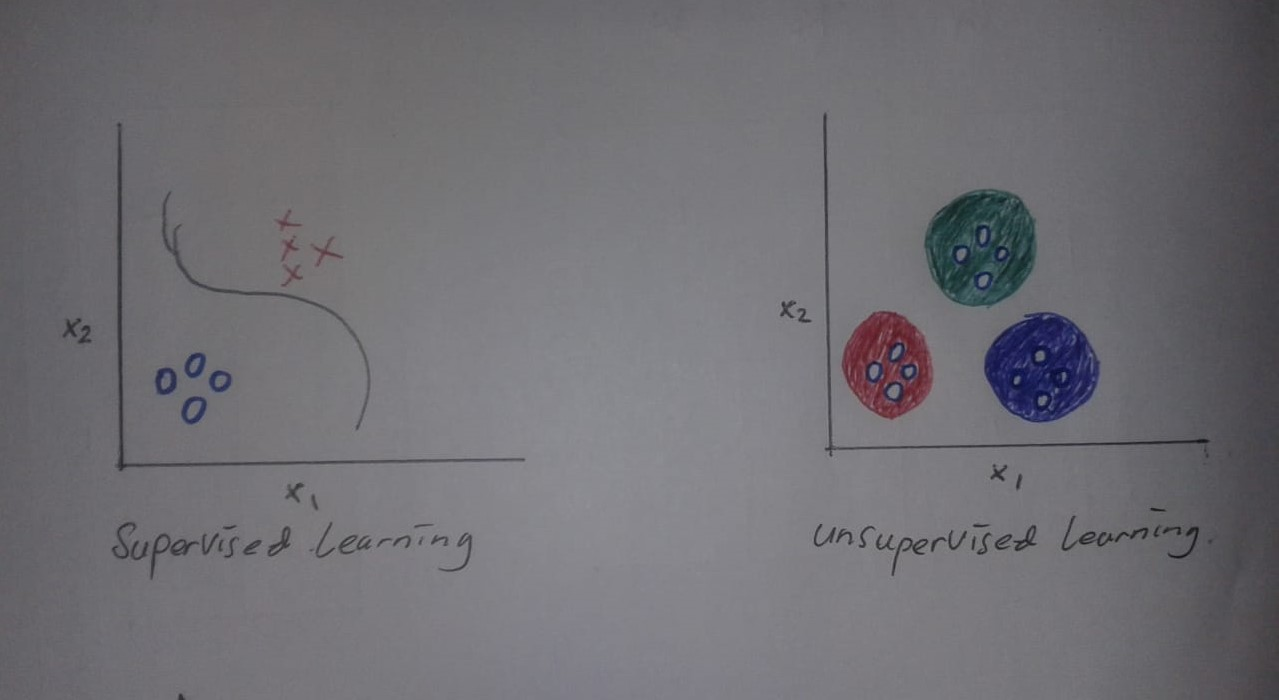
\includegraphics[width=1\textwidth]{figures/AIP/2.JPEG}}
		\caption{Supervised Learning.}
		\label{2}
		\end{figure}

\item Unsupervised Learning merupakan sebuah data yang belum ditentukan variabelnya jadi hanya berupa data saja. Dalam sebuah kasus Unsupervised Learning adalah aggap saja anda belum pernah membeli buku sama sekali dan pada suatu hari anda telah membeli buku dengan sangat banyak dalam kategori yang berbeda. Sehingga buku tersebut belum di kategorikan dan hanya berupa data buku saja. Ilustrasi Unsupervised Learning dapat dilihat pada gambar \ref{2}.

		\begin{figure}[ht]
		\centerline{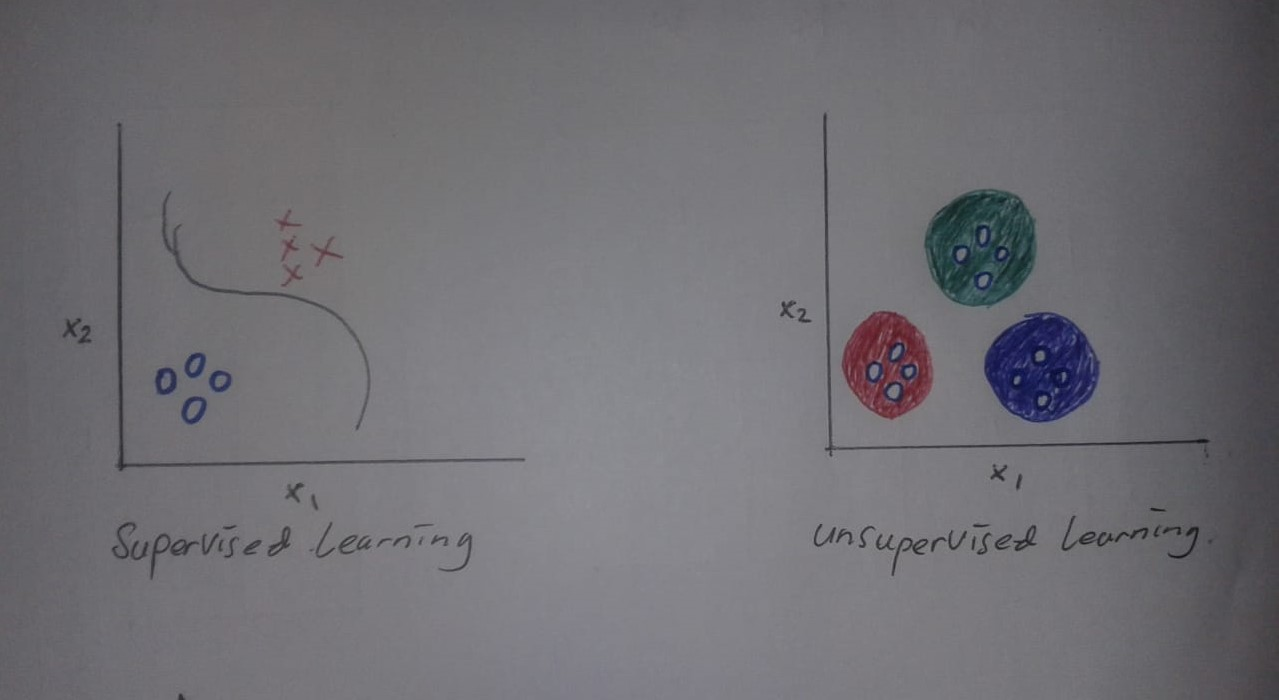
\includegraphics[width=1\textwidth]{figures/AIP/2.JPEG}}
		\caption{Unsupervised Learning.}
		\label{2}
		\end{figure}

\item Classtering merupakan sebuah proses untuk mengklasifikasikan sebuah data dalam satu parameter. Dalam kasus ini dapat dijelaskan ada beberapa orang yang memiliki kekuatan tubuh yang sehat dan kekuatan tubuh yang lemah. Parameter bagi orang yang memiliki tubuh yang kuat adalah orang yang terlihat bugar dan sehat maka dengan orang yang memiliki parameter adalah orang yang memiliki kekuatan tubuh yang kuat dan untuk kekuatan tubuh yang lemah adalah sebaliknya. Ilustrasi gambar dapat di lihat di gambar \ref{3}

		\begin{figure}[ht]
		\centerline{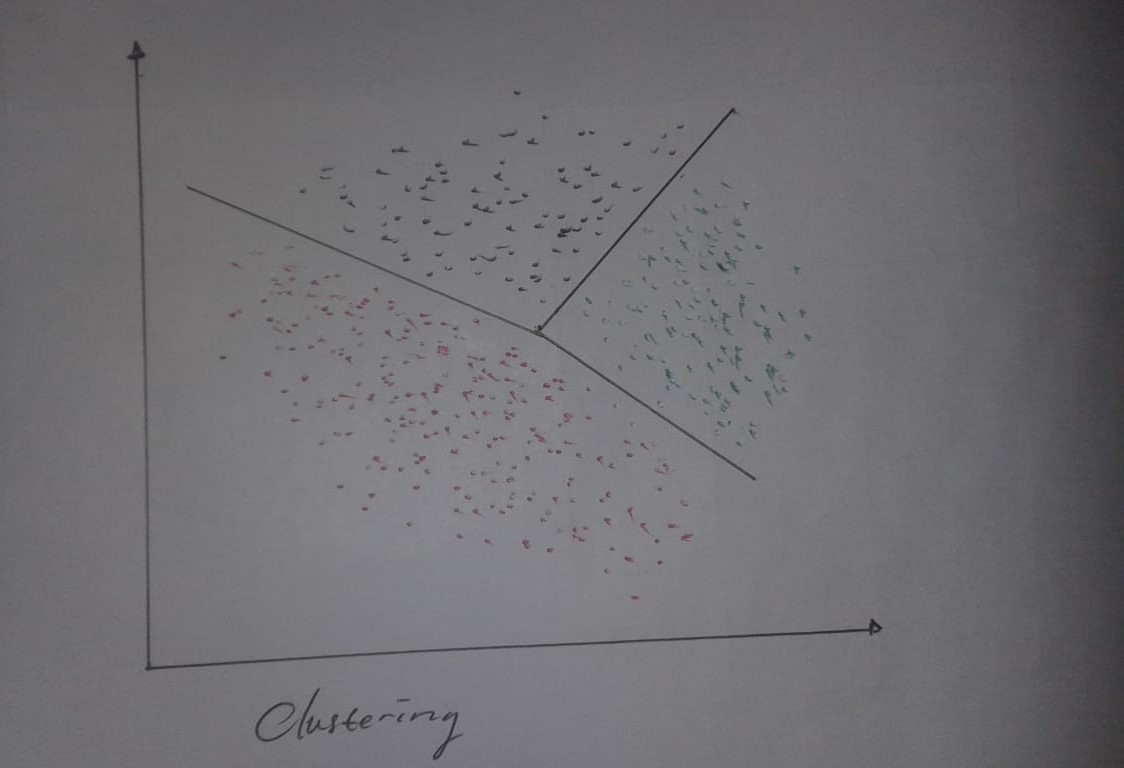
\includegraphics[width=1\textwidth]{figures/AIP/3.JPEG}}
		\caption{Clusterring.}
		\label{3}
		\end{figure}
\end{enumerate}

\subsection{Evaluasi Dan Akurasi}
\begin{enumerate}
\item Evaluasi dan akurasi adalah bagaimana cara kita dapat mengevaluasi sebarapa baik model melakukan pekerjaannya dengan cara mengukur akurasinya. Akurasi akan didefinisikan sebagai presentase kasus yang telah diklasifikasikan dengan benar. Kita dapat melakukan analisis kesalahan yang telah di buat oleh model.Dalam tabel tersebut baris true mangga dan true anggur menunjukkan kasus apakah itu objek mangga atau anggur. Kolom telah di prediksi dan dibuat oleh model. Ada 20 cow yang di prediksi benar dan ada 5 buffalo yang di prediksi salah. Ilustrasi dapat di lihat pada gambar \ref{4}

		\begin{figure}[ht]
		\centerline{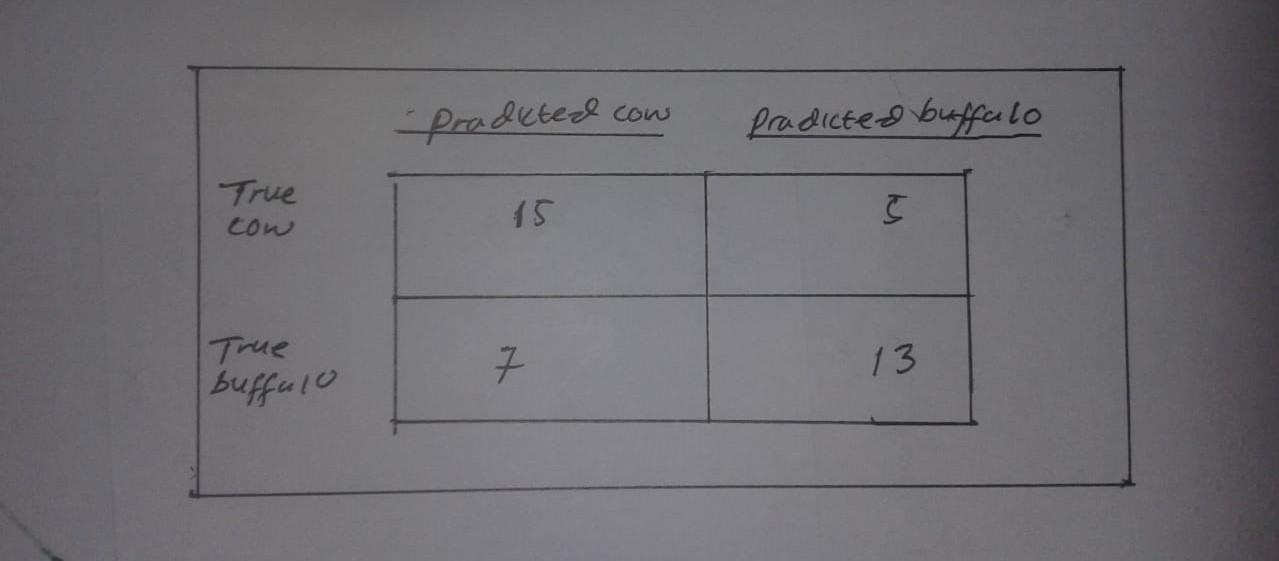
\includegraphics[width=1\textwidth]{figures/AIP/4.JPEG}}
		\caption{Evaluasi Dan Akurasi.}
		\label{4}
		\end{figure}
\end{enumerate}

\subsection{Confusion Matrix}
\begin{enumerate}
\item Ada beberapa cara untuk membuat dan membaca confusion matrix antara lain
	\begin{itemize}
		\item Tentukan pokok permasalahan serta atributnya
		\item Buat Decision Tree
		\item Buat Data Testing
		\item Mencari nilai variabelnya misal a,b,c, dan d
		\item Mencari nilai recall, precision, accuracy, dan erorr rate
	\end{itemize}
\subitem Di bawah ini adalah contoh dari confusion matrix
	\begin{verbatim}
		Recall =3/(1+3) = 0,75
		Precision = 3/(1+3) = 0,75
		Accuracy =(5+3)/(5+1+1+3) = 0,8
		Error Rate =(1+1)/(5+1+1+3) = 0,2 
	\end{verbatim}
\end{enumerate}

\subsection{Cara Kerja K-Fold Cross Validation}
\begin{enumerate}
\item Untuk cara kerja K-Fold Cross Validation adalah sebagai berikut
	\begin{itemize}
		\item Total instance dibagi menjadi N bagian.
		\item Fold yang pertama adalah bagian pertama menjadii testing data dan sisanya menjadi training data.
		\item Hitung akurasi berdasarkan porsi data tersebut dengan menggunakan persamaan.
		\item Fold yang ke dua adalah bagian ke dua menjadi testing data dan sisanya training data. 
		\item Hitung akurasi berdasarkan porsi data tersebut.
		\item Lakukan step secara berulang hingga habis mencapai fold ke-K.
		\item Terakhir hitung rata-rata akurasi K buah.
	\end{itemize}

\subitem Untuk ilustrasi K-Fold Cross Validation data di lihat pada gambar \ref{5}
		\begin{figure}[ht]
		\centerline{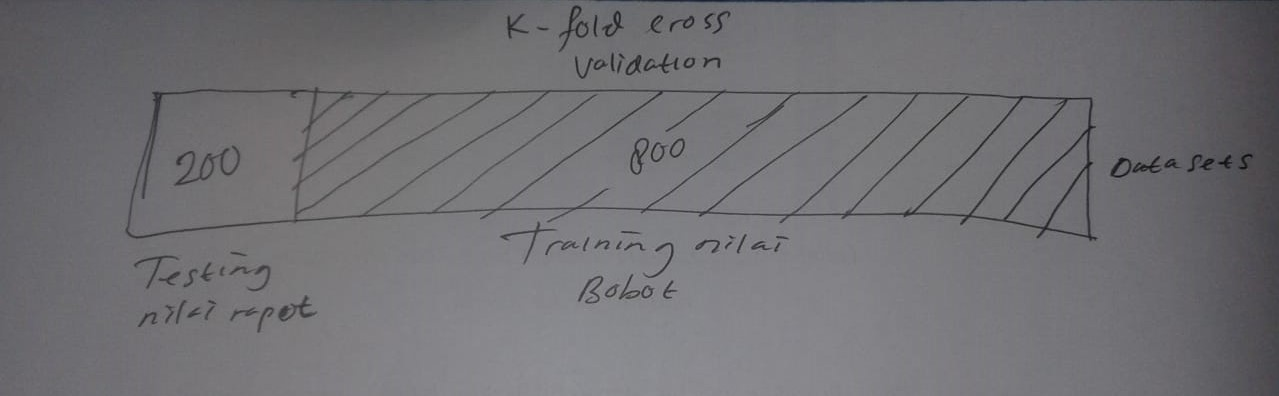
\includegraphics[width=1\textwidth]{figures/AIP/5.JPEG}}
		\caption{K-Fold Cross Validation.}
		\label{5}
		\end{figure}
\end{enumerate}

\subsection{Decision Tree}
\begin{enumerate}
\item Decision Tree adalah sebuah metode pembelajaran yang digunakan untuk melakukan klarifikasi dan regresi. Decision Tree digunakan untuk membuat sebuah model yang dapat memprediksi sebuah nilai variabel target dengan cara mempelajari aturan keputusan dari fitur data. Contoh Decision Tree adalah untuk melakukan predikisi apakah Sapi termasuk hewan herbivora atau bukan, lihat pada gambar \ref{6}.

		\begin{figure}[ht]
		\centerline{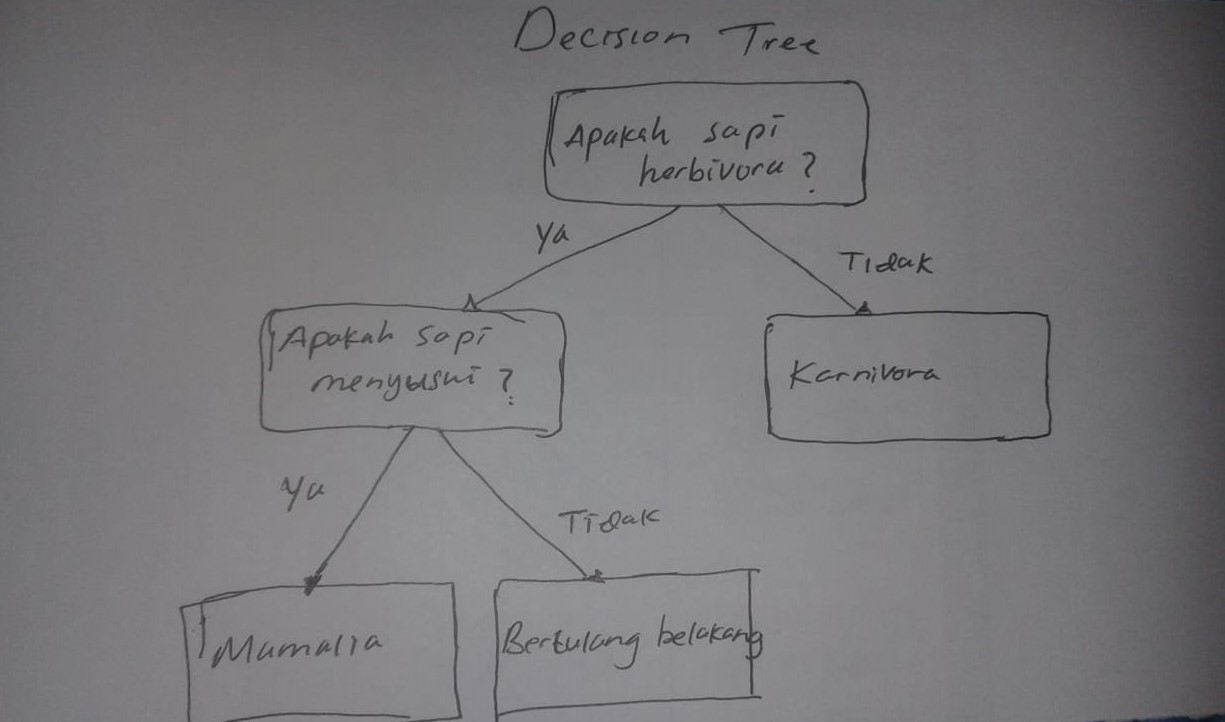
\includegraphics[width=1\textwidth]{figures/AIP/6.JPEG}}
		\caption{Decision Tree.}
		\label{6}
		\end{figure}

\end{enumerate}

\subsection{Gain Dan Entropi}
\begin{enumerate}
\item Gain adalah pengurangan yang diharapkan dalam enthropy. Dalam mechine learning, gain dapat digunakan untuk menentukan sebuah urutan atribut atau memperkecil atribut yang telah dipilih. Urutan ini akan membentuk decision tree. atribut gain dipilih yang paling besar.

\item Entropi adalah ukuran ketidakpastian sebuah variabel acak sehingga dapat di artikan entropi adalah ukuran ketidakpastian dari sebuah atribut.

\subitem Ilustrasi dari gain dan entropi adalah bagaimana kita memprediksi jenis kelamin berdasarkan atributnya, perhatikan pada gambar \ref{7}

		\begin{figure}[ht]
		\centerline{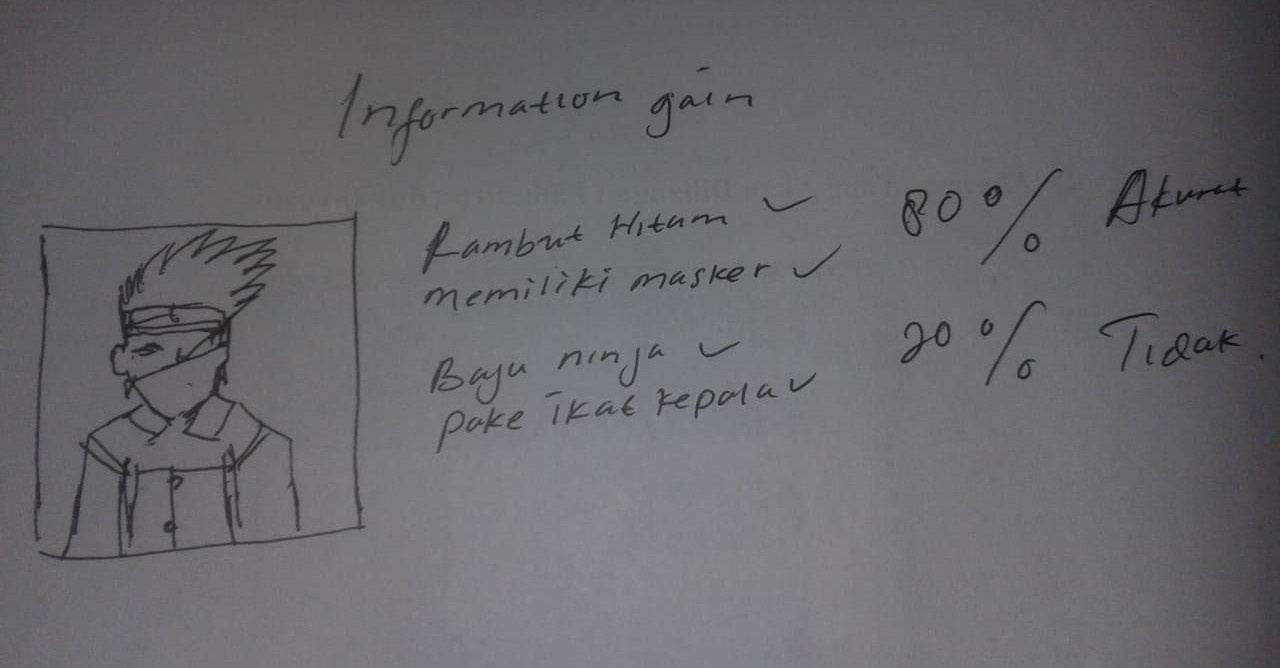
\includegraphics[width=1\textwidth]{figures/AIP/7.JPEG}}
		\caption{Gain Dan Entropi.}
		\label{7}
		\end{figure}
\end{enumerate}

\section{Aip Suprapto Munari/1164063}
\subsection{Scikit-learn}
Penyelesaian Tugas Harian 4 
\begin{itemize}
\item Pembahasan Codingan Dan Hasilnya
\begin{enumerate}
\item Gambar Pertama :
\par Penjelasan : Pada baris pertama itu merupakan import library sebagai variabel siomay  Dan pada baris kedua variabel siomay membaca file csv nya. Dan pada baris ketiga merupakan hasilnya yaitu 395.

\par
\begin{itemize}
\par
\item Hasil  Gambar Pertama :
\par

\begin{figure}[ht]
\centering
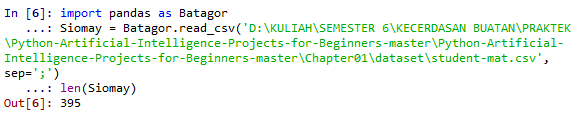
\includegraphics[scale=0.6]{figures/AIP/jd1.PNG}
\caption{ Gambar pertama}
\label{1}
\end{figure}

\par
\end{itemize}
\item  Gambar Kedua :
\par Penjelasan : Variabel Siomay mengimplementasikan baris 1, dari baris G1, G2, G3. Dan variabel siomay akan ngedrop kolom G1, G2,G3. Dan hasilnya akan seperti gambar di out nya.
\par 
\begin{itemize}
\par
\item Hasil Gambar Kedua :

\begin{figure}[ht]
\centering
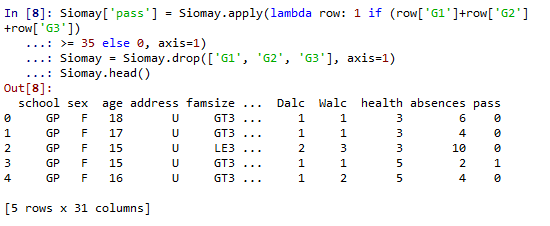
\includegraphics[scale=0.7]{figures/AIP/jd2.PNG}
\caption{Gambar kedua}
\label{2}
\end{figure}

\end{itemize}
\par
\item  Gambar Ketiga :
\par Penjelasan : Variabel Siomay mengambil atau get data dari dalam kolom. Atau yang tulisan berwarna hijau. Dan kemudian ditampilkan pada outputan yang dibawah atau menampilkan hasilnya.
\par 
\begin{itemize}
\par
\item Hasil  Gambar Ketiga :

\begin{figure}[ht]
\centering
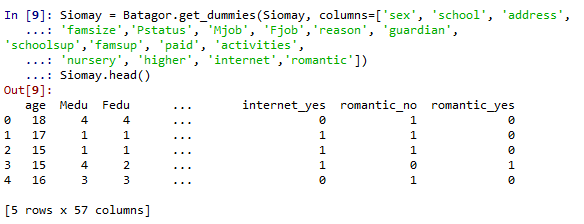
\includegraphics[scale=0.5]{figures/AIP/jd3.PNG}
\caption{ Gambar Ketiga}
\label{3}
\end{figure}

\end{itemize}
\par
\item  Gambar Keempat :
\par Penjelasan : Penejelasan pada gambar keempat adalah variabel Siomay akan menampilkan sampel data dari 500 training data dan 500 tetsing data. Kemudia data akan dicetak atau di print dari training data dan testing data.
\par 
\begin{itemize}
\par
\item Hasil  Gambar Keempat :

\begin{figure}[ht]
\centering
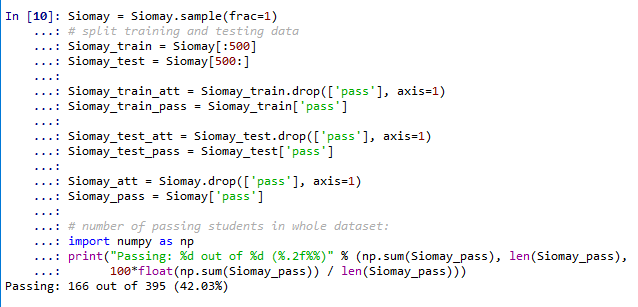
\includegraphics[scale=0.5]{figures/AIP/jd4.PNG}
\caption{ Gambar Keempat}
\label{4}
\end{figure}

\end{itemize}
\par
\item  Gambar Kelima :
\par Penjelasan : Pada gambar tersebut variabel hanya melakukan pengetesan/pengecekan terhadap decission tree. Apabila decission tree nya benar maka kodingan tidak eror tapi jika tidak benar maka kodingan akan error. 
\par 
\begin{itemize}
\par
\item Hasil  Gambar Kelima :

\begin{figure}[ht]
\centering
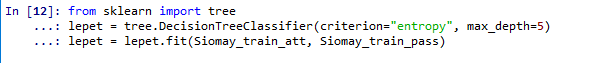
\includegraphics[scale=0.7]{figures/AIP/jd5.PNG}
\caption{ Gambar Kelima}
\label{5}
\end{figure}


\end{itemize}
\item  Gambar Keenam :
\par Penjelasan : Pada gambar nomor 6, tejadi kesalah error yaitu pada import graphivz.
\par 
\begin{itemize}
\par
\item Hasil  Gambar Keenam :

\begin{figure}[ht]
\centering
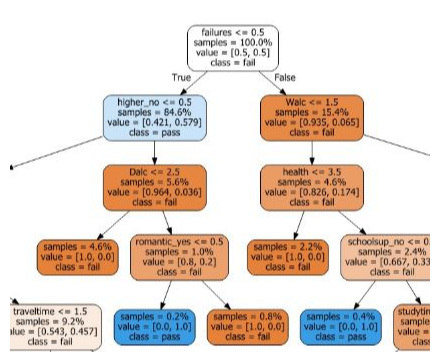
\includegraphics[scale=0.4]{figures/AIP/jd13.PNG}
\caption{ Gambar Keenam}
\label{13}
\end{figure}


\end{itemize}
\item  Gambar Ketujuh :
\par Penjelasan : Pada gambar 7 akan menampilkan yang terdapat pada Library Graphviz, apabila benar akan menampilkan hasil output seperti yang terdapat pada gambar atau kalau pengujian gagal akan terdapat error.
\par 
\begin{itemize}
\par
\item Hasil  Gambar Ketujuh :

\begin{figure}[ht]
\centering
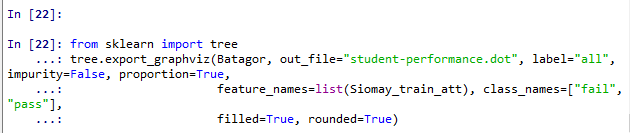
\includegraphics[scale=0.6]{figures/AIP/jd7.PNG}
\caption{ Gambar Ketujuh}
\label{7}
\end{figure}


\end{itemize}
\item  Gambar Kedelapan :
\par Penjelasan : Pada gambar 8 menampilkan hasil perhitungan dari kedua parameter yang terdapat pada code tersebut.
\par 
\begin{itemize}
\par
\item Hasil  Gambar Kedelapan :

\begin{figure}[ht]
\centering
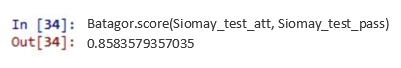
\includegraphics[scale=0.8]{figures/AIP/jd8.PNG}
\caption{ Gambar Kedelapan}
\label{8}
\end{figure}


\end{itemize}
\item  Gambar Kesembilan:
\par Penjelasan : Pada gambar 9, kodingan teresbut mnedefinisikan library sklearn model selection dan import cross val score. Dan kemudian variabel scores mengeksekusi fungsi cross val score(Batagor, Siomay att, Siomay pass, cv=5). Kemudian akan menampilkan nilai dari fungsi akurasinya.
\par 
\begin{itemize}
\par
\item Hasil  Gambar Kesembilan :

\begin{figure}[ht]
\centering
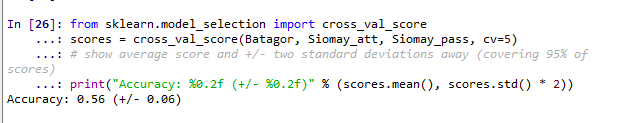
\includegraphics[scale=0.4]{figures/AIP/jd9.PNG}
\caption{ Gambar Kesembilan}
\label{9}
\end{figure}


\end{itemize}
\item  Gambar Kesepuluh :
\par Penjelasan : Pada gambar di atas kodingan nya berfungsi untuk menampilkan hasil dari fungsi Max Depth dan Accuraccy dari dari Decission Tree. Yaitu menmpilkan data dari angka 1-20. 
\par 
\begin{itemize}
\par
\item Hasil  Gambar Kesepuluh :

\begin{figure}[ht]
\centering
\includegraphics[scale=0.9]{figures/AIP/jd10.PNG}
\caption{ Gambar Kesepuluh}
\label{10}
\end{figure}


\end{itemize}
\item  Gambar Kesebelas :
\par Penjelasan : Pada gambar 11 dijelaskan bahwa variable scores akan menampilkan atau mendefinisikan nilai dari variabel score yang mana isi dari variable score yaitu Batagor, Siomay att, Siomay pass, cv=5. Yang mana hasil tampilan dari kodingannya adalah outputan seperti gambar 11.
\par 
\begin{itemize}
\par
\item Hasil  Gambar Kesebelas :

\begin{figure}[ht]
\centering
\includegraphics[scale=0.5]{figures/AIP/jd11.PNG}
\caption{ Gambar Kesebelas}
\label{11}
\end{figure}


\end{itemize}
\item  Gambar Keduabelas :
\par Penjelasan : Pada gambar di atas dijelaskan bahwa pada library matplotlib akan menampilkan gambar grafik pada gambar 12 dari eksekusi fungsi ax.errorbar.
\par 
\begin{itemize}
\par
\item Hasil  Gambar Keduabelas :

\begin{figure}[ht]
\centering
\includegraphics[scale=0.5]{figures/AIP/jd12.PNG}
\caption{ Gambar Keduabelas}
\label{12}
\end{figure}


\end{itemize}
\end{enumerate}

\end{itemize}

\subsection{Penanganan Error}
\begin{enumerate}
\item Skrinsut Error
\begin{figure}[ht]
\centering
\includegraphics[scale=0.5]{figures/AIP/jd6.PNG}
\caption{ Gambar Ketigabelas}
\label{6}
\end{figure}
\item Kode Error dan Jenis Errornya
\par Kode Error: "Import Graphiz" dan "ModulNotFoundError". 
\par Jenis Error: Pada Grafik
\item Penanganan
\par Melakukan install ulang pada graphiz

\end{enumerate}



\section{Andi Aslam/1164064}
\subsection{Binary Clasification beserta gambar}
\begin{enumerate}
\item Output aktual dari banyak algoritma klasifikasi biner adalah skor prediksi. Skor menunjukkan kepastian sistem bahwa pengamatan yang diberikan adalah milik kelas positif. Untuk membuat keputusan tentang apakah pengamatan harus diklasifikasikan sebagai positif atau negatif, sebagai konsumen skor ini, Anda akan menginterpretasikan skor dengan memilih ambang klasifikasi (cut-off) dan membandingkan skor dengan itu. Setiap pengamatan dengan skor lebih tinggi dari ambang kemudian diprediksi sebagai kelas positif dan skor lebih rendah dari ambang diprediksi sebagai kelas negatif.

\begin{figure}[ht]
\centering
\includegraphics[scale=0.5]{figures/andi/clustring1.png}
\caption{Binary Clasification}
\label{contoh}
\end{figure}
\end{enumerate}

\subsection{supervised learning dan unsupervised learning dan clustering dengan ilustrasi gambar}
\begin{enumerate}
\item Supervised learning adalah tugas pembelajaran mesin untuk mempelajari suatu fungsi yang memetakan input ke output berdasarkan contoh pasangan input-output. Ini menyimpulkan fungsi dari data pelatihan berlabel yang terdiri dari serangkaian contoh pelatihan. Dalam pembelajaran yang diawasi, setiap contoh adalah pasangan yang terdiri dari objek input (biasanya vektor) dan nilai output yang diinginkan (juga disebut sinyal pengawas). Algoritma pembelajaran yang diawasi menganalisis data pelatihan dan menghasilkan fungsi yang disimpulkan, yang dapat digunakan untuk memetakan contoh-contoh baru. Skenario optimal akan memungkinkan algoritma menentukan label kelas dengan benar untuk instance yang tidak terlihat. Ini membutuhkan algoritma pembelajaran untuk menggeneralisasi dari data pelatihan untuk situasi yang tidak terlihat dengan cara yang "masuk akal" (lihat bias induktif).
\item Unsupervised learning adalah istilah yang digunakan untuk pembelajaran bahasa Ibrani, yang terkait dengan pembelajaran tanpa guru, juga dikenal sebagai organisasi mandiri dan metode pemodelan kepadatan probabilitas input. Analisis cluster sebagai cabang pembelajaran mesin yang mengelompokkan data yang belum diberi label, diklasifikasikan atau dikategorikan. Alih-alih menanggapi umpan balik, analisis klaster mengidentifikasi kesamaan dalam data dan bereaksi berdasarkan ada tidaknya kesamaan di setiap potongan data baru. BErikut merupakan contoh Unsupervised Learning dengan Gaussian mixture models.


\begin{figure}[ht]
\centering
\includegraphics[scale=1]{figures/andi/ilustrasi2.PNG}
\caption{Supervised Learning}
\label{ilustrasi gambar}
\end{figure}
\end{enumerate}

\subsection{evaluasi dan akurasi dari buku dan disertai ilustrasi contoh dengan gambar}
\begin{enumerate}
\item Evaluasi adalah tentang  bagaimana kita dapat mengevaluasi seberapa baik model bekerja dengan mengukur akurasinya. Dan akurasi akan didefinisikan sebagai persentase kasus yang diklasifikasikan dengan benar. Kita dapat menganalisis kesalahan yang dibuat oleh model, atau tingkat kebingungannya, menggunakan matriks kebingungan. Matriks kebingungan mengacu pada kebingungan dalam model, tetapi matriks kebingungan ini bisa menjadi sedikit sulit untuk dipahami ketika mereka menjadi sangat besar.
\begin{figure}[ht]
\centering
\includegraphics[scale=1]{figures/andi/no3.PNG}
\caption{ Evaluasi dan Akurasi}
\label{contoh}
\end{figure}
\end{enumerate}

\subsection{ bagaimana cara membuat dan membaca confusion matrix, buat confusion matrix }
\begin{enumerate}
\item  Confusion matrix :
\begin{itemize}
\item 1)	Tentukan pokok permasalahan dan atributanya, misal gaji dan listik.
\item 2)	Buat pohon keputusan
\item 3)	Lalu data testingnya
\item 4)	Lalu mencari nilai a, b, c, dan d. Semisal a = 5, b = 1, c = 1, dan d = 3.
\item 5)	Selanjutnya mencari nilai recall, precision, accuracy, serta dan error rate.
\end{itemize}
\item Berikut adalah contoh dari confusion matrix :
\begin{itemize}
\item Recall =3/(1+3) = 0,75
\item Precision = 3/(1+3) = 0,75
\item Accuracy =(5+3)/(5+1+1+3) = 0,8
\item Error Rate =(1+1)/(5+1+1+3) = 0,2
\end{itemize}
\end{enumerate}

\subsection{bagaimana K-fold cross validation bekerja dengan gambar ilustrasi}
\begin{enumerate}
\item Cara kerja K-fold cross validation :
\begin{itemize}
\item 1)	Total instance dibagi menjadi N bagian.
\item 2)	Fold yang pertama adalah bagian pertama menjadi data uji (testing data) dan sisanya menjadi training data.
\item 3)	Lalu hitung akurasi berdasarkan porsi data tersebut dengan menggunakan persamaan.
\item 4)	Fold yang ke dua adalah bagian ke dua menjadi data uji (testing data) dan sisanya training data. 
\item 5)	Kemudian hitung akurasi berdasarkan porsi data tersebut.
\item 6)	Dan seterusnya hingga habis mencapai fold ke-K.
\item 7)	Terakhir hitung rata-rata akurasi K buah.
\end{itemize}
\begin{figure}[ht]
\centering
\includegraphics[scale=1]{figures/andi/no5.PNG}
\caption{K-fold cross validation}
\label{contoh}
\end{figure}
\end{enumerate}

\subsection{decision tree dengan gambar ilustrasi}
\begin{enumerate}
\item Decision Tree dalah metode pembelajaran yang diawasi non-parametrik yang digunakan untuk klasifikasi dan regresi. Tujuannya adalah untuk membuat model yang memprediksi nilai variabel target dengan mempelajari aturan keputusan sederhana yang disimpulkan dari fitur data.\\
Misalnya, dalam contoh di bawah ini, decision tree belajar dari data untuk memperkirakan kurva sinus dengan seperangkat aturan keputusan if-then-else. Semakin dalam pohon, semakin rumit aturan keputusan dan semakin bugar modelnya.
\begin{figure}[ht]
\centering
\includegraphics[scale=0.5]{figures/andi/tree.jpg}
\caption{Decision Tree}
\label{contoh}
\end{figure}
\end{enumerate}

\subsection{Information Gain dan entropi dengan gambar ilustrasi}
\begin{enumerate}
\item Information gain didasarkan pada penurunan entropi setelah dataset dibagi pada atribut. Membangun decision tree adalah semua tentang menemukan atribut yang mengembalikan perolehan informasi tertinggi (mis., Cabang yang paling homogen).
\item Entropi adalah ukuran keacakan dalam informasi yang sedang diproses. Semakin tinggi entropi, semakin sulit untuk menarik kesimpulan dari informasi itu. Membalik koin adalah contoh tindakan yang memberikan informasi yang acak. Untuk koin yang tidak memiliki afinitas untuk kepala atau ekor, hasil dari sejumlah lemparan sulit diprediksi. Mengapa? Karena tidak ada hubungan antara membalik dan hasilnya. Inilah inti dari entropi.
\begin{figure}[ht]
\centering
\includegraphics[scale=0.5]{figures/andi/no7.PNG}
\caption{Entropi}
\label{contoh}
\end{figure}
\end{enumerate}


\section{Same Topics}
Cite every latest journal with same topic
\subsection{Topic 1}
cite for first topic

\subsection{Topic 2}
if you have two topics you can include here to


\section{Same Method}
write and cite latest journal with same method

\subsection{Method 1}
cite and paraphrase method 1

\subsection{Method 2}
cite and paraphrase method 2 if you have more method please add new subsection.




 
\chapter{Methods}

\section{The data}
PLease tell where is the data come from, a little brief of company can be put here.

\section{Method 1}
Definition, steps, algoritm or equation of method 1 and how to apply into your data
\section{Method 2}
Definition, steps, algoritm or equation of method 2 and how to apply into your data


\section{Aip Suprapto Munari/1164063}
\subsection{Teori}
Tugas Harian 5 
\begin{enumerate}
\item Random Forest Dan Ilustrasi Gambarnya
\begin{itemize}
\item Pengertian Random Forest:
\par Random Forest adalah suatu algoritma yang digunakan pada klasifikasi data dalam jumlah yang besar. Klasifikasi random forest dilakukan melalui penggabungan pohon  dengan melakukan training pada sampel data yang dimiliki. Penggunaan pohon (tree) yang semakin banyak akan mempengaruhi akurasi yang akan didapatkan menjadi lebih baik. Penentuan klasifikasi dengan random forest diambil berdasarkan hasil voting dari pohon yang terbentuk. Pemenang dari pohon yang terbentuk ditentukan dengan vote terbanyak. 
\par Pembangunan pohon  pada random forest sampai dengan mencapai ukuran maksimum dari pohon data. Akan tetapi,pembangunan pohon random foresttidak dilakukan pemangkasan  yang merupakan sebuah metode untuk mengurangi kompleksitas ruang.
\item Ilustrasi Gambar Random Forest :
\par

\begin{figure}[ht]
\centering
\includegraphics[scale=0.9]{figures/AIP/asm1.PNG}
\caption{Random Forest}
\label{contoh}
\end{figure}

\par
\end{itemize}

\item Cara Membaca Dataset

Berikut adalah cara membaca dataset :
\begin{itemize}
\item Buka Anaconda Navigator lalu jalankan Syder, kemudian import libraries yang dibutuhkan.
\item Masukkan kode python untuk membaca file csv, lalu jalankan

\begin{figure}[ht]
\centering
\includegraphics[scale=0.5]{figures/AIP/y1.PNG}
\caption{(b)}
\label{contoh}
\end{figure}
\par (c) Maka pada window console akan menampilkan pesan berikut :
\begin{figure}[ht]
\centering
\includegraphics[scale=0.9]{figures/AIP/y2.PNG}
\caption{(c)}
\label{contoh}
\end{figure}
\par (d) Dari explorer dapat terlihat dataset yang terimport.
\begin{figure}[ht]
\centering
\includegraphics[scale=0.6]{figures/AIP/y3.PNG}
\caption{(d)}
\label{contoh}
\end{figure}
\par (e) Lalu klik dataset cell, maka akan muncul seperti berikut :
\begin{figure}[ht]
\centering
\includegraphics[scale=0.9]{figures/AIP/y4.PNG}
\caption{(e)}
\label{contoh}
\end{figure}
\par (f) Seperti yang terlihat pada gambar tersebut dataset ini memiliki Kolom Country, Age, dan Salary sebagai independent variable-nya dan kolom Purchased sebagai dependent variable-nya.
\par (g) Selanjutnya buat 2 matrix of features yang berisi values dari independent variable dan dependent variable.
\par (h) Lalu tuliskan perintah berikut :
\begin{figure}[ht]
\centering
\includegraphics[scale=0.9]{figures/AIP/y5.PNG}
\caption{(h)}
\label{contoh}
\end{figure}
\par (i) Perintah yang telah dibuat di atas akan membuat sebuah global environment baru dan muncul dataset.
\par (j) Klik dataset tersebut maka muncul tabel berisi dataset.

\end{itemize}

\item Cross Validation
\begin{itemize}
\item Pengertian Cross Validation : 
\par Cross Validation adalah sebuah teknik validasi model yang digunakan untuk menilai bagaimana hasil analisis statistik akan digeneralisasi ke kumpulan data independen. Cross validation digunakan dengan tujuan prediksi, dan bila kita ingin memperkirakan seberapa akurat model model prediksi yang dilakukan dalam sebuah praktek. Tujuan dari cross validation yaitu untuk mendefinisikan dataset guna menguju dalam fase pelatihan untuk membatasi masalah seperti overfitting dan underfitting serta mendapatkan wawasan tentang bagaimana model akan digeneralisasikan ke set data independen.

\par
\end{itemize}
\item Penjelasan / Maksud Dari Score pada :
\begin{itemize}
\item Random forest ( 44\% )
\par Maksud arti score 44\%  pada random forest adalah hasil dari akurasi. Yang menggunakan 5 buah atribut yaitu dari 5 baris pertama dari set pelatihan yang akan memprediksi spesies 10, 28, 156, 10 dan 43.
\par

\item Decision Tree ( 27\% )
\par Maksud arti score 27\% pada decission tree adalah presentasi hasil dari perhitungan dataset. Dari set tentang burung pipit. Confusion matrix memberi tau hal-hal yang diharapkan, artinya, butrung-burung yang terlihat mirip saling bingung satu sama lain. 
\par

\item SVM ( 29\% )
\par Maksud arti score 29\% dari SVM adalah hasil pendekatan jaringan saraf. Di sini, akurasinya adalah 27\%, yang kurang dari akurasi 44\% sebelumnya. Oleh karena itu, dessicion tree menjadi  lebih buruk. Jika kita menggunakan Support Vector Machine (SVM), yang merupakan neural pendekatan jaringan, outputnya 29\%. Jadi 29\% pada SVM merupakan hasil otputannya.
\par
\par Hasil tersebut didapat dari hasil valdasi silang untuk memastikan bahwa membagi training test dengan cara yang berbeda. Sehingga didapat outputnya 44\% untuk hutan acak, 27\% untuk pohon keputusan, dan 29\% untuk SVM.
\par
\end{itemize}

\par
\item Confusion Matrix Dan Ilustrasinya
\begin{itemize}
\item Cara Membaca Confusion Matrix :
\par Perhitungan confusion matrix adalah sebagai berikut, akan saya beri contoh sederhana yaitu pengambilan keputusan untuk mendapatkan bantuan beasiswa. Saya menggunakan dua atribut, yaitu rekening listrik dan gaji. Yang pertama kita lakukan yaitu mencari 4 nilai yaitu a,b,c, dan d:
\par a= 4
\par b= 1
\par c= 1
\par d= 2
\par Kemudian kita dapat mencari nilai Recall, Precision, accuracy dan Error Rate
\par Recall =2/(1+2) = 0,66
\par Precision = 2/(1+2) = 0,66
\par Accuracy =(4+2)/(4+1+1+2) = 0,75
\par Error Rate =(1+1)/(4+1+1+4) = 0,2
\par Ilustrasi Confusion Matrix :
\par
\begin{figure}[ht]
\centering
\includegraphics[scale=1]{figures/AIP/asm3.PNG}
\caption{Confussion Matrik}
\label{contoh}
\end{figure}
\end{itemize}

\par
\par
\item Voting Random Forest Dan Ilustrasi Gambarnya.
\par
\begin{itemize}
\item Pengertian Voting pada Random Forest	:
\par Metode ensemble dapat mencapai akurasi tinggi dengan membangun beberapa pengklasifikasi dan menjalankan
masing-masing secara mandiri. Ketika classifier membuat sebuah keputusan, kamu dapat memanfaatkan yang terbaik
keputusan umum dan rata-rata. Jika kita menggunakan metode yang paling umum, itu disebut voting.
\item Ilustrasi Gambar Voting Random Forest :
\begin{figure}[ht]
\centering
\includegraphics[scale=1]{figures/AIP/asm2.PNG}
\caption{Voting Random forest}
\label{contoh}
\end{figure}
\end{itemize}
\end{enumerate}

section{Andi Muhammad Aslam/1164064}
\begin{enumerate}

\item Random Forest merupakan algoritma yang digunakan terhadapap klasifikasi data dalam jumlah yang besar. Klasifikasi pada random forest dilakukan dengan penggabungan dicision tree dengan melakukan training terhadap sempel data yang dimiliki. Pembentukan decision tree menggunakan sample data berupa variable secara acak lalu menjalankan klasifikasi pada semua tree yang terbentuk. Random forest berupa Decision Tree agar dapat melakukan proses seleksi. Decision tree yang di buat dibagi secara strategis dari data pada kelas yang sama. Pemecahan digunakan untuk membagi data berdasarkan jenis atribut yang digunakan..  \ref{Andi}

\begin{figure}[ht]
	\centerline{\includegraphics[width=1\textwidth]{figures/andi/decision tree.jpg}}
	\caption{Random Forest.}
	\label{contoh}
	\end{figure}

\item Download dataset terdahulu kemudian buka software spyder untuk melihat isi dataset. Data yang di download berupa extensi file bernama .txt yang terdapat class dari field. Contohnya pada data jenis burung memiliki file index dan angka, dimana index berisi angka yang memiliki makna berupa jenis burung atau bahkan nama burung sedangkan field memiliki isi nilai berupa 0 dan 1 yang dimana sifatnya boolean, Ya dan Tidak. Hal ini dikarenakan komputer hanya dapat membaca bilangan biner maka dari itu field yang di isikan berupa angka. Artinya angka 0 berarti tidak dan angka 1 berarti Ya.

\item Cross validation adalah metode statistik yang digunakan untuk memperkirakan keterampilan model pembelajaran mesin. Ini biasanya digunakan dalam pembelajaran mesin yang diterapkan untuk membandingkan dan memilih model untuk masalah pemodelan prediktif yang diberikan karena mudah dipahami, mudah diimplementasikan, dan menghasilkan estimasi keterampilan yang umumnya memiliki bias lebih rendah daripada metode lainnya.

\item Penjelasan Score
	\begin{itemize}
		\item Pada score 44\% pada random forest berupa hasil akurasi.
		\item Pada score 27\% pada decision tree adalah presentasi hasil dari perhitungan dataset.
		\item Pada  score 29\% dari SVM adalah hasil pendekatan neural network.
		\item Hasil tersebut didapat dari hasil valdasi silang untuk memastikan bahwa membagi  training test dengan cara yang berbeda. Sehingga dapat diketahui hasi output yaitu 44\% untuk hutan, 27\% untuk pohon keputusan, dan 29\% untuk SVM.
	\end{itemize}

\item Untuk membaca confusion matriks dapat menggunakan source code berikut :
	\begin{verbatim}
		import numpy as np
		np.set_printoptions(precision=2)
		plt.figure(figsize=(60,60), dpi=300)
		plot_confusion_matrix(cm, classes=birds, normalize=True)
		plt.show()
	\end{verbatim}

Dimana numpy dapat mengelola data yang berhubungan pada matrix. Pada perintah code tersebut digunakan dalam melakukan read pada dataset burung dengan menggunakan metode confusion matrix. Dalam confusion matrix memiliki 4 istilah yaitu True Positive yang merupakan data posotif yang terditeksi benar, True Negatif yang merupakan data negatif akan tetapi terditeksi benar, False Positif merupakan data negatif namun terditeksi sebagai data positif, False Negatif merupakan data posotif namun terditeksi sebagai data negatif. Adapun contoh hasil read dataset menggunakan confusion matrix dapat dilihat pada figure \ref{Andi}

\item Untuk mengetahui confusion matriks kita dapat melihat contoh klasifikasi dari biner berikut ini :
	\begin{figure}[ht]
	\centerline{\includegraphics[width=1\textwidth]{figures/andi/CM.PNG}}
	\caption{Tabel Confusion Matriks}
	\label{contoh}
	\end{figure}
\item Voting merupakan proses pemilihan dari tree yang dimana akan dimunculkan hasilnya dan disimpulkan menjadi informasi yang pasti.
	\begin{figure}[ht]
	\centerline{\includegraphics[width=1\textwidth]{figures/andi/Voting.PNG}}
	\caption{Voting}
	\label{Contoh Voting}
	\end{figure}

Pada figure Voting terdapat Decision Tree yang terbagi menjadi 3 Branch yaitu tree 1, tree 2, dan tree 3. Pada tree tersebut akan dilakukan proses voting. Pada  masing-masing tree tersebut memiliki data-data yang berbeda, yang di mana data tersebut akan di pilih dengan cara voting. Hasli voting dari setiap tree tersebut menunjukkan data pada setiap tree, Di sini kita dapat menghitung akurasi dengan menambahkan angka secara diagonal, sehingga ini semua adalah contoh yang diklasifikasikan dengan benar, dan membagi jumlah tersebut dengan jumlah semua angka dalam matriks.

\end{enumerate}
\chapter{Experiment and Result}
brief of experiment and result.
\section{Experiment}
Please tell how the experiment conducted from method.

\section{Result}
Please provide the result of experiment

\section{Aip Suprapto Munari/1164063}

\subsection{Teori}
\begin{enumerate}
\item Klasifikasi teks
	\par Klasifikasi teks atau kategorisasi teks merupakan proses yang secara otomatis menempatkan dokumen teks ke dalam suatu kategori berdasarkan isi dari teks tersebut. 
	\begin{figure}[ht]
		\centering
		\includegraphics[scale=0.5]{figures/AIP/b1.PNG}
		\caption{Aip-Klasifikasi teks}
		\label{contoh}
	\end{figure}
	
\item Klasifikasi Bunga tidak dapat penggunakan machine learning
	\par Dikarenakan masalah dari input yang serupa namun output yang berbeda ‘noise’, yang dimaksud dengan noise adalah contoh pada output yang direkam bukan seperti perkiraan.
	\begin{figure}[ht]
		\centering
		\includegraphics[scale=0.5]{figures/AIP/b2.PNG}
		\caption{Aip-Klasifikasi bunga}
		\label{contoh}
	\end{figure}

\item Teknik pembelajaran mesin pada teks YouTube
	\par Teknik Machine Learning pada YouTube memperhatikan apa saja yang menarik perhatian para penggunanya. Ketika kita sedang menonton di YouTube, pada sebelah kanan terdapat 'Up Next' yang menampilkan beberapa video serupa yang sedang ditonton. Dan ketika mengklik salah satu video dari baris tersebut, maka YouTube akan mengingatnya dan menggunakan kata yang tertera sebagai referensi.
	\begin{figure}[ht]
		\centering
		\includegraphics[scale=0.5]{figures/AIP/b3.PNG}
		\caption{Aip-Teknik YouTube}
		\label{contoh}
	\end{figure}

\item Vectorisasi Data
	\begin{itemize}
		\item Vectorisasi Data merupakan pemecahan serta pembagian data kemudian dilakukan perhitungan datanya.
	\end{itemize}
	
\item Bag of word
	\par Bag of Words adalah metode untuk mengekstraksi fitur dari dokumen teks.
	\begin{figure}[ht]
		\centering
		\includegraphics[scale=0.5]{figures/AIP/b4.PNG}
		\caption{Aip-Bag of Word}
		\label{contoh}
	\end{figure}
	
\item TF-IDF
	\par TF-IDF merupakan istilah beberapa frekuensi dokumen terbalik, adalah ukuran penilaian yang banyak digunakan dalam pengambilan informasi (IR) atau peringkasan. 
	\begin{figure}[ht]
		\centering
		\includegraphics[scale=0.5]{figures/AIP/b5.PNG}
		\caption{Aip-TF IDF}
		\label{contoh}
	\end{figure}
\end{enumerate}
\chapter{Conclusion}
brief of conclusion

\section{Conclusion of Problems}
Tell about solving the problem

\section{Conclusion of Method}
Tell about solving using method

\section{Conclusion of Experiment}
Tell about solving in the experiment

\section{Conclusion of Result}
tell about result for purpose of this research.

\section{Andi Muh Aslam/1164064}
\subsection{Teori}
\begin{enumerate}
\item Jelaskan Kenapa Kata-Kata harus dilakukan vektorisasi lengkapi dengan ilustrasi gambar.
\subitem Kata-kata harus dilakukan vektorisasi untuk mengukur nilai kemunculan suatu kata agar dapat di prediksi atau untuk menentukan bobot suatu kata.
\par Untuk ilustrasinya dapat dilihat pada gambar
\begin{figure}[ht]
	\centerline{\includegraphics[width=1\textwidth]{figures/andi/L1.PNG}}
	\caption{Ilustrasi Soal No.1}
\end{figure}

\item Jelaskan Mengapa dimensi dari vektor dataset google bisa mencapai 300 lengkapi dengan ilustrasi gambar.
\subitem Dimensi dari vektor dataset google dapat mencapai 300 karena dimensi pada vektor agar dapat membandingkan bobot dari kata tersebut, misalkan terdapat kata Jaket dan Tas pada data set google setiap kata tersebut di buat dimensi vektor senilai 300 kata Jaket dan 300 kata Tas, agar dapat membandingkan bobot dari kesamaan kata Jaket dan Tas. 
\par Untuk ilustrasinya dapat dilihat pada gambar 
\begin{figure}[ht]
	\centerline{\includegraphics[width=1\textwidth]{figures/andi/L2.PNG}}
	\caption{Ilustrasi Soal No. 2}
	
\end{figure}

\item Jelaskan Konsep vektorisasi untuk kata . dilengkapi dengan ilustrasi atau gambar.
\subitem Konsep dari vektorisasi kata yaitu agar dapat mengetahui kata tengah pada kalimat utama, Contoh ( Subscribe channel ini dan Like yah Guys ). Kata tengah dari contoh tersebut merupakan (dan) yang memiliki bobot sebagai kata tengah dari kalimat. Hal ini sangat berkaitan dengan dimensi vektor pada dataset google karena memiliki nilai atau bobot kata tengah.
\par Untuk ilustrasinya dapat dilihat pada gambar \begin{figure}[ht]
	\centerline{\includegraphics[width=1\textwidth]{figures/andi/L3.PNG}}
	\caption{Ilustrasi Soal No. 3}
	
\end{figure}
\item Jelaskan Konsep vektorisasi untuk dokumen. dilengkapi dengan ilustrasi atau gambar.
\subitem Konsep vektorisasi pada dokumen mesin akan membaca kata-kata terlebih dahulu pada semua kalimat yang ada di dalam dokumen dan nanti kalimat yg ada di dalam dokumen akan dipecah menjadi kata-kata.
\par Untuk ilustrasinya dapat dilihat pada gambar 
\begin{figure}[ht]
	\centerline{\includegraphics[width=1\textwidth]{figures/andi/L4.PNG}}
	\caption{Ilustrasi Soal No. 4}
	
\end{figure}

\item Jelaskan apa mean dan standar deviasi, lengkapi dengan iludtrasi atau gambar.
\subitem Mean merupakan nilai rata-rata yang tingkat akurasinya tinggi atau nilai tersebut sering munucul. Standar deviasi mengukur bagaimana nilai-nilai data tersebar. Bisa juga didefinisikan sebagai, rata-rata jarak penyimpangan titik-titik data diukur dari nilai rata-rata data tersebut.
\par Untuk ilustrasinya dapat dilihat pada gambar 
\begin{figure}[ht]
	\centerline{\includegraphics[width=1\textwidth]{figures/andi/L5.PNG}}
	\caption{Ilustrasi Soal No. 5}
	
\end{figure}

\item Jelaskan Apa itu Skip-Gram sertakan contoh ilustrasi.
\subitem Skip-Gram yaitu dimana kata tengah menjadi acuan terhadap kata kata pelengkap dalam suatu kalimat.
\par Untuk ilustrasinya dapat dilihat pada gambar 
\begin{figure}[ht]
	\centerline{\includegraphics[width=1\textwidth]{figures/andi/L6.PNG}}
	\caption{Ilustrasi Soal No. 6}
	
\end{figure}
\end{enumerate}

\subsection{Praktek Program}
\begin{enumerate}
\item Cobalah dataset google, dan jelaskan vektor dari kata love, faith, fall, sick, clear, shine, bag, car, wash, motor, cycle dan cobalah untuk melakukan perbandingan similirati dari masing-masing kata tersebut. Jelaskan arti dari outputan similaritas.
\subitem Output source code dibawah akan memunculkan data vektor untuk kata love. bahwa vektor memiliki array sebanyak 300 dimensi. Hasil pada source code tersebut dapat dilihat pada gambar.
\begin{verbatim}
gmodel['love']
\end{verbatim}
\begin{figure}[ht]
	\centerline{\includegraphics[width=1\textwidth]{figures/andi/E1.PNG}}
	\caption{Love}
	\label{c5_7}
\end{figure}
\subitem Output source code dibawah akan memunculkan data vektor untuk kata faith. bahwa vektor memiliki array sebanyak 300 dimensi. Hasil pada source code tersebut dapat dilihat pada gambar \ref{c5_8}.
\begin{verbatim}
gmodel['faith']
\end{verbatim}
\begin{figure}[ht]
	\centerline{\includegraphics[width=1\textwidth]{figures/andi/E2.PNG}}
	\caption{Faith}
	\label{c5_8}
\end{figure}
\subitem Output source code dibawah akan memunculkan data vektor untuk kata fall. bahwa vektor memiliki array sebanyak 300 dimensi. Hasil pada source code tersebut dapat dilihat pada gambar \ref{c5_9}.
\begin{verbatim}
gmodel['fall']
\end{verbatim}
\begin{figure}[ht]
	\centerline{\includegraphics[width=1\textwidth]{figures/andi/E3.PNG}}
	\caption{Fall}
	\label{c5_9}
\end{figure}
\subitem Output source code dibawah akan memunculkan data vektor untuk kata sick. bahwa vektor memiliki array sebanyak 300 dimensi. Hasil pada source code tersebut dapat dilihat pada gambar \ref{c5_10}.
\begin{verbatim}
gmodel['sick']
\end{verbatim}

\begin{figure}[ht]
	\centerline{\includegraphics[width=1\textwidth]{figures/andi/E4.PNG}}
	\caption{Sick}
	\label{c5_10}
\end{figure}
\subitem Output source code dibawah akan memunculkan data vektor untuk kata clear. bahwa vektor memiliki array sebanyak 300 dimensi. Hasil pada source code tersebut dapat dilihat pada gambar \ref{c5_11}.
\begin{verbatim}
gmodel['clear']
\end{verbatim}
\begin{figure}[ht]
	\centerline{\includegraphics[width=1\textwidth]{figures/andi/E5.PNG}}
	\caption{Clear}
	\label{c5_11}
\end{figure}
\subitem Output source code dibawah akan memunculkan data vektor untuk kata shine. bahwa vektor memiliki array sebanyak 300 dimensi. Hasil pada source code tersebut dapat dilihat pada gambar \ref{c5_12}.
\begin{verbatim}
gmodel['shine']
\end{verbatim}

\begin{figure}[ht]
	\centerline{\includegraphics[width=1\textwidth]{figures/andi/E6.PNG}}
	\caption{Shine}
	\label{c5_12}
\end{figure}
\subitem Output source code dibawah akan memunculkan data vektor untuk kata bag. bahwa vektor memiliki array sebanyak 300 dimensi. Hasil pada source code tersebut dapat dilihat pada gambar \ref{c5_13}.
\begin{verbatim}
gmodel['bag']
\end{verbatim}
\begin{figure}[ht]
	\centerline{\includegraphics[width=1\textwidth]{figures/andi/E7.PNG}}
	\caption{Bag}
	\label{c5_13}
\end{figure}
\subitem Output source code dibawah akan memunculkan data vektor untuk kata car. bahwa vektor memiliki array sebanyak 300 dimensi. Hasil pada source code tersebut dapat dilihat pada gambar \ref{c5_14}.
\begin{verbatim}
gmodel['car']
\end{verbatim}
\begin{figure}[ht]
	\centerline{\includegraphics[width=1\textwidth]{figures/andi/E8.PNG}}
	\caption{Car}
	\label{c5_14}
\end{figure}
\subitem Output source code dibawah akan memunculkan data vektor untuk kata wash. bahwa vektor memiliki array sebanyak 300 dimensi. Hasil pada source code tersebut dapat dilihat pada gambar \ref{c5_15}.
\begin{verbatim}
gmodel['wash']
\end{verbatim}
\begin{figure}[ht]
	\centerline{\includegraphics[width=1\textwidth]{figures/andi/E9.PNG}}
	\caption{Wash}
	\label{c5_15}
\end{figure}
\subitem Output source code dibawah akan memunculkan data vektor untuk kata motor. bahwa vektor memiliki array sebanyak 300 dimensi. Hasil pada source code tersebut dapat dilihat pada gambar \ref{c5_16}.
\begin{verbatim}
gmodel['motor']
\end{verbatim}
\begin{figure}[ht]
	\centerline{\includegraphics[width=1\textwidth]{figures/andi/E10.PNG}}
	\caption{Motor}
	\label{c5_16}
\end{figure}
\subitem Output source code dibawah akan memunculkan data vektor untuk kata cycle. bahwa vektor memiliki array sebanyak 300 dimensi. Hasil pada source code tersebut dapat dilihat pada gambar \ref{c5_17}.
\begin{verbatim}
gmodel['cycle']
\end{verbatim}
\begin{figure}[ht]
	\centerline{\includegraphics[width=1\textwidth]{figures/andi/E11.PNG}}
	\caption{Cycle}
	\label{c5_17}
\end{figure}
\subitem Pada source code dibawah menunjukkan hasil score perbandingan kata apakah kata motor dan cycle memiliki ke samaan atau tidak.  Hasil pada source code tersebut dapat dilihat pada gambar \ref{c5_18}.
\begin{verbatim}
gmodel.similarity('motor','cycle')
\end{verbatim}
\begin{figure}[ht]
	\centerline{\includegraphics[width=1\textwidth]{figures/andi/E12.PNG}}
	\caption{Similariti Pada Kata Motor dan Cycle}
	\label{c5_18}
\end{figure}
\subitem Pada source code dibawah menunjukkan hasil score perbandingan kata apakah kata wash dan motor memiliki ke samaan atau tidak.  Hasil pada source code tersebut dapat dilihat pada gambar \ref{c5_19}.
\begin{verbatim}
gmodel.similarity('wash','motor')
\end{verbatim}
\begin{figure}[ht]
	\centerline{\includegraphics[width=1\textwidth]{figures/andi/E13.PNG}}
	\caption{Similariti Pada Kata Wash dan Motor}
	\label{c5_19}
\end{figure}
\subitem Untuk Motor dan Cycle hasilnya adalah 17\%
\subitem Untuk Wash dan Motor hasilnya adalah 10\%
\subitem Artinya Motor dan Cyle memang dalam kategori yang sama misalnya dalam kategori kata-kata yang disatukan/berpasangan. Mesin sudah mengetahui bahwa keduanya dapat dikategorikan sebagai sepasang kata.
\item Jelaskan dengan kata dan ilustrasi fungsi dari extract\_words dan PermuteSentences.
\subitem Extract\_Words merupakan function untuk menambahkan, menghilangkan atau menghapuskan, hal hal yang tidak penting atau tidak perlu di dalam teks. Pada gambar \ref{c5_20} berikut ini menggunakan function extract\_words untuk menghapus komen dengan python style , mencari data yang diinginkan, dan memberikan spasi pada teks.
\begin{figure}[ht]
	\centerline{\includegraphics[width=1\textwidth]{figures/andi/E14.PNG}}
	\caption{Extract\_Words}
	\label{c5_20}
\end{figure}
\subitem PermuteSentences berfungsi untuk melakukan pengacakan data supaya memperoleh data yang teratur. Ini merupakan class yang digunakan untuk melakukan pengocokan secara acak pada data yang ada. Digunakan cara ini agar tidak terjadi kelebihan memori pada saat dijalankan. Hasilnya dapat dilihat pada gambar \ref{c5_21}.
\begin{figure}[ht]
	\centerline{\includegraphics[width=1\textwidth]{figures/andi/E15.PNG}}
	\caption{Permute Sentences}
	\label{c5_21}
\end{figure}
\end{enumerate}


\section{Aip Suprapto Munari/1164063}
\subsection{Teori}
\begin{enumerate}

\item Mengapa Kata-Kata Harus di Vektorisasi
\par Kata harus divektorisasi karena mesin hanya mampu membaca data dalam tipe/bentuk angka. Oleh sebab itu, diperlukannya vektorisasi kata untuk mampu mebaca data tersebut. 
\par
\begin{itemize}
\item Gambar :
\par Penjelasan : Berdasarkan pengertian diatas, ada beberapa contoh yang bisa diterapkan. Untuk salah satu contoh dari klasifikasi data sendiri dapat diliat pada gambar berikut \ref{vektorisasikata}.
\begin{figure}[ht]
\centering
\includegraphics[scale=0.6]{figures/AIP/d1.PNG}
\caption{Vektorisasi Kata Aip}
\label{text-Aip}
\end{figure}
\end{itemize}

\item Mengapa Dimensi Dari Vektor Dataset Google Bisa Sampai 300
\par Setiap nilai dalam vektor 300 dimensi yang terkait dalam sebuah kata "dioptimalkan" dalam  beberapa hal untuk menangkap aspek yang  berbeda. Dengan kata lain masing-masing dari 300 nilai sesuai dengan beberapa fitur abstrak kata. Menghapus kombinasi nilai-nilai ini secara acak akan menghasilkan vektor yang mungkin kurang informasi penting tentang kata tersebut dan mungkin tidak lagi berfungsi sebagai representasi yang baik dari kata itu. Atau singkat cerita mungkin ada lebih dari 3 miliar kata-kata dan kalimat atau data yang tidak mungkin disimpan dalam 1 dimensi vektor maka disimpan menjadi 300 dimensi vektor untuk mengurangi kegagalan memori.
\par
\begin{itemize}
\item Gambar :
\par Penjelasan : Berdasarkan pengertian diatas, ada beberapa contoh yang bisa diterapkan. Untuk salah satu contoh dari klasifikasi data sendiri dapat diliat pada gambar berikut \ref{googleDataset}.
\begin{figure}[ht]
\centering
\includegraphics[scale=0.16]{figures/AIP/d2.PNG}
\caption{Google Dataset Aip}
\label{text-Aip}
\end{figure}
\end{itemize}

\item Konsep Vektorisasi Kata 
\par Konsep vektorisasi data merupakan kata-kata yang di inputkan pada mesin learning. Dan outputan nya berupa kara-kata atau keyword dari pencarian yang telah di lakukan sebelumnya. Contoh nya pada saat kita melakukan pencarian di youtube maupun pencarian google. Maka akan muncul hasil dari pencarian dari kata-kata yang telah kita cari atau input.
\par
\begin{itemize}
\item Gambar :
\par Penjelasan : Berdasarkan pengertian diatas, ada beberapa contoh yang bisa diterapkan. Untuk salah satu contoh dari klasifikasi data sendiri dapat diliat pada gambar berikut \ref{vekktorisasikata}.
\begin{figure}[ht]
\centering
\includegraphics[scale=0.3]{figures/AIP/d1.PNG}
\caption{Vektorisasi Kata Aip}
\label{text-Aip}
\end{figure}
\end{itemize}

\item Konsep Vektorisasi Dokumen 
\par Konsep vektorisasi dokumen yaitu mesin akan membaca terlebih dahulu semua kalimat yang berada pada dalam dokumen dan nanti kalimat tersebut akan di pecah menjadi kata-kata.
\par
\begin{itemize}
\item Gambar :
\par Penjelasan : Berdasarkan pengertian diatas, ada beberapa contoh yang bisa diterapkan. Untuk salah satu contoh dari klasifikasi data sendiri dapat diliat pada gambar berikut \ref{vektorisasidokumen}.
\begin{figure}[ht]
\centering
\includegraphics[scale=0.3]{figures/AIP/d3.PNG}
\caption{Vektorisasi Dokumen Aip}
\label{text-Aip}
\end{figure}
\end{itemize}

\item Mean dan Standar Deviasi
\par Mean adalah teknik penjelasan kelompok yang didasarkan atas nilai rata-rata dari kelompok tersebut. Rata-Rata (mean) ini didapat dengan menjumlahkan data seluruh individu dalam kelompok itu, kemudian dibagi dengan jumlah individu yang ada pada kelompok tersebut. Standar deviasi adalah nilai statistik yang digunakan untuk menentukan bagaimana sebaran data dalam sampel, dan seberapa dekat titik data individu ke mean atau rata-rata nilai sampel.Sebuah standar deviasi dari kumpulan data sama dengan nol menunjukkan bahwa semua nilai-nilai dalam himpunan tersebut adalah sama. Sebuah nilai deviasi yang lebih besar akan memberikan makna bahwa titik data individu jauh dari nilai rata-rata.
\par
\begin{itemize}
\item Gambar :
\par Penjelasan : Berdasarkan pengertian diatas, ada beberapa contoh yang bisa diterapkan. Untuk salah satu contoh dari klasifikasi data sendiri dapat diliat pada gambar berikut \ref{mean dan Standar Deviasi}.
\begin{figure}
\centering
\includegraphics[scale=0.2]{figures/AIP/d4.PNG}
\caption{Mean Aip}
\label{text-Aip}
\end{figure}
\begin{figure}[ht]
\centering
\includegraphics[scale=0.2]{figures/AIP/d5.PNG}
\caption{Standar Deviasi Aip}
\label{text-Aip}
\end{figure}
\par
\end{itemize}

\item Skip Gram
\par Skip-Gram mencoba memprediksi vektor kata-kata yang ada di konteks diberikan vektor kata tertentu. Skip-gram membuat sepasang kata target dan konteks sebagai sebuah instance.
\par
\begin{itemize}
\item Gambar :
\par Penjelasan : Berdasarkan pengertian diatas, ada beberapa contoh yang bisa diterapkan. Untuk salah satu contoh dari klasifikasi data sendiri dapat diliat pada gambar berikut \ref{skipgram}.
\begin{figure}[ht]
\centering
\includegraphics[scale=0.2]{figures/AIP/d6.PNG}
\caption{Skip-Gram Aip}
\label{text-Aip}
\end{figure}
\end{itemize}
\end{enumerate}


\section{PRAKTEK PROGRAM}
\section{Aip Suprapto Munari/1164063}
\subsection{Mencoba Dataset}
\subsubsection{Vektor}
\begin{itemize}
\item Pada gambar diatas dapat dilihat bahwa vektor memiliki array sebanyak 300 dimensi. Untuk identitas sektor satu adalah 0.080
\begin{figure}[ht]
\centering
\includegraphics[scale=0.5]{figures/AIP/e4.PNG}
\caption{Vektor Love Aip}
\label{Praktek}
\end{figure}


\item Pada gambar diatas untuk vektor faith dapat dilihat memliki nilai 0.049 , untuk similaritasnya cukup mendekati vektor love dimana faith dapat dikategorikan dalam satu kategori dengan love.
\begin{figure}[ht]
\centering
\includegraphics[scale=0.5]{figures/AIP/e5.PNG}
\caption{Vektor Faith Aip}
\label{Praktek}
\end{figure}


\item Vektor fall hanya memiliki nilai yaitu 0.046, dimana mesin memahami bahwa fall terdapat dalam satu kategori yang sama dengan  faith.
\begin{figure}[ht]
\centering
\includegraphics[scale=0.5]{figures/AIP/e6.PNG}
\caption{Vektor Fall Aip}
\label{Praktek}
\end{figure}


\item  Vektor sick memiliki nilai identitas 0.085 dimana mendekati love.
\begin{figure}[ht]
\centering
\includegraphics[scale=0.5]{figures/AIP/e7.PNG}
\caption{Vektor Sick Aip}
\label{Praktek}
\end{figure}


\item Vektor clear memiliki nilai identitas -0,025 dan tidak mendekati nilai dari vektor manapun sehingga tidak dapat dijadikan dalam satu kategori.
\begin{figure}[ht]
\centering
\includegraphics[scale=0.3]{figures/AIP/e8.PNG}
\caption{Vektor Clear Aip}
\label{Praktek}
\end{figure}

\item Untuk vektor shine 0.35 mendekati vektor Faith dan fall.
\begin{figure}[ht]
\centering
\includegraphics[scale=0.3]{figures/AIP/e9.PNG}
\caption{Vektor Shine Aip}
\label{Praktek}
\end{figure}


\item Vektor bag memiliki i=nilai identitas 0.026 yang mendekati dengan vektor fall dan faith. Sehingga mesin memahami bahwa mungkin saja kedua vektor tersebut berada dalam satu kategori.
\begin{figure}[ht]
\centering
\includegraphics[scale=0.3]{figures/AIP/e10.PNG}
\caption{Vektor Bag Aip}
\label{Praktek}
\end{figure}


\item Vektor car nilainya 0.48 tidak ada yang mendekati vektor manapun sehingga tidak dapat dikategorikan dalam satu kategori.
\begin{figure}[ht]
\centering
\includegraphics[scale=0.3]{figures/AIP/e11.PNG}
\caption{Vektor Car Aip}
\label{Praktek}
\end{figure}


\item Vektor wash memiliki nilai 0.102 jauh dari vektor vektor lainnya.
\begin{figure}[ht]
\centering
\includegraphics[scale=0.3]{figures/AIP/e12.PNG}
\caption{Vektor Wash Aip}
\label{Praktek}
\end{figure}


\item Vektor cycle memiliki nilai identitas 0.179 yang bisa mendekati vektor wash. Dapat dikatakan bahwa motor dapat dicuci jika diarti dalam satu kategori yang sama.
\begin{figure}[ht]
\centering
\includegraphics[scale=0.3]{figures/AIP/e14.PNG}
\caption{Vektor cycle Aip}
\label{Praktek}
\end{figure}
\end{itemize}

\subsubsection{Similariti}
\begin{enumerate}
\item Lihat gambar berikut yang merupakan hasil prediksi similariti
\begin{figure}[ht]
\centering
\includegraphics[scale=0.3]{figures/AIP/e17.PNG}
\caption{Similariti Aip}
\label{Praktek}
\end{figure}

Dapat disimpulkan bahwa
\begin{itemize}
\item Untuk Motor dan faith hasilnya adalah 0.049
\item Untuk Motor dan fall hasilnya adalah 0.046
\item Untuk Motor dan clear hasilnya adalah -0.025
\item Untuk Motor dan wash hasilnya adalah 0.102
\item Untuk Motor dan cycle hasilnya adalah 0.179
\item Artinya Motor dan cycle memang dalam kategoriy ang sama misalnya dalam kategori kendaraan. Mesin sudah mengetahui bahwa keduanya dapat dikategorikan sebagai kendaraan.
\end{itemize}
\end{enumerate}

\subsection{Extract Words dan PermuteSentences}
\subsubsection{Extract Words}
ExtractWords merupakan function untuk menambahkan, menghilangkan atau menghapuskan, hal hal yang tidak penting atau tidak perlu di dalam teks. Dalam contoh dibawah ini. menggunakan function extract words untuk menghapus komen dengan python style , mencari data yang diinginkan, dan memberikan spasi pada teks.
\begin{figure}[ht]
\centering
\includegraphics[scale=0.3]{figures/AIP/e15.PNG}
\caption{Extract Words Aip}
\label{Praktek}
\end{figure}

\subsubsection{PermuteSentences}
PermuteSentences merupakan class yang digunakan untuk melakukan pengocokan secara acak pada data yang ada. Digunakan cara ini agar tidak terjadi kelebihan memori pada saat dijalankan. Contoh dibawah yaitu fungsi akan memanggil lenght. Yang kemudian mendefinisikan variabel req untuk lenght dam melakukan random choice yaitu pengocokan acak untuk kata motor.
\begin{figure}[ht]
\centering
\includegraphics[scale=0.3]{figures/AIP/e16.PNG}
\caption{PermuteSentencesi Aip}
\label{Praktek}
\end{figure}

\subsubsection{Library Gensim TaggedDocument Dan Doc2Vac}
Import library gensim dan meng-import modul Tagged Document dan Doc2Vac.Tagged Document adalah dokumen yang 'memisahkan informasi dan struktur dari presentasi' dengan menggunakan tag. Fungsi Doc2Vec berisi alpha dan min alpha parameter,berarti bahwa tingkat pembelajaran meluruh selama satu periode dari alpha untuk min alpha.
\begin{figure}[ht]
\centering
\includegraphics[scale=0.3]{figures/AIP/e18.PNG}
\caption{Library Gensim TaggedDocument Dan Doc2Vac Aip}
\label{Tagged Document dan Doc2Vec - Aip}
\end{figure}

\subsubsection{Menambahkan Data Training}
Membaca direktori name dari data yang ada di dalam kurung, terdapat ada 3 data.
\begin{figure}[ht]
\centering
\includegraphics[scale=0.3]{figures/AIP/e19.PNG}
\caption{Data 1 - Aip}
\label{Data 1 - Aip}
\end{figure}

\begin{figure}[ht]
\centering
\includegraphics[scale=0.3]{figures/AIP/e20.PNG}
\caption{Data 2 - Aip}
\label{Data 2 - Aip}
\end{figure}

\begin{figure}[ht]
\centering
\includegraphics[scale=0.3]{figures/AIP/e21.PNG}
\caption{Data 2 - Aip}
\label{Data 2 - Aip}
\end{figure}

\subsubsection{Pengocokan Dan Pembersihan Data}
Mengimport Library Re. Kemudian membuat fungsi utuk menghapus tag html dan perkocokan. Dimana di dalam variabel ini ada kodingan untuk menghapus tag html yaitu petik satu, tanda baca dan spasi yang berurutan. Melakukan pengacakan model terhadap data unsupervised learning. Dan kemudian baru membuat modelnya setelah dilakukan pengacakan terhadap yang pertama tadi.
\begin{figure}[ht]
\centering
\includegraphics[scale=0.3]{figures/AIP/e22.PNG}
\caption{Pengocokan dan Pembersihan Data - Aip}
\label{Pengocokan dan Pembersihan Data - Aip}
\end{figure}

\begin{figure}[ht]
\centering
\includegraphics[scale=0.3]{figures/AIP/e23.PNG}
\caption{Pengocokan dan Pembersihan Data - Aip}
\label{Pengocokan dan Pembersihan Data - Aip}
\end{figure}

\subsubsection{Mengapa Model Harus Di Save Dan Temporari Training Harus Dihapus}
Untuk mencegah ram agar lambat. Sedangkan kenapa temporari training harus dihapus mengosongkan memori agar sedikit lega atau tidak lemot.
\begin{figure}[ht]
\centering
\includegraphics[scale=0.3]{figures/AIP/e24.PNG}
\caption{Model Disave dan Temporari Train Hapus - Aip}
\label{Model Disave dan Temporari Train Hapus - Aip}
\end{figure}

\begin{figure}[ht]
\centering
\includegraphics[scale=0.3]{figures/AIP/e25.PNG}
\caption{Model Disave dan Temporari Train Hapus - Aip}
\label{Model Disave dan Temporari Train Hapus - Aip}
\end{figure}

\subsubsection{Infercode}
Untuk menyimpulkan vektor yang berhubungan dengan vektor dokumen baru dan output tersebut merupakan sebuah array.
\begin{figure}[ht]
\centering
\includegraphics[scale=0.3]{figures/AIP/e26.PNG}
\caption{Infercode - Aip}
\label{Infercode - Aip}
\end{figure}

\subsubsection{Cosinesimilarity}
Cosine Similarity dapat diimplementasikan untuk menghitung nilai kemiripan antar kalimat dan menjadi salah satu teknik untuk mengukur kemiripan  teks yang  popular. 
\begin{figure}[ht]
\centering
\includegraphics[scale=0.3]{figures/AIP/e27.PNG}
\caption{Cosinesimilarity - Aip}
\label{Cosinesimilarity - Aip}
\end{figure}

\begin{figure}[ht]
\centering
\includegraphics[scale=0.3]{figures/AIP/e28.PNG}
\caption{Cosinesimilarity - Aip}
\label{Cosinesimilarity - Aip}
\end{figure}

\begin{figure}[ht]
\centering
\includegraphics[scale=0.3]{figures/AIP/e29.PNG}
\caption{Cosinesimilarity - Aip}
\label{Cosinesimilarity - Aip}
\end{figure}

\begin{figure}[ht]
\centering
\includegraphics[scale=0.3]{figures/AIP/e30.PNG}
\caption{Cosinesimilarity - Aip}
\label{Cosinesimilarity - Aip}
\end{figure}

\subsubsection{Praktek Score Dari Cross Validation}
Hasil dari praktek tersebut menunjukan untuk menghitung memprediksi dan mengetahui keakuratan dari suatu nilai.
\begin{figure}[ht]
\centering
\includegraphics[scale=0.3]{figures/AIP/e31.PNG}
\caption{Score Cross Validation - Aip}
\label{Score Cross Validation - Aip}
\end{figure}

\begin{figure}[ht]
\centering
\includegraphics[scale=0.3]{figures/AIP/e32.PNG}
\caption{Score Cross Validation - Aip}
\label{Score Cross Validation - Aip}
\end{figure}

\begin{figure}[ht]
\centering
\includegraphics[scale=0.3]{figures/AIP/e33.PNG}
\caption{Score Cross Validation - Aip}
\label{Score Cross Validation - Aip}
\end{figure}

\begin{figure}[ht]
\centering
\includegraphics[scale=0.3]{figures/AIP/e34.PNG}
\caption{Score Cross Validation - Aip}
\label{Score Cross Validation - Aip}
\end{figure}

\section{Penanganan Error}
AIP SUPRAPTO MUNARI 1164063
\subsection{Error}
\begin{enumerate}
	\item
Berikut ini merupakan eror yang didapatkan saat menjalankan program diatas
\begin{figure}[ht]
\centering
\includegraphics[scale=0.5]{figures/AIP/errorc1.PNG}
\caption{Error Key Aip }
\label{Error}
\end{figure}
\item
Pastikan dataset berada dalam satu folder.
\end{enumerate}










\chapter{Discussion}
Please tell more about conclusion and how to the next work of this study.

\section{Aip Suprapto Munari/1164063}
\subsection{Teori}
\begin{enumerate}
\item Mengapa file suara harus dilakukan MFCC, dilengkapi dengan ilustrasi atau gambar.

Mel Frequency Cepstral Coefficients (MFCC) merupakan koefisien yang merepresentasikan audio. Sehingga diharuskannya melakukan MFCC kepada objek suara atau audio agar suara dapat berubah atau diubah ke dalam bentuk data matrix dimana telah dilakukan ekstraksi oleh MFCC kemudian direalisasikan sebagai data matrix.

\begin{itemize}
\item Ilustrasi Gambar:

\begin{figure}[ht]
\centering
\includegraphics[scale=0.7]{figures/AIP/f1.PNG}
\caption{MFCC - Aip}
\label{MFCC - Aip}
\end{figure}

\end{itemize}

\item Konsep dasar Neural Network, dilengkapi dengan ilustrasi atau gambar.

Neural Network merupakan replika dari sistem syaraf yang terdapat pada sistem otak manusia. Dalam proses kerjanya, otak manusia disusun atas miliaran neuron dimana setiap neuron akan terhubung pada puluhan ribu neuron lain.
\begin{itemize}
\item Ilustrasi Gambar:

\begin{figure}[ht]
\centering
\includegraphics[scale=0.7]{figures/AIP/f2.PNG}
\caption{Konsep Dasar Neural Network - Aip}
\label{Konsep Dasar Neural Network - Aip}
\end{figure}

\end{itemize}

\item Konsep pembobotan Neural Network, dilengkapi dengan ilustrasi atau gambar.

Bobot merupakan suatu nilai yang mendefinisikan tingkat atau kepentingan hubungan antara suatu node dengan node yang lain. Semakin besar bobot suatu hubungan menandakan semakin pentingnya hubungan kedua node tersebut. Bobot merupakan suatu hubungan berupa bilangan real maupun integer, tergantung dari jenis permasalahan dan model yang digunakan. Bobot-bobot tersebut bisa ditentukan untuk berada didalam interval tertentu. selama proses pelatihan, bobot tersebut dapat menyesuaikan dengan pola-pola input.

\begin{itemize}
\item Ilustrasi Gambar :

\begin{figure}[ht]
\centering
\includegraphics[scale=0.7]{figures/AIP/f3.PNG}
\caption{Konsep Pembobotan Neural Network - Aip}
\label{Konsep Pembobotan Neural Network - Aip}
\end{figure}

\end{itemize}

\item Konsep fungsi aktifasi dalam Neural Network, dilengkapi dengan ilustrasi atau gambar.
Operasi matematik yang dikenakan pada sinyal output y. Sehingga fungsi ini akan digunakan untuk pengaktifan dan juga penonaktifan neuron.
\begin{itemize}
\item Dalam konsep fungsi aktivasi Neuron Network terdapat beberapa jenis:
\begin{itemize}
\item Fungsi Undak Biner Hard Limit ( Menkonversi nilai masukan dari suatu variabel )
\item Fungsi Undak Biner Threshold ( Menggunakan nilai ambang 0 sebagai batas eksekusil )
\item Fungsi Bipolar Symetric Hard Limit ( Mempunyai keluaran bernilai 1 dan 0 )
\item Fungsi Bipolar Threshold ( Mempunyai keluaran bernilai 1, 0 atau -1 )

\item Ilustrasi Gambar:

\begin{figure}[ht]
\centering
\includegraphics[scale=0.7]{figures/AIP/f4.PNG}
\caption{Konsep Fungsi Aktifasi - Aip}
\label{Konsep Fungsi Aktivasi - Aip}
\end{figure}

\end{itemize}
\end{itemize}

\item Cara membaca hasil plot dari MFCC, dilengkapi dengan ilustrasi atau gambar.

Penjelasan Cara Membaca Hasil Plot Dari MFCC :
\begin{itemize}
\item Ilustrasi Gambar :
\begin{figure}[ht]
\centering
\includegraphics[scale=0.4]{figures/AIP/f5.PNG}
\caption{Plot MFCC - Aip}
\label{Plot MFCC - Aip}
\end{figure}

\end{itemize}

\item Apa itu One-Hot Encoding, dilengkapi dengan ilustrasi atau gambar.


One-Hot Encoding adalah sekelompok bit yang kombinasi hukumnya hanya terdiri dari bit dengan bit tinggi (1) dan bit lainnya rendah (0). Implementasi serupa di mana semua bit '1' kecuali satu '0' kadang-kadang disebut one-cold. Dalam statistik, variabel dummy mewakili teknik serupa untuk mewakili data kategorikal.
\begin{itemize}
\item Ilustrasi Gambar:

\begin{figure}[ht]
\centering
\includegraphics[scale=0.4]{figures/AIP/f6.PNG}
\caption{One-Hot Encoding - Aip}
\label{One-Hot Encoding - Aip}
\end{figure}

\end{itemize}

\item Fungsi dari np.unique dan to.categorical, dilengkapi dengan ilustrasi atau gambar.
\begin{enumerate}
\item np.unique:

Berfungsi untuk menemukan elemen unik array. Ada tiga output opsional selain elemen unik:

\begin{itemize}
\item Indeks array input yang memberikan nilai unik
\item Indeks array unik yang merekonstruksi array input
\item Berapa kali setiap nilai unik muncul dalam array input
\end{itemize}

\item Ilustrasi Gambar :

\begin{figure}[ht]
\centering
\includegraphics[scale=0.7]{figures/AIP/f7.PNG}
\caption{np.unique - Aip}
\label{np.unique - Aip}
\end{figure}

\item to.categorical:

Berfungsi untuk mengubah vektor kelas yang berupa integer menjadi matriks kelas biner.

\begin{itemize}
\item Ilustrasi Gambar :

\begin{figure}[ht]
\centering
\includegraphics[scale=0.7]{figures/AIP/f7-2.png}
\caption{to.categorical - Aip}
\label{to.categorical - Aip}
\end{figure}

\end{itemize}
\end{enumerate}

\item Fungsi dari Sequential, dilengkapi dengan ilustrasi atau gambar.
Sebuah jenis model yang digunakan dalam perhitungan ataupun code program yang direalisasikan.
\begin{itemize}
\item Ilustrasi Gambar:

\begin{figure}[ht]
\centering
\includegraphics[scale=0.7]{figures/AIP/f8.PNG}
\caption{Sequential - Aip}
\label{Sequential - Aip}
\end{figure}

\end{itemize}
\end{enumerate}
\subsection{Praktek}
\begin{enumerate}
\item Menjelaskan Isi Dari Data GTZAN Genre Colection dan Data Freesound
\begin{itemize}
\par Isi dari data GTZAN adalah data musik berdasarkan genre atau jenis dari lagu.Yang sudah di folderkan berdasarkan jenis lagu nya masing-masing.
\lstinputlisting{src/1164063/1-Aip.py}
\par Hasil \ref{no1Aip} :
\begin{figure}[ht]
\centering
\includegraphics[scale=0.7]{figures/AIP/no1aip.PNG}
\caption{Hasil No 1 Aip}
\label{no1Aip}
\end{figure}
\par Baris 1: filename metal merupakan variabel yang berisikan direktori dari file yang dituju, disini digunakan file audio dari genre metal
\par Baris 2: x metal dan sr metal variabel yang digunakan untuk meload file dari variabel filename metal menggunakan librari Librosa. Yang nantinya akan digunakan pada MFCC
\end{itemize}
\par

\item Menjelaskan Perbaris Kode Fungsi Dari display mfcc()
\begin{itemize}
\item Kode Program
\lstinputlisting{src/1164063/2-Aip.py}
\par Kode Program 2\ref{kodeprogramno2} :
\begin{figure}[ht]
\centering
\includegraphics[scale=0.7]{figures/AIP/kd2aip.PNG}
\caption{Kode Program No 2 Aip}
\label{kodeprogramno2}
\end{figure}
\end{itemize}
\begin{itemize}
\item Hasil Plot
\par Apabila Sudah Di Plot \ref{hasil2} :
\begin{figure}[ht]
\centering
\includegraphics[scale=0.7]{figures/AIP/no2aip.PNG}
\caption{Hasil No 2 Aip}
\label{hasil2}
\end{figure}
\par  Baris 1: Membuat fungsi display mfcc untuk menampilkan vektorisasi sebuah suara
\par  Baris 2: Membuat variabel y untuk membaca variabel song dari perintah library load song
\par  Baris 3: Membuat variabel mfcc untuk variabel y dan mengubah suara menjadi vektor
\par  Baris 4: Memplot gambar dengan ukuran 10X4
\par  Baris 5: Menampilkan spektogram atau chromagram agar hasil dari kodingan ini berwarna atau pada grafiknya
\par  Baris 6: Menambahkan colorbar pada plot
\par  Baris 7: Menetapkan judul suara atau lagu
\par  Baris 8: Memberikan label pada sumbu di grafik
\par  Baris 9: Menampilkan hasil plot
\end{itemize}
\par

\item Menjelaskan Kode Program extract features song() dan Mengapa Yang Diambil 25000 Baris Pertama
\begin{itemize}
\item Penjelasan Kode program
\lstinputlisting{src/1164063/3-Aip.py}
\par Hasil 3\ref{hasil3} :
\begin{figure}[ht]
\centering
\includegraphics[scale=0.7]{figures/AIP/no3aip.PNG}
\caption{Hasil No 3 Aip}
\label{hasil3}
\end{figure}
\par Baris 1: Membuat fungsi extract features song dengan inputan f
\par Baris 2: Membuat variabel y untuk meload inputan f dari perintah librosa load song
\par Baris 3: Membuat variabel mfcc untuk membuat featuredari variabel y
\par Baris 4: Membuat normalisasi nilai antara -1 sampai 1
\par Baris 5: Mengambil 25000 data pertama berdasarkan durasi suara lalu dikembalikan salinan arraynya  dan dikecilkan menjadi satu.
\item Mengapa Yang Diambil 25000 Baris Pertama
\par Diambil 25000 baris pertama karena agar eksekusi data atau saat running tidak memakan waktu yang cukup lama.
\end{itemize}

\item Menjelaskan Kode Program generate features dan labels 
\begin{itemize}
\item Penjelasan Kode program
\lstinputlisting{src/1164063/4-Aip.py}
\par Hasil 4\ref{hasil4} :
\begin{figure}[ht]
\centering
\includegraphics[scale=0.7]{figures/AIP/no4aip.PNG}
\caption{Hasil No 4 Aip}
\label{hasil4}
\end{figure}
\par Baris 1: Pembuatan perintah untuk fungi generate geatures dan labels
\par Baris 2: Membuat variabel all features dengan array / parameter kosong
\par Baris 3: Membuat variabel label dengan array / parameter kosong
\par Baris 4: Mendefinisikan variable genres yang didalamnya berisi nama folder-folder pada variabel genres tersebut
\par Baris 5: Membuat perintah looping ( header )
\par Baris 6: Membuat atribut sound files yang berisi perintah looping perfolder dari folder genres dan mengambil semua file berekstensi au ( semuanya dieksekusi berdasarkan module glob ).
\par Baris 7: Menampilkan jumlah song yang dieksekusi.
\par Baris 8: Membuat perintah fungsi dari sound files
\par Baris 9: Membuat variabel features untuk memanggil fungsi extract features song (f) sebagai inputan. Setiap satu file array sound files dilakukan ekstrak fitur.
\par Baris 10: Memasukkan semua features menggunakan perintah append kedalam all features
\par Baris 11: Memasukkan semua genres menggunakan perintah append ke dalam all labels
\par Baris 12: Mendefinisikan label uniq ids dan label row ids sebagai variabel dimana mengeksekusi perintah np.unique dengan parameter variabelnya all labels dan return inverse=True.
\par Baris 13: Membuat variabel label row ids untuk menentukan type dari variabel tersebut dengan type bit yang sesuai dengan yang digunakan.
\par Baris 14: Membuat variabel onehot labels dimana mengeksekusi to categorical dengan variabel parameter low row ids dan len(label uniq ids)
\par Baris 15: Mengembalikan dan menampilkan hasil eksekusi dari variabel parameter all features dan onehot labels perintah dari np.stack.
\end{itemize}
\par
\par
\item Menjelaskan Mengapa Fungsi generate features and labels sangat lama ketika meload dataset genre
\begin{itemize}
\item Kenapa saat load dataset genre lama? karena ada 1000 data yang di proses.
\lstinputlisting{src/1164063/5-Aip.py}
\par Hasil \ref{no5Aip} :
\begin{figure}[ht]
\centering
\includegraphics[scale=0.7]{figures/AIP/no5aip.PNG}
\caption{Hasil No 5 Aip}
\label{no5Aip}
\end{figure}
\item Penjelasan Hasil:
\par Baris 1: Variabel features and label akn mengeksekusi isi dari features and label
\par Baris 2: Memproses 100 lagu di genre blues
\par Baris 3: Memproses 100 lagu di  genre classical
\par Baris 4: Memproses 100 lagu di  genre country
\par Baris 5: Memproses 100 lagu di  genre disco
\par Baris 6: Memproses 100 lagu di  genre  hip hop
\par Baris 7: Memproses 100 lagu di  genre jazz
\par Baris 8: Memproses 100 lagu di  genre metal
\par Baris 9: Memproses 100 lagu di genre pop
\par Baris 10: Memproses 100 lagu di genre reggae
\par Baris 11: Memproses 100 lagu di genre rock
\end{itemize}
\par
\par
\item Mengapa Harus Dilakukan Pemisahan Data Training Dan Data Set Sebesar 80\%?
\begin{itemize}
\item Penjelasan :
\par Diperlukan Pemisahan sebesar 80\% data dikarenakan untuk kemudahan dalam melakukan pengacakan yang dimana untuk komposisinya sendiri sebesar 80\% untuk data training dan 20\% untuk data test ( dari dataset ). Data trainingnya memang diharuskan lebih banyak sehingga pada saat pengacakan yang dilakukan datanya akan berada pada urutan yang berbeda.
\item Code Yang Digunakan :
\par 
\par
\lstinputlisting{src/1164063/6-Aip.py}
\par
\par
\item Penjelasan Perbaris ( Tapi dalam soal tidak diperintahkan namun hanya saya jelaskan ) :
\begin{enumerate}
\item Baris Code 1 : Melakukan Proses Training split dimana akan memisahkan training set sebanyak 80\%
\item Baris Code 2 : Melakukan penumpukan features dan labels yang didefinisikan dalam variabel all\_data
\item Baris Code 3 : Melakukan Pengocokan ( shuffle ) untuk variabel all\_data 
\item Baris Code 4 : Membuat variabel splitidx untuk mengkalikan isi dari variabel all\_data dengan training\_split yang ada.
\item Baris Code 5 : Merealisasikan variabel train dan test dengan all\_data yang telah diproses dengan variabel splitidx
\item Baris Code 6 - 7 : Memisahkan mana yang termasuk data train dan mana yang termasuk data test dengan perintah / pada np.shape kemudian di cetak
\item Baris Code 8 - 9 : Menampilkan isi train dari 2 variabel yaitu train\_input dan train\_labels
\item Baris Code 10-11 : Menampilkan isi test dari 2 variabel yaitu test\_input dan test\_labels
\item Baris Code 12-13 : Mencetak / menampilkan data training dimana terdapat 800 baris dan data test sebesar 200 baris dengan jumlah kolom yang sama yaitu 25010
\par
\end{enumerate}
\item  Ilustrasi Gambar : \ref{pemisahan-data-train-set-Aip} dan  \ref{pemisahan-data-train-set-2-Aip}
\begin{itemize}
\item Penjelasan : 
\par Berdasarkan gambar ataupun hasil dari codingan tersebut, memperlihatkan bahwa data dipisah dan dipecah berpatokan dengan ketentuan 80\%. Untuk hasil pertama data trainingnya ada 800 baris dengan 25000 kolom dan data set sebanyak 200 baris dengan 10 kolom, sedangkan untuk hasil kedua yang telah digabungkan dengan one-hot encoding maka data training terdapat 800 baris dan data set dengan 200 baris namun keduanya memiliki jumlah kolom yang sama yaitu 25010.
\par
\par
\begin{figure}[ht]
\centering
\includegraphics[scale=0.2]{figures/AIP/datatrainset.PNG}
\caption{Pemisahan Data Training Dan Dataset - Aip}
\label{pemisahan-data-train-set-Aip}
\end{figure}
\par
\par
\begin{figure}[ht]
\centering
\includegraphics[scale=0.2]{figures/AIP/datatrainset2.PNG}
\caption{Pemisahan Data Training Dan Dataset 2 - Aip}
\label{pemisahan-data-train-set-2-Aip}
\end{figure}
\par
\end{itemize}
\end{itemize}
\par
\par
\item Penjelasan Parameter Dari Fungsi Sequential().
\begin{itemize}
\item Code Yang Digunakan :
\par
\lstinputlisting{src/1164063/7-Aip.py}
\par Penjelasan :
\item Ilustrasi Gambar : \ref{fungsi-sequential-Aip}
\par Pada gambar tersebut dapat dilihat bahwa untuk layer pertama densenya dari 100 neuron kemudian untuk inputan activationnya menggunakan fungsi relu ( nilai maksimum yang akan dipilih ). Dense 10 mengkategorikan 10 neuron untuk jenis genrenya untuk keluarnnya menggunakan aktivasi yaitu fungsi Softmax.
\begin{figure}[ht]
\centering
\includegraphics[scale=0.2]{figures/AIP/sequential.PNG}
\caption{Fungsi Sequential - Aip}
\label{fungsi-sequential-Aip}
\end{figure}
\par
\end{itemize}
\par
\par
\item Penjelasan Masing-Masing Parameter Dari Fungsi Compile().
\begin{itemize}
\item Code Yang Digunakan :
\par
\lstinputlisting{src/1164063/8-Aip.py}
\par
\par
\item Ilustrasi Gambar : \ref{fungsi-compile-Aip}
\par
\par Penjelasan :
\par Pada gambar dapat dilihat bahwa untuk model.compilenya dilakukan pemrosesan menggunakan algortima adam sebagai optimizer yang sudah didefinisikan.Kemudian adam tersebut merupakan algoritme pengoptimalan dan untuk memperbarui bobot jaringan yang berulang berdasarkan data training sebelumnya. Untuk loss sendiri menggunakan categorical\_crossentropy yang difungsikan sebagai optimasi skor / accuracy. Dan model tersebut digabungkan serta disimpulkan kemudian dicetak.
\par
\begin{figure}[ht]
\centering
\includegraphics[scale=0.2]{figures/AIP/compile.PNG}
\caption{Fungsi Compile - Aip}
\label{fungsi-compile-Aip}
\end{figure}
\par
\end{itemize}
\par
\par
\item Penjelasan Masing-Masing Parameter Dari Fungsi Fit().
\begin{itemize}
\item Code Yang Digunakan :
\par
\lstinputlisting{src/1164063/9-Aip.py}
\par
\item Penjelasan :
\par Berdasarkan gambar tersebut dapat dilihat bahwa pada model fit dilakukan pelatihan dengan epoch(  iterasi berapa kali nilai digunakan ) dengan rambatan balik sebanyak 10, kemudian dalam sekali epochs dilakukan 32  sampel yang diproses sebelum model diperbarui. Dilakukan validation\_split sebesar 20\% untuk melakukan pengecekan pada cross score validation yang telah dilakukan.
\par
\par
\item Ilustrasi Gambar : \ref{fungsi-fit-Aip}
\par
\begin{figure}[ht]
\centering
\includegraphics[scale=0.2]{figures/AIP/fit.PNG}
\caption{Fungsi Fit-Aip}
\label{fungsi-fit-Aip}
\end{figure}
\par
\end{itemize}
\par
\par
\item Penjelasan Masing-Masing Parameter Dari Fungsi Evaluate().
\begin{itemize}
\item Code Yang Digunakan :
\par
\lstinputlisting{src/1164063/10-Aip.py}
\par
\item Penjelasan :
\par Berdasarkan code maka dapat dilihat bahwa dengan menggunakan test input dan test label dilakukan evaluasi atau proses menemukan model terbaik yang mewakili data dan seberapa baik model yang dipilih akan dijalankan kedepannya. 
\par Kemudian pada hasilnya sendiri dapat dilihat bahwa Loss merupaka hasil prediksi yang salah sebanyak 1,7985 dan keakurasian prediksinya sebesar 0,4200.
\par
\par
\item Ilustrasi Gambar : \ref{fungsi-evaluate-Aip}
\par
\begin{figure}[ht]
\centering
\includegraphics[scale=0.2]{figures/AIP/evaluate.PNG}
\caption{Fungsi Evaluate - Aip}
\label{fungsi-evaluate-Aip}
\end{figure}
\par
\par
\par
\end{itemize}
\item Penjelasan Masing-Masing Parameter Dari Fungsi Predict().
\begin{itemize}
\item Code Yang Digunakan :
\par
\lstinputlisting{src/1164063/11-Aip.py}
\par
\par
\item Ilustrasi Gambar : \ref{fungsi-predict-Aip}
\par Penjelasan :
\par Code tersebut dipergunakan untuk melakukan prediksi diambil dari satu baris berdasarkan test\_input . Nilai yang tertinggi terdapat pada label kedua yang dipilih prediksi yang tepat kemudian akan dikelompokkan.
\par
\par
\begin{figure}[ht]
\centering
\includegraphics[scale=0.2]{figures/AIP/predict.PNG}
\caption{Fungsi Predict - Aip}
\label{fungsi-predict-Aip}
\end{figure}
\par
\par
\end{itemize}
\end{enumerate}

\subsection{Penanganan Error}
\begin{enumerate}
\lstinputlisting{src/1164063/error-Aip.py}
\item Skrinsut Error
\begin{figure}[ht]
\centering
\includegraphics[scale=0.7]{figures/AIP/erroraip.PNG}
\caption{ Error Aip}
\label{6}
\end{figure}
\item Kode Error dan Jenis Errornya
\par Kode Error: "Name Error" name 'librosa' is not defined
\item Penanganan
\par Mendefinisikan library librosa
\end{enumerate}

\section{Andi Muh Aslam}
\subsection{Teori}
\begin{enumerate}
\item Kenapa File Suara Harus Dilakukan MFCC
\begin{itemize}
\item Penjelasan: Agar bisa mengubah suara menjadi vektor. Sehingga data suara bisa diolah menjadi outputan. Jadi semua parameter inputan baik itu suara, dokumen harus dipersiapkan datanya terlebih dahulu, kalau untuk dokumen untuk teks menggunakan word2vec, sedangkan untuk suara menggunakan MFCC (Mel Frequency Cepstral Coeficients) 

\item Ilustrasi Gambar
\begin{figure}[!hbtp]
\centering
\includegraphics[scale=0.7]{figures/andi/61.jpg}
\caption{MFCC}
\label{Contoh 1}
\end{figure}
\end{itemize}


\item Konsep Dasar Neural Network
\begin{itemize}
\item  Penjelasan:
\par Neural Network merupakan sistem komputasi yang efisien dimana tema utamanya dipinjam dari analogi jaringan saraf biologis. Neural Network biasa disebut dengan jaringan saraf tiruan dimana Neural Network sebenarnya mengadopsi dari kemampuan otak manusia yang mampu memberikan stimulasi/rangsangan, melakukan proses, dan memberikan output.

\item Ilustrasi Gambar
\begin{figure}[!hbtp]
\centering
\includegraphics[scale=0.3]{figures/andi/62.png}
\caption{Konsep Dasar Neural Network}
\label{Contoh 2}
\end{figure}

\end{itemize}

\item Konsep Pembobotan Dalam Neural Network
\begin{itemize}
\item Penjelasan:
\par Cara kerja Neural Network dapat dianalogikan sebagaimana halnya manusia belajar dengan mengunakan contoh atau yang disebut sebagai supervised learning. Sebuah Neural Network dikonfigurasi untuk aplikasi tertentu, seperti pengenalan pola atau klasifikasi data, dan kemudian disempurnakan melalui proses pembelajaran. Proses belajar yang terjadi dalam sistem biologis melibatkan penyesuaian koneksi sinaptik yang ada antara neuron, dalam halnya pada Neural Network penyesuaian koneksi sinaptik antar neuron dilakukan dengan menyesuaikan nilai bobot yang ada pada tiap konektivitas baik dari input, neuron maupun output.

\item Ilustrasi Gambar
\begin{figure}[!hbtp]
\centering
\includegraphics[scale=0.3]{figures/andi/63.PNG}
\caption{Konsep Pembobotan}
\label{Contoh 3}
\end{figure}

\end{itemize}


\item Konsep Fungsi Aktivasi Dalam Neural Network
\begin{itemize}
\item Penjelasan:
\par Setiap neuron mempunyai tingkat aktivasi yang merupakan fungsi dari input yang masuk padanya. Aktivasi yang dikirim suatu neuron ke neuron lain berupa sinyal dan hanya dapat mengirim sekali dalam satu waktu, meskipun sinyal tersebut disebarkan pada beberapa neuron yang lain.

\item Ilustrasi Gambar
\begin{figure}[!hbtp]
\centering
\includegraphics[scale=0.7]{figures/andi/64.jpg}
\caption{Konsep Aktivasi}
\label{Contoh 4}
\end{figure}

\end{itemize}


\item Cara Membaca Hasil Plot Dari MFCC
\begin{itemize}
\item Penjelasan:
\par Cara membaca hasil plot dari MFCC yaitu Nanti akan ada outputan berbentuk grafik setelah melakukan plot dari MFCC. Kemudian terdapat frekuensi/Hz pada suara frekuensi biasanya vertikal atau biasa disimbolkan dengan sumbu y, Lalu terdapat waktu yang mana waktu diartikan dalam simbol sumbu x. Sedangkan pada bagian dalam atau bisa disimbolkan dengan sumbu z merupakan power atau kekuatan dari lagu atau suara atau desibel yang dihasilkan. Untuk warna biru itu merupakan suara rendah, yang merah merupakan tinggi apabila daya frekuensi nya misalkan suara siul berarti dominan warna merah karena siul biasanya pada nada yang tinggi sedangkan jika bass dominan biru karena bass merupakan nada rendah. 

\item Ilustrasi Gambar
\begin{figure}[!hbtp]
\centering
\includegraphics[scale=0.5]{figures/andi/65.jpg}
\caption{Cara Membaca Hasil Plot MLCC}
\label{Contoh 5}
\end{figure}

\end{itemize}




\item Apa Itu One-Hot Encoding?
\begin{itemize}
\item Penjelasan:
\par One-hot encoding adalah representasi dari variabel kategori sebagai vektor biner. Yaitu nilai kategorika harusl dipetakan ke nilai integer. Kemudian, setiap nilai integer direpresentasikan sebagai vektor biner yang semuanya bernilai nol kecuali indeks integer, yang ditandai dengan 1.
\item Ilustrasi Gambar
\begin{figure}[!hbtp]
\centering
\includegraphics[scale=0.5]{figures/andi/66.png}
\caption{One Hot Encoding}
\label{Contoh 6}
\end{figure}
\end{itemize}


\item Fungsi Dari np unique dan to categorical dalam kode program
\begin{itemize}
\item  Np.unique

\item Penjelasan: np.unique untuk mengekstaksi elemen-elemen unik tertentu dalam array.
\begin{figure}[!hbtp]
\centering
\includegraphics[scale=0.7]{figures/andi/67.png}
\caption{NP Unique}
\label{Contoh 7}
\end{figure}


\end{itemize}
\begin{itemize}
\item  To categorical
\item Penjelasan: Berfungsi untuk mengubah vektor kelas yang berupa integer ( number ) menjadi matriks kelas biner.	
\begin{figure}[!hbtp]
\centering
\includegraphics[scale=0.7]{figures/andi/67_1.PNG}
\caption{To Categorical}
\label{Contoh 7_1}
\end{figure}
\end{itemize}


\item Fungsi Dari Sequential Pada Kode Program
\begin{itemize}
\item Penjelasan:
\par Fungsi dari Sequential dalam kode program yaitu meruapakan sebuah jenis model yang digunakan dalam perhitungan ataupun code program yang direalisasikan. Neural Networks Sequential membangun fitur tingkat tinggi melalui lapisan yang berurutan. Sequential juga merupakan proses dimana membandingkan setiap elemen larik satu per satu secara beruntun, mulai dari elemen pertama, sampai dengan elemen terakhir atau elemen yang dicari sudah ditemukan.
\item Ilustrasi Gambar
\begin{figure}[!hbtp]
\centering
\includegraphics[scale=0.8]{figures/andi/68.jpg}
\caption{Sequential}
\label{Contoh 8}
\end{figure}
\end{itemize}

\end{enumerate}






\subsection{Praktek}
\begin{enumerate}
\item Menjelaskan Isi Dari Data GTZAN Genre Colection dan Data Freesound
\begin{itemize}
\par Dataset GTZAN memiliki 1000 potongan file musik yang berdurasi kurang lebih sekitar 30 detik untuk meload data kita akan menggunakan library python, librosa untuk mengekstrak fitur dari lagu yang terdiri dari 10 kelas genre yaitu blues, classical, country, disco, hip hop, jazz, metal, popular, reggae, dan rock.
\par Hasil :
\begin{figure}[!hbtp]
\centering
\includegraphics[scale=0.7]{figures/andi/satu.PNG}
\caption{NO 1}
\label{Contoh Gambar 1}
\end{figure}
\par Baris 1: filename jazz merupakan code program untuk memuat inputan data jazz
\par Baris 2: x jazz dan y jazz merupakan variable yang datanya akan di load menggunakan
library librosa, yang nantinya akan di gunakan pada MFCC
\end{itemize}
\par

\item Menjelaskan Perbaris Kode Program Fungsi Dari display mfcc()
\begin{itemize}
\item Kode Program
\par Kode Program 2\ref{dua} :
\begin{figure}[!hbtp]
\centering
\includegraphics[scale=0.7]{figures/andi/dua.PNG}
\caption{Kode Program No 2}
\label{COntoh Gambar 2}
\end{figure}
\end{itemize}
\begin{itemize}
\item Hasil 
\begin{figure}[!hbtp]
\centering
\includegraphics[scale=0.7]{figures/andi/dua2.PNG}
\caption{Hasil No 2}
\label{Contoh gambar 2}
\end{figure}
\par  Baris 1: Untuk menampilkan vektorisasi sebuah suara
\par  Baris 2: membuat variable y agar dapat membaca variable song pada library load song
\par  Baris 3: Untuk mengubah variable y menjadi suara vektor
\par  Baris 4: Mengubah plot gambar dengan ukuran 10x4
\par  Baris 5: Menampilkan Spektogram atau chromagram agar code program dapat berwarna
\par  Baris 6: menambahkan colorbar pada plot
\par  Baris 7: menetapkan judul lagu
\par  Baris 8: memberikan label pada grafik
\par  Baris 9: Menampilkan hasil plot
\end{itemize}
\par

\item Jelaskan Kode Program extract features song(). Mengapa Yang Diambil 25000 Baris Pertama
\begin{itemize}
\item Penjelasan Kode program
\begin{figure}[!hbtp]
\centering
\includegraphics[scale=0.7]{figures/andi/tiga.PNG}
\caption{Hasil No 3}
\label{Contoh Gambar 3}
\end{figure}
\par Baris 1: Membuat fungsi extract features song dengan inputan f 
\par Baris 2: Membuat variabel y untuk meload inputan f dari perintah librosa load song
\par Baris 3: Membuat variabel mfcc untuk membuat feature dari variabel y
\par Baris 4: Membuat normalisasi nilai antara -1 sampai 1
\par Baris 5: Mengambil 25000 data pertama berdasarkan durasi suara lalu dikembalikan salinan arraynya  dan dikecilkan menjadi satu.
\item Mengapa Yang Diambil 25000 Baris Pertama
\par Diambil 25000 baris pertama karena agar eksekusi data atau saat running tidak memakan waktu yang cukup lama.
\end{itemize}
\par

\subsection{Penanganan Eror}
\begin{enumerate}
\item ScreenShoot Error
\item Tuliskan kode eror dan jenis errornya.
\item Solusi pemecahan masalah error tersebut.
\end{enumerate}
\end{enumerate}


\chapter{Discussion}
Please tell more about conclusion and how to the next work of this study.

\section{Andi Muhammad Aslam/1164064}
\subsection{Teori}
\begin{enumerate}
\item Jelaskan kenapa file teks harus di lakukan tokenizer.
\subitem Tahap Tokenizing adalah tahap pemotongan string input berdasarkan tiap kata yang menyusunnya. Tokenisasi secara garis besar memecah sekumpulan karakter dalam suatu teks ke dalam satuan kata, bagaimana membedakan karakter-karakter tertentu yang dapat diperlakukan sebagai pemisah kata atau bukan. Sebagai contoh karakter whitespace, seperti enter, tabulasi, spasi dianggap sebagai pemisah kata. Namun untuk karakter petik tunggal (‘), titik (.), semikolon (;), titk dua (:) atau lainnya, dapat memiliki peran yang cukup banyak sebagai pemisah kata.
\begin{figure}[!htbp]
	\centerline{\includegraphics[width=1\textwidth]{figures/andi/7-1.PNG}}
	\caption{Tokenizer}
	\label{Teori}
\end{figure}

\item Jelaskan konsep dasar K Fold Cross Validation pada dataset komentar Youtube pada kode listing 7.1.dilengkapi dengan ilustrasi atau gambar.
\subitem Starfiedkfold yaitu mengembalikan lipatan data bertingkat. Lipatan dibuat dengan mempertahankan presentase sampel setiap kelas dari dataset youtube. dari contoh sampel dalam ilustrasi mempresentasikan sampel dataset menjadi 5 bagian di setiap kelasnya.

\begin{lstlisting}[caption=K Fold Cross Validation,label={lst:7.0}]
kfold = StratifiedKFold(n_splits=5)
splits = kfold.split(d, d['CLASS'])
\end{lstlisting}

\item Berikut ilustrasi pada K Fold Cross Validation :
\begin{figure}[ht]
\centering
\includegraphics[scale=0.5]{figures/andi/7-2.PNG}
\caption{ KFold Cross validation}
\label{Teori}
\end{figure}

\item Jelaskan apa maksudnya kode program for train, test in splits. dilengkapi denganilustrasi atau gambar.
\subitem Maksudnya For Train, test in split untuk menguji dataset yang sudah di split sebelumnya agar tidak terjadi penumpukkan, yaitu dengan cepat dapat mengelompokkan validasi input data dan dapat di ShuffleSplit dan aplikasi untuk memasukkan data ke dalam satu panggilan tunggal agar dapat memisahkan data secara opsional dan subsampling.

\item Berikut ilustrasi pada for train, test in splits :
\begin{figure}[ht]
\centering
\includegraphics[scale=0.5]{figures/andi/7-3.PNG}
\caption{Ilustrasi for train, test in splits}
\label{Teori}
\end{figure}

\item Jelaskan apa maksudnya kode program train content = d[’CONTENT’].iloc[train idx] dan test content = d[’CONTENT’].iloc[test idx]. dilengkapi dengan ilustrasi atau gambar.
\subitem Maksudnya untuk mengambil data pada Index CONTENT yang merupakan bagian dari train\_idx dan test\_idx. 
Ilustrasi, apabila data diubah menjadi train content dan test content maka kita dapat memilih content apa yang ingin di tampilkan pada kolom.

\item Jelaskan apa maksud dari fungsi tokenizer = Tokenizer(num words=2000) dan tokenizer.fit on texts(train content), dilengkapi dengan ilustrasi atau gambar.
\subitem Dimana Tokenizer yang akan melakukan vektorisasi pada kata yang dimana jumlah kata yang ingin diubah kedalam bentuk token adalah 2000 kata. Untuk tokenizer.fit on texts(train content) maksudnya yaitu untuk melakukan fit tokenizer hanya untuk data train saja, tidak berlaku pada data test nya untuk kolom CONTENT. Ilustrasi, " bayi itu sedang tertidur lelap" maksudnya ini akan membuat kamus s.t word\_index ["tidur"] = 0; word\_index ["bayi"] = 1; itu merupakan kata  kamus indeks sehingga setiap kata mendapatkan nilai integer yang unik.
\begin{figure}[!htbp]
	\centerline{\includegraphics[width=1\textwidth]{figures/andi/7-5.PNG}}
	\caption{Fungsi Tokenizer}
	\label{Teori}
\end{figure}

\item Jelaskan apa maksud dari fungsi d train inputs = tokenizer.texts to matrix(train content, mode=’tfidf’) dan d test inputs = tokenizer.texts to matrix(test content, mode=’tfidf’), dilengkapi dengan ilustrasi kode dan atau gambar.
\subitem fungsi tersebut yang akan membagi matrix TF IDF dengan amax yaitu mengembalikan nilai max array atau nilai max sepanjang sumbu. yang hasilnya akan dimasukkan kedalam variable (train input) untuk daata train dan (test input) untuk data test dengan nominal tanpa adanya bilangan negatif dan koma.
\begin{figure}[!htbp]
	\centerline{\includegraphics[width=1\textwidth]{figures/andi/7-6.JPG}}
	\caption{Matrix TF IDF}
	\label{Teori}
\end{figure}

\item Jelaskan apa itu Deep Learning.
\subitem Deep Learning adalah salah satu jenis algoritma jaringan saraf tiruan yang menggunakan metadata sebagai input dan mengolahnya menggunakan sejumlah lapisan tersembunyi (hidden layer) transformasi non linier dari data masukan untuk menghitung nilai output. Algortima pada Deep Learning memiliki fitur yang unik yaitu sebuah fitur yang mampu mengekstraksi secara otomatis.

\item Jelaskan apa itu Deep Neural dan bedanya dengan Deep Learning.
\begin{itemize}
\item Deep Neural Network atau DNN merupakan algoritma yang berbasis neural network yang digunakan untuk mengambil keputusan.

\item Yang membedakan Deep Learning dengan  Deep Neural Network (DNN) adalah DNN merupakan algoritma yang digunakan pada Deep Learning, sedangkan Deep Learning merupakan model yang menggunakan algoritma DNN.
\end{itemize}
\end{enumerate}

\section{Aip Suprapto Munari-1164063}
\subsection{Teori}
\begin{enumerate}
\item Kenapa File Suara Harus Dilakukan Tokenizer
\begin{itemize}
\item Penjelasan: Untuk membedakan karakter-karakter tertentu dalam suatu teks dan juga sebagai pemisah kata atau bukan.Tokenizer dilakukan dengan cara melakukan pemotongan string input berdasarkan tiap kata yang menyusunnya.
\par 
\par
\item Ilustrasi Gambar
\item Tokenizer \ref{teori1}
\begin{figure}[!hbtp]
\centering
\includegraphics[scale=0.7]{figures/AIP/g1.PNG}
\caption{Tokenizer Aip}
\label{teori1}
\end{figure}
\par
\end{itemize}
\par
\par

\item Jelaskan konsep dasar K Fold Cross Validation pada dataset komentar Youtube pada kode listing 
\lstinputlisting{src/1164063/chapter7-2.py}
\begin{itemize}
\item Penjelasan: Startified KFold berisikan presentasi sampel untuk setiap kelas. Dimana dalam ilustrasi ini sampel dibagi menjadi 5 dalam setiap class nya. Kemudian sampel tadi akan dimasukan kedalam class dari dataset youtube tadi.
\par 
\par
\item Ilustrasi Gambar
\item K-Fold Cross Validation \ref{teori2}
\begin{figure}[!hbtp]
\centering
\includegraphics[scale=0.7]{figures/AIP/g2.PNG}
\caption{K-Fold Cross Validation Aip}
\label{teori2}
\end{figure}
\par
\end{itemize}
\par
\par

\item Jelaskan apa maksudnya kode program for train, test in splits.dilengkapi dengan ilustrasi atau gambar.
\begin{itemize}
\item Penjelasan: Maksudnya yaitu untuk menguji apakah setiap data pada dataset sudah di split dan tidak terjadi penumpukan. Yang dimana maksudnya di setiap class tidak akan muncul id yang sama. Ilustrasinya misalkan kita memiliki 4 botol minuman dengan model yang berbeda. Kemudian kita bagikan kedua anak, tentunya setiap anak yang menerima botol tidak memiliki botol minuman  yang sama modelnya.
\par 
\par
\item Ilustrasi Gambar
\item No 3  \ref{teori3}
\begin{figure}[!hbtp]
\centering
\includegraphics[scale=0.2]{figures/AIP/g3.PNG}
\caption{No 3 Aip}
\label{teori3}
\end{figure}
\par
\end{itemize}
\par
\par

\item Jelaskan apa maksudnya kode program {train\_content = d['CONTENT'].iloc[train\_idx]} dan {test\_content = d['CONTENT'].iloc[test\_idx]}.
\begin{itemize}
\item Penjelasan: Maksudnya yaitu mengambil data pada kolom atau index CONTENT yang merupakan bagian dari train\_idx dan test\_idx. Ilustrasinya, ketika data telah diubah menjadi train dan test maka kita dapat memilihnya untuk ditampilkan pada kolom yang diinginkan.
\par 
\par
\item Ilustrasi Kalimat :
\par Jika dicontohkan dengan sebuah penjelasan maka bisa dikatakan apabila index CONTENT tersebut direalisasikan maka untuk data yang telah diubah menjadi training data maupun test data bisa dipilih kolom ataupun nilai apa yang akan ditampilkan dan dieksekusi sesuai dengan kebetuhan ataupun keinginan.
\end{itemize}
\par
\par

\item Jelaskan apa maksud dari fungsi tokenizer {tokenizer = Tokenizer(num\_words=2000)} dan tokenizer.{tokenizer.fit\_on\_texts(train\_content)}, dilengkapi dengan ilustrasi atau gambar.
\begin{itemize}
\item Penjelasan: Dimana variabel tokenizer akan melakukan vektorisasi kata menggunakan fungsi Tokenizer yang dimana jumlah kata yang ingin diubah kedalam bentuk token adalah 2000 kata. Dan untuk \emph{tokenizer.fit\_on\_texts(train\_content)} maksudnya kita akan melakukan fit tokenizer hanya untuk data trainnya saja tidak dengan data test nya untuk kolom CONTENT. 
\par 
\par
\item Ilustrasi Gambar
\item No 5 \ref{teori5}
\begin{figure}[!hbtp]
\centering
\includegraphics[scale=0.4]{figures/AIP/g5.PNG}
\caption{No 5 Aip}
\label{teori5}
\end{figure}
\par
\end{itemize}
\par
\par


\item Jelaskan apa maksud dari fungsi \emph{d\_train\_inputs = tokenizer.texts\_to\_matrix(train\_content, mode='tfidf')} dan \emph{d\_test\_inputs = tokenizer.texts\_to\_matrix(test\_content, mode='tfidf')}, dilengkapi dengan ilustrasi kode dan atau gambar.
\begin{itemize}
\item Penjelasan: Maksudnya yaitu untuk variabel d\_train\_inputs akan melakukan tokenizer dari bentuk teks ke matrix dari data train\_content dengan mode matriksnya yaitu tf-idf begitu juga dengan variabel d\_test\_inputs untuk data test. Berikut gambar ilustrasinya
\par 
\par
\item Ilustrasi Gambar
\item No 6 \ref{teori6}
\begin{figure}[!hbtp]
\centering
\includegraphics[scale=0.3]{figures/AIP/g6.PNG}
\caption{No 6 Aip}
\label{teori6}
\end{figure}
\par
\end{itemize}
\par
\par

\item Jelaskan apa maksud dari fungsi \emph{d\_train\_inputs = d\_train\_inputs/np.amax(np.absolute(d\_train\_inputs))} dan \emph{d\_test\_inputs = d\_test\_inputs/np.amax(np.absolute(d\_test\_inputs))}, dilengkapi dengan ilustrasi atau gambar.
\begin{itemize}
\item Penjelasan: Fungsi tersebut akan membagi matrix tf-idf tadi dengan amax yaitu mengembalikan maksimum array atau maksimum sepanjang sumbu. Yang hasilnya akan dimasukan kedalam variabel d\_train\_inputs untuk data train dan d\_test\_inputs untuk data test dengan nominal absolut atau tanpa ada bilangan negatif dan koma.
\par 
\par
\item Ilustrasi Gambar
\item No 7 \ref{teori7}
\begin{figure}[!hbtp]
\centering
\includegraphics[scale=0.4]{figures/AIP/g7.PNG}
\caption{No 7 Aip}
\label{teori7}
\end{figure}
\par
\end{itemize}
\par
\par

\item Jelaskan apa maksud fungsi dari d\_train \_outputs = np\_utils.to\_categorical(d['CLASS'].iloc[train dan d\_test \_outputs = np\_ utils.to\_categorical(d['CLASS'].iloc[test\_idx]) dalam kode program
\begin{itemize}
\item Penjelasan: Dari fungsi pada kode program tersebut dijelaskan fungsi tersebut ditujukan untuk melakukan one-hot encoding agar dapat masuk dan digunakan di neural network. One-hot encoding diambil dari 'CLASS' yang berarti hanya terdapat 2 neuron, yaitu satu nol(1,0) atau nol satu(0,1) karena pilihannya hanya ada dua (spam atau bukan).
\par 
\par
\item Ilustrasi Gambar
\item No 8 \ref{teori8}
\begin{figure}[!hbtp]
\centering
\includegraphics[scale=0.4]{figures/AIP/g8.PNG}
\caption{No 8 Aip}
\label{teori8}
\end{figure}
\par
\end{itemize}
\par
\par

\item Jelaskan apa maksud dari fungsi di listing!
\lstinputlisting{src/1164063/chapter7-9.py}
\begin{itemize}
\item Penjelasan: Dari fungsi pada kode program tersebut ditujukan untuk melakukan pemodelan dengan sequential, membandingkan setiap satu larik elemen dengan cara satu persatu secara beruntun. Dimana terdapat 512 neuron inputan dengan input shape 2000 vektor. Lalu model dilakukan aktivasi dengan fungsi 'relu'. Kemudian dilakukan pemotongan bobot supaya tidak overfitting sebesar 50 persen dari neuron inputan 512. Lalu pada layer output terdapat 2 neuron outputan yaitu nol(1,0) atau nol satu(0,1). Kemudian outputan tersebut diaktivasi menggunakan fungsi softmax.
\par 
\end{itemize}
\par
\par

\item Jelaskan apa maksud dari fungsi di listing!
\lstinputlisting{src/1164063/chapter7-10.py}
\begin{itemize}
\item Penjelasan: Dari fungsi pada kode program tersebut model yang telah dibuat selanjutnya dicompile dengan menggunakan algoritma optimisasi dengan fungsi-fungsi loss, fungsi opttimaizer dan fungsi metrik. Dimana nama masing-masing fungsi tersebut adalah categorical\_crossentropy, adamax dan accuracy.
\par 
\end{itemize}
\par
\par

\item 	Apa Itu Deep Learning
\begin{itemize}
\item Penjelasan: 
\par  Deep learning merupakan sub bidang pembelajaran mesin yang berkaitan dengan algoritma.
\end{itemize}
\par
\par

\item Apa itu Deep Neural Network Dan Apa Bedanya Dengan Deep Learning :
\begin{itemize}
\item Penjelasan Deep Neural Network : 
\par  Deep neural network adalah jaringan syaraf dengan tingkat kompleksitas tertentu, jaringan syaraf dengan lebih dari dua lapisan.
\par
\item Perbedaan Deep Neural Network Dan Deep Learning :
\par  Perbedaan antara deep neural network dan deep learning terletak pada kedalaman model. deep learning adalah frasa yang digunakan untuk jaringan saraf yang kompleks. Kompleksitas ini disebabkan oleh pola yang rumit tentang bagaimana informasi dapat mengalir di seluruh model. Arsitekturnya menjadi lebih kompleks tetapi konsep deep learning masih sama. Meskipun sekarang ada peningkatan jumlah layer dan node tersembunyi yang terintegrasi untuk memperkirakan output.
\end{itemize}
\par
\par

\item Bagaimana Perhitungan Algoritma Dengan Ukuran Stride (NPM mod3+1)x(NPM mod3+1) Yang  Terdapat Pada Max Pooling :
\begin{itemize}
\item Penjelasan :
\par Konvolusi pada sebuah gambar dilakukan dalam image processing untuk menerapkan operator yang mempunyai nilai output dari piksel gambar yang berasal dari kombinasi linear nilai input piksel tertentu pada gambar.
\par
\item Langkah-langkah Algoritma Konvulasi Sesuai NPM : \ref{chapter-7-algoritma-konvolusi-Aip}
\par
\par
\begin{figure}[!hbtp]
\centering
\includegraphics[scale=0.52]{figures/AIP/g13.PNG}
\caption{Langkah Algoritma Konvolusi Berdasarkan NPM- Aip}
\label{chapter-7-algoritma-konvolusi-Aip}
\end{figure}
\par
\par
\end{itemize}
\end{enumerate}

\begin{itemize}
\item  Plagiarisme Aip: \ref{plagiarisme-Aip}
\par
\begin{figure}[!hbtp]
\centering
\includegraphics[scale=0.3]{figures/AIP/plagiat.PNG}
\caption{Plagiarisme- Aip}
\label{chapter-7-plagiarisme-Aip}
\end{figure}
\par
\par
\end{itemize}


\par
\par
\subsection{Praktek}
\begin{enumerate}
\item Jelaskan kode program pada blok \# In[1].
\begin{itemize}
\item Kode Program:
\lstinputlisting[firstline=1, lastline=19, caption=Praktek1.py, label={lst:import}]{src/1164063/chapter7-praktikum-1-aip.py}
\par Hasil \ref{in1aip} :
\begin{figure}[!hbtp]
\centering
\includegraphics[scale=0.7]{figures/AIP/prak1.PNG}
\caption{In 1 Aip}
\label{in1aip}
\end{figure}
\par Baris 1: Mengimpoer file csv.
\par Baris 2: Dari library PIL impor gambar sebagai pil\_image.
\par Baris 3: Impor fungsi fungsi keras.processing.image
\end{itemize}
\par

\item Jelaskan kode program pada blok \# In[2].
\begin{itemize}
\item Kode Program:
\lstinputlisting[firstline=1, lastline=19, caption=Praktek2.py, label={lst:import}]{src/1164063/chapter7-praktikum-2-aip.py}
\par Hasil \ref{in2aip} :
\begin{figure}[!hbtp]
\centering
\includegraphics[scale=0.7]{figures/AIP/prak2.PNG}
\caption{In 2 Aip}
\label{in2aip}
\end{figure}
\par Baris 1: Membuat variabel images tanpa parameter, karena di dalam kurung kosong tanpa ada parameter yang diisi.
\par Baris 2: Membuat variabel class tanpa parameter juga karna tiada ada parameter di dalam kurung.
\par Baris 3: Membuka file HASYv2/hasy-data-labels.csv sebagai csvfile.
\par Baris 4: Membuat variabel csvreader yang memfungsikan pembacaan dari file csv yang dimasukkan
\par Baris 5: Membuat variabel i dengan parameter 0
\par Baris 6: Mengeksekusi data dari baris di pembacaan file csv.
\par Baris 7: Menggunakan perintah "if" dengan ketentuan variabel i lebih besar dari  0.
\par Baris 8: Membuat variabel img dengan nama keras.processing yang mengubah image menjadi bentuk array (bilangan) dari file HASYv2 yang dibuka dengan row berparameter 0.
\par Baris 9: Membuat variabel img tidak sama dengan 255.0
\par Baris 10: Mendefinisikan fungsi imgs.append dimana merupakan proses menggabungkan data dengan file lain  yang ditentukan dengan 3 parameter yaitu row[0], row[2] dan variabel img.
\par Baris 11: Mendefinisikan fungsi append kembali dari variabel classes dengan parameternya row[2].
\par Baris 12: Mendefinisikan fungsi dimana i variabel i akan ditambah nilainya sehingga akan bernilai 1 ( Contoh nilai i=0 dengan adanya penambahan maka hasilnya akan menjadi 1 )
\end{itemize}
\par


\item Jelaskan kode program pada blok \# In[3].
\begin{itemize}
\item Kode Program:
\lstinputlisting[firstline=1, lastline=19, caption=Praktek3.py, label={lst:import}]{src/1164063/chapter7-praktikum-3-aip.py}
\par Hasil \ref{in3aip} :
\begin{figure}[!hbtp]
\centering
\includegraphics[scale=0.7]{figures/AIP/prak3.PNG}
\caption{In 3 Aip}
\label{in3aip}
\end{figure}
\par Baris 1: Import modul random
\par Baris 2: Melakukan pengocokan terhadap modul dengan parameter dimana variabelnya imgs
\par Baris 3: Membagi dan memecah index dalam bentuk integer dengan mengkalikan nilai 0.8 dengan fungsi len yang mengembalikan jumlah item dari variabel imgs.
\par Baris 4: Membuat variabel train yang mengeksekusi imgs dengan pemecahan index pada data awa.l
\par Baris 5: Membuat variabel test yang mengeksekusi imgs dengan pemecahan index pada dataakhir.

\end{itemize}
\par

\item Jelaskan kode program pada blok \# In[4].
\begin{itemize}
\item Kode Program:
\lstinputlisting[firstline=1, lastline=19, caption=Praktek4.py, label={lst:import}]{src/1164063/chapter7-praktikum-4-aip.py}
\par Hasil \ref{in4aip} :
\begin{figure}[!hbtp]
\centering
\includegraphics[scale=0.7]{figures/AIP/prak4.PNG}
\caption{In 4 Aip}
\label{in4aip}
\end{figure}
\par Baris 1: Import library numpy sebagai np.
\par Baris 2: Membuat variabel train\_input dimana mengubah input menjadi sebuah array dari np dengan menggunakan fungsi list untuk mengkoleksikan data yang dipilih dan dapat diubah. Didalamnya diterapkan fungsi map untuk mengembalikan iterator dari datanya dengan memfungsikan lamda pada row dengan parameter [2] untuk membuat objek fungsi menjadi lebih kecil dan mudah dieksekusi dari variabel train.
\par Baris 3:Membuat variabel test\_input dengan fungsi yang sama seperti train\_input yang membedakan hanya datanya / inputan yang diproses berasal dari variabel test
\par Baris 4: Membuat variabel train\_output dimana mengubah keluaran menjadi sebuah array dari np dengan menggunakan fungsi list untuk mengkoleksikan data yang dipilih dan dapat diubah. Didalamnya diterapkan fungsi map untuk mengembalikan iterator dari datanya dengan memfungsikan lamda pada row dengan parameter[1] untuk membuat objek fungsi menjadi lebih kecil dan mudah dieksekusi dari variabel train.
\par Baris 5: Membuat variabel test\_output dengan fungsi yang sama seperti train\_output yang membedakan hanya datanya / inputan yang diproses berasal dari variabel test
\end{itemize}
\par

\item Jelaskan kode program pada blok \# In[5].
\begin{itemize}
\item Kode Program:
\lstinputlisting[firstline=1, lastline=19, caption=Praktek5.py, label={lst:import}]{src/1164063/chapter7-praktikum-5-aip.py}
\par Hasil \ref{in5aip} :
\begin{figure}[!hbtp]
\centering
\includegraphics[scale=0.7]{figures/AIP/prak5.PNG}
\caption{In 5 Aip}
\label{in5aip}
\end{figure}
\par Baris 1: Import labelEncoder dari sklearn.processing digunakan untuk menormalkan label dimana label encoder hanya didefinisikan dengan nilai antara 0 dan n\_classes-1.
\par Baris 2: Memasukkan modul / fungsi OneHotEncoder dari sklearn.processing yang digunakan untuk mendefinisikan fitur input dimana mengambil nilai dalam kisaran [0, maks (nilai)).
\end{itemize}
\par

\item Jelaskan kode program pada blok \# In[6].
\begin{itemize}
\item Kode Program:
\lstinputlisting[firstline=1, lastline=19, caption=Praktek5.py, label={lst:import}]{src/1164063/chapter7-praktikum-6-aip.py}
\par Hasil \ref{in6aip} :
\begin{figure}[!hbtp]
\centering
\includegraphics[scale=0.7]{figures/AIP/prak6.PNG}
\caption{In 6 Aip}
\label{in6aip}
\end{figure}
\par Baris 1: Membuat variabel label\_encoder dengan penerapan modul / fungsi dari LabelEncoder tanpa parameter
\par Baris 2: Membuat variabel integer\_encoded dengan penerapan fungsi label\_encoder.fit\_transform (ekstrasi fitur object ) dari variabel classes dimana akan mengembalikan beberapa data yang diubah kembali dari variabel label\_encoder.
\end{itemize}
\par

\item Jelaskan kode program pada blok \# In[7].
\begin{itemize}
\item Kode Program:
\lstinputlisting[firstline=1, lastline=19, caption=Praktek7.py, label={lst:import}]{src/1164063/chapter7-praktikum-7-aip.py}
\par Hasil \ref{in7aip} :
\begin{figure}[!hbtp]
\centering
\includegraphics[scale=0.7]{figures/AIP/prak7.PNG}
\caption{In 7 Aip}
\label{in7aip}
\end{figure}
\par Baris 1: Membuat variabel onehot\_encoder yang memanggil fungsi OneHotEncoder tanpa mengembalikan matriks karena sparse=false.
\par Baris 2: Membuat variabel integer\_encoded memanggil variabel integer\_encoded pada kode program 6 untuk dieksekusi memberikan bentuk baru ke array tanpa mengubah datanya dari mengembalikan panjang nilai dari integer\_encoded.
\par Baris 3: Onehotencoding melakukan fitting pada integer\_encoded.
\end{itemize}
\par

\item Jelaskan kode program pada blok \# In[8].
\begin{itemize}
\item Kode Program:
\lstinputlisting[firstline=1, lastline=19, caption=Praktek8.py, label={lst:import}]{src/1164063/chapter7-praktikum-8-aip.py}
\par Hasil \ref{in8aip} :
\begin{figure}[!hbtp]
\centering
\includegraphics[scale=0.7]{figures/AIP/prak8.PNG}
\caption{In 8 Aip}
\label{in8aip}
\end{figure}
\par Baris 1: Membuat variabel train\_output\_int yang mengeksekusi label\_encoder dengan mengubah nilai dari parameter variabel train\_output.
\par Baris 2: Membuat variabel train\_output yang mengeksekusi variabel onehot\_encoder dari kode program 7 dengan mengubah nilai dari variabel parameter train\_output\_int yang datanya sudah diubah kedalam bentuk array dan panjang nilai dari train\_output\_int telah dikembalikan.
\par Baris 3: Membuat variabel test\_output\_int yang mengeksekusi label\_encoder dengan mengubah nilai dari parameter variabel test\_output.
\par Baris 4: Membuat variabel test\_output yang mengeksekusi variabel onehot\_encoder dari kode program 7 dengan mengubah nilai dari variabel parameter test\_output\_int yang datanya sudah diubah kedalam bentuk array dan panjang nilai dari test\_output\_int telah dikembalikan.
\par Baris 5: Membuat variabel num\_classes untuk mengetahui jumlah class dari lebel\_encoder
\par Baris 6: Perintah print digunakan untuk memunculkan hasil dari variabel num\_classes
\end{itemize}
\par

\item Jelaskan kode program pada blok \# In[9].
\begin{itemize}
\item Kode Program:
\lstinputlisting[firstline=1, lastline=19, caption=Praktek9.py, label={lst:import}]{src/1164063/chapter7-praktikum-9-aip.py}
\par Hasil \ref{in9aip} :
\begin{figure}[!hbtp]
\centering
\includegraphics[scale=0.7]{figures/AIP/prak9.PNG}
\caption{In 9 Aip}
\label{in9aip}
\end{figure}
\par Baris 1: Memanggil atau melakukan importing fungsi model sequential dari library keras.
\par Baris 2: Memanggil atau melakukan importing fungsi layer dense, dropout, dan flatten dari library keras.
\par Baris 3: Memanggil atau melakukan importing fungsi layer Conv2D dan MaxPooling2D dari library keras.
\end{itemize}
\par

\item Jelaskan kode program pada blok \# In[10].
\begin{itemize}
\item Kode Program:
\lstinputlisting[firstline=1, lastline=19, caption=Praktek10.py, label={lst:import}]{src/1164063/chapter7-praktikum-10-aip.py}
\par Hasil \ref{in10aip} :
\begin{figure}[!hbtp]
\centering
\includegraphics[scale=0.7]{figures/AIP/prak10.PNG}
\caption{In 10 Aip}
\label{in10aip}
\end{figure}
\par Baris 1: Melakukan pemodelan Sequential.
\par Baris 2: Menambahkan Konvolusi 2D dengan 32 filter konvolusi masing-masing berukuran 3x3 dengan algoritam activation relu dengan data dari train input mulai dari baris nol.
\par Baris 3: Menambahkan Max Pooling dengan matriks 2x2.
\par Baris 4: Penambahan Konvolusi 2D dengan 32 filter, konvolusi masing-masing berukuran 3x3 dengan algoritam activation relu.
\par Baris 5 Menambahkan Max Pooling dengan matriks 2x2.
\par Baris 6: Mendefinisikan inputan dengan 1024 neuron dan menggunakan algoritma tanh untuk activationnya.
\par Baris 7: Dropout terdiri dari pengaturan secara acak tingkat pecahan unit input ke 0 pada setiap pembaruan selama waktu pelatihan, yang membantu mencegah overfitting sebesar 50\% .
\par Baris 8: Untuk output layer menggunakan data dari variabel num classes dengan fugsi activationnya softmax.
\par Baris 9: Konfigurasi proses pembelajaran, melalui metode compile, sebelum melatih suatu model.
\par Baris 10: Menampilkan model yang telah dibuat.
\end{itemize}
\par

\item Jelaskan kode program pada blok \# In[11].
\begin{itemize}
\item Kode Program:
\lstinputlisting[firstline=1, lastline=19, caption=Praktek11.py, label={lst:import}]{src/1164063/chapter7-praktikum-11-aip.py}
\par Hasil \ref{in11aip} :
\begin{figure}[!hbtp]
\centering
\includegraphics[scale=0.7]{figures/AIP/prak11.PNG}
\caption{In 11 Aip}
\label{in11aip}
\end{figure}
\par Baris 1: Memasukkan / Mengimport library keras.callbacks dimana digunakan dalam penulisan log untuk TensorBoard, yang memungkinkan untuk memvisualisasikan grafik dinamis dari pelatihan dan metrik pengujian.
\par Baris 2: Membuat variabel tenserboard yang mendefinisikan fungsi TensorBoard pada keras.callbacks yang digunakan sebagai alat visualisasi yang disediakan dengan TensorFlow. Kemudian untuk fungsi log\_dir (jalur direktori tempat menyimpan file log yang akan diuraikan oleh TensorBoard) memanggil data yaitu './logs/mnist-style'
\end{itemize}
\par

\item Jelaskan kode program pada blok \# In[12].
\begin{itemize}
\item Kode Program:
\lstinputlisting[firstline=1, lastline=19, caption=Praktek12.py, label={lst:import}]{src/1164063/chapter7-praktikum-12-aip.py}
\par Hasil \ref{in12aip} :
\begin{figure}[!hbtp]
\centering
\includegraphics[scale=0.7]{figures/AIP/prak12.PNG}
\caption{In 12 Aip}
\label{in12aip}
\end{figure}
\par Baris 1: Menerapkan fungsi model.fit yang didalamnya memproses train\_input, train\_output
\par Baris 2: Selanjutnya pada penerapan fungsi yang sama difungsikan batch\_size ( jumlah sampel per pembaharuan sampel dari data yang diolah) apabila batch\_sizenya tidak ditemukan maka otomatis akan dijadikan nilai 32	
\par BAris 3: Pada penerapan fungsi yang sama, difungsikan epochs dimana perulangan dari berapa kali nilai yang digunakan untuk data, dan jumlahnya ialah 10
\par Baris 4: Mendefinisikan fungsi verbose dimana digunakan sebagai opsi untuk menghasilkan informasi logging dari data yang ditentukan dengan nilai 2
\par Baris 5: Mendefinisikan fungsi validation\_split untuk memecah nilai dari perhitungan validasinya sebesar 0,2. (Fraksi data pelatihan untuk digunakan sebagai data validasi)
\par Baris 6: Mendefinisikan fungsi callsbacks dengan parameternya yang mengeksekusi tensorboard dimana digunakan untuk visualisasikan parameter training, metrik, hiperparameter pada nilai/data yang diproses
\par Baris 7: Mendefinisikan variabel score dengan fungsi evaluate dari model yang ada dengan parameter test\_input, tst\_output dan verbose=2 dimana memprediksi output untuk input yang diberikan dan kemudian menghitung fungsi metrik yang ditentukan dalam modelnya
\item Baris 8: Mencetak score optimasi dari test dengan ketentuan nilai parameter 0
\item Baris 9: Mencetak score akurasi dari test dengan ketentuan nilai parameter 1
\end{itemize}
\par

\item Jelaskan kode program pada blok \# In[13].
\begin{itemize}
\item Kode Program:
\lstinputlisting[firstline=1, lastline=40, caption=Praktek13.py, label={lst:import}]{src/1164063/chapter7-praktikum-13-aip.py}
\par Hasil \ref{in13aip} :
\begin{figure}[!hbtp]
\centering
\includegraphics[scale=0.7]{figures/AIP/prak13.PNG}
\caption{In 13 Aip}
\label{in13aip}
\end{figure}
\par Baris 1: impor modul time dari python anaconda
\par Baris 2: Variabel result berisikan array kosong.
\par Baris 3: Menggunakan convolution 2D yang dimana akan memiliki 1 atau 2 layer.
\par Baris 4: Mendefinisikan dense\_size dengan ukuran 128, 256, 512, 1024, 2048
\par Baris 5: Mendefinsikan drop\_out dengan 0, 25\%, 50\%, dan 75\%
\par Baris 6:  Melakukan pemodelan Sequential
\par Baris 7: Jika ini adalah layer pertama, kita perlu memasukkan bentuk input.
\par Baris 8: Kalau tidak kita hanya akan menambahkan layer.
\par Baris 9: Kemudian, setelah menambahkan layer konvolusi, kita akan melakukan hal yang sama dengan max pooling.
\par Baris 10: Lalu, kita akan meratakan atau flatten dan menambahkandense size ukuran apa pun yang berasal dari dense\_size. Dimana akan selalu menggunakan algoritma tanh
\par Baris 11: Jika dropout digunakan, kita akan menambahkan layer dropout. Menyebut dropout ini berarti, katakanlah 50\%, bahwa setiap kali ia memperbarui bobot setelah setiap batch, ada peluang 50\% untuk setiap bobot yang tidak akan diperbarui
\par Baris 12: menempatkan ini di antara dua lapisan padat untuk dihidupkan dari melindunginya dari overfitting.
\par Lapisan terakhir akan selalu menjadi jumlah kelas karena itu harus, dan menggunakan softmax. Itu dikompilasi dengan cara yang sama.
\par Baris 13: Atur direktori log yang berbeda untuk TensorBoard sehingga dapat membedakan konfigurasi yang berbeda.
\par Baris 14: Variabel start akan memanggil modul time atau waktu
\par Baris 15: Melakukan fit atau compile 
\par Baris 16: Melakukan scoring dengan .evaluate yang akan menampilkan data loss dan accuracy dari model
\par Baris 17:  end merupakan variabel untuk melihat waktu akhir pada saat pemodelan berhasil dilakukan.
\par Baris 18:  Menampilkan hasil dari run skrip diatas 
\end{itemize}
\par

\item Jelaskan kode program pada blok \# In[14].
\begin{itemize}
\item Kode Program:
\lstinputlisting[firstline=1, lastline=19, caption=Praktek14.py, label={lst:import}]{src/1164063/chapter7-praktikum-14-aip.py}
\par Hasil \ref{in14aip} :
\begin{figure}[!hbtp]
\centering
\includegraphics[scale=0.7]{figures/AIP/prak14.PNG}
\caption{In 14 Aip}
\label{in14aip}
\end{figure}
\par Baris 1: Melakukan pemodelan Sequential
\par Baris 2: Untuk layer pertama, Menambahkan Convolutio 2D dengan dmensi 32, dan ukuran matriks 3x3 dengan function aktivasi yang digunakan yaitu relu dan menampilkan input\_shape
\par Baris 3: Dilakukan Max Pooling 2D dengan ukuran matriks 2x2
\par Baris 4:Untuk layer kedua, melakukan Convolusi lagi dengan kriteria yang sama tanpa menambahkan input, ini dilakukan untuk mendapatkan data yang terbaik
\par Baris 5:  Flatten digubakan ntuk meratakan inputan
\par Baris 6: Menambahkan dense input sebanyak 128 neuron dengan menggunakan function aktivasi tanh.
\par Baris 7: Dropout sebanyak 50\% untuk menghindari overfitting
\par Baris 8: Menambahkan dense pada model untuk output dimana layer ini akan menjadi jumlah dari class yang ada.
\par Baris 9: Mengcompile model yang didefinisikan diatas
\par Baris 10: Menampilkan ringkasan dari pemodelan yang dilakukan
\end{itemize}
\par

\item Jelaskan kode program pada blok \# In[15].
\begin{itemize}
\item Kode Program:
\lstinputlisting[firstline=1, lastline=19, caption=Praktek15.py, label={lst:import}]{src/1164063/chapter7-praktikum-15-aip.py}
\par Hasil \ref{in15aip} :
\begin{figure}[!hbtp]
\centering
\includegraphics[scale=0.7]{figures/AIP/prak15.PNG}
\caption{In 15 Aip}
\label{in15aip}
\end{figure}
\par Baris 1: Melakukan fit dengan join data train dan test agar dapat dilakukan pelatihan untuk jaringan pada semua data yang dimiliki.
\end{itemize}
\par

\item Jelaskan kode program pada blok \# In[16].
\begin{itemize}
\item Kode Program:
\lstinputlisting[firstline=1, lastline=19, caption=Praktek1.py, label={lst:import}]{src/1164063/chapter7-praktikum-16-aip.py}
\par Hasil \ref{in16aip} :
\begin{figure}[!hbtp]
\centering
\includegraphics[scale=0.7]{figures/AIP/prak16.PNG}
\caption{In 16 Aip}
\label{in16aip}
\end{figure}
\par Baris 1: Menyimpan atau save model yang telah di latih dengan nama mathsymbols.model 
\end{itemize}
\par

\item Jelaskan kode program pada blok \# In[17].
\begin{itemize}
\item Kode Program:
\lstinputlisting[firstline=1, lastline=19, caption=Praktek1.py, label={lst:import}]{src/1164063/chapter7-praktikum-17-aip.py}
\par Hasil \ref{in17aip} :
\begin{figure}[!hbtp]
\centering
\includegraphics[scale=0.7]{figures/AIP/prak17.PNG}
\caption{In 17 Aip}
\label{in17aip}
\end{figure}
\par Baris 1: Simpan label enkoder (untuk membalikkan one-hot encoder) dengan nama classes.npy
\end{itemize}
\par

\item Jelaskan kode program pada blok \# In[18].
\begin{itemize}
\item Kode Program:
\lstinputlisting[firstline=1, lastline=19, caption=Praktek18.py, label={lst:import}]{src/1164063/chapter7-praktikum-18-aip.py}
\par Hasil \ref{in18aip} :
\begin{figure}[!hbtp]
\centering
\includegraphics[scale=0.7]{figures/AIP/prak18.PNG}
\caption{In 18 Aip}
\label{in18aip}
\end{figure}
\par Baris 1: Impor models dari librari Keras
\par Baris 2: Variabel model2 akan memanggil model yang telah disave tadi 
\par Baris 3:  Menampilkan ringkasan dari hasil pemodelan
\end{itemize}
\par


\item Jelaskan kode program pada blok \# In[19].
\begin{itemize}
\item Kode Program:
\lstinputlisting[firstline=1, lastline=19, caption=Praktek19.py, label={lst:import}]{src/1164063/chapter7-praktikum-19-aip.py}
\par Hasil \ref{in19aip} :
\begin{figure}[!hbtp]
\centering
\includegraphics[scale=0.7]{figures/AIP/prak19.PNG}
\caption{In 19 Aip}
\label{in19aip}
\end{figure}
\item Menampilkan hasil dari variabel prediction dan inverted
\par Baris 1: Memanggil fungsi LabelEncoder
\par Baris 2: Variabel label\_encoder akan memanggil class yang disave sebelumnya.
\par Baris 3: Function Predict akan mengubah gambar kedalam bentuk array
\par Baris 4: Variabel prediction akan melakukan prediksi untuk model2 dengan reshape variabel newimg dengan bentukarray 4D.
\par Baris 5: Variabel inverted akan mencari nilai tertinggi output dari hasil prediksi tadi
\end{itemize}
\par

\item Jelaskan kode program pada blok \# In[20].
\begin{itemize}
\item Kode Program:
\lstinputlisting[firstline=1, lastline=19, caption=Praktek20.py, label={lst:import}]{src/1164063/chapter7-praktikum-20-aip.py}
\par Hasil \ref{in20aip} :
\begin{figure}[!hbtp]
\centering
\includegraphics[scale=0.7]{figures/AIP/prak20.PNG}
\caption{In 20 Aip}
\label{in20aip}
\end{figure}
\par Baris 1: Melakukan prediksi dari pelatihan dari gambar v2-00010.png
\par Baris 2: Melakukan prediksi dari pelatihan dari gambar v2-00500.png
\par Baris 3: Melakukan prediksi dari pelatihan dari gambar v2-00700.png 
\end{itemize}
\par

\subsection{Penanganan Error}
\begin{enumerate}
\lstinputlisting[firstline=1, lastline=19, caption=ErorChapter7aip.py, label={lst:import}]{src/1164063/erorchapter7aip.py}
\item Skrinsut Error
\begin{figure}[ht]
\centering
\includegraphics[scale=0.7]{figures/AIP/erorchapter7.PNG}
\caption{ Error Aip}
\label{eror}
\end{figure}
\item Kode Error dan Jenis Errornya
\par Kode Error: "Name Error" name 'imgs'  is not defined
\par Jenis Error: Images tidak terdefinisi
\item Penanganan
\par Menentukan atau memebuka file explorer dari file yang ditempatkan atau disesuaikan dengan letak filenya.

\end{enumerate}
\end{enumerate}
\include{section/chapter8}
\include{section/chapter9}
\include{section/chapter10}
\include{section/chapter11}
\include{section/chapter12}
\include{section/chapter13}
\include{section/chapter14}

%now enable appendix numbering format and include any appendices
\appendix
\include{section/appendix1}
\include{section/appendix2}

%next line adds the Bibliography to the contents page
\addcontentsline{toc}{chapter}{Bibliography}
%uncomment next line to change bibliography name to references
%\renewcommand{\bibname}{References}
\bibliography{references}        %use a bibtex bibliography file refs.bib
\bibliographystyle{plain}  %use the plain bibliography style

\end{document}

